%!TeX encoding = UTF-8
%!TEX program = xelatex
% ============================================================
% 《X 射线晶体学》课程论文 —— 课程论文模板排版版
% 内容移植自 ../课程论文（正文 content/、图 assets/、参考文献 ref.bib）
% 版式沿用本目录课程论文模板（色带题头 + 校徽、楷体、蓝色标题层级）
% 编译：XeLaTeX + Biber，可用本目录编译脚本：complie.bat paper
% ============================================================
\documentclass[zihao=5,a4paper,twoside]{ctexart}

% ==================== 页面（同模板）====================
\usepackage[top=2.4cm,bottom=2.5cm,left=1.5cm,right=1.4cm,footskip=0.55cm]{geometry}

% ==================== 字体（同模板：中文楷体、数字 Times New Roman）====================
\setCJKmainfont{KaiTi}[AutoFakeBold=2.0]
\setmainfont{Times New Roman}
\usepackage{indentfirst}
\setlength{\parindent}{2em}
\setlength{\parskip}{0pt}
\raggedbottom

% ==================== 颜色（同模板）====================
\usepackage{xcolor}
\definecolor{secblue}{HTML}{365F91}    % 一、二级标题蓝
\definecolor{subblue}{HTML}{243F60}    % 三级及结构小节标题蓝
\definecolor{bandblue}{HTML}{9CB8C7}   % 首页标题色带

% ==================== 图表与数学（沿用论文所需宏包）====================
\usepackage{graphicx}
\usepackage{float}
\usepackage{booktabs}
\usepackage{array}
\usepackage{amsmath,amssymb}
\usepackage{bm}
\usepackage{caption}
\usepackage[labelfont=bf]{subcaption}
\usepackage{enumitem}
\usepackage{tikz}

% ==================== 参考文献（沿用论文的 gb7714-2015 样式）====================
\usepackage[backend=biber,style=gb7714-2015]{biblatex}
\addbibresource{ref.bib}

\usepackage[hidelinks]{hyperref}

% ==================== 编号（沿用论文：按章编号，如 图 2-5）====================
\numberwithin{figure}{section}
\numberwithin{table}{section}
\numberwithin{equation}{section}
\renewcommand{\thefigure}{\thesection-\arabic{figure}}
\renewcommand{\thetable}{\thesection-\arabic{table}}
\renewcommand{\theequation}{\thesection-\arabic{equation}}

\captionsetup{font=small,labelfont=bf,labelsep=quad}

% ==================== 标题样式（同模板：楷体、蓝色层级）====================
\ctexset{
  section = {
    format     = {\color{secblue}\bfseries\fontsize{13pt}{16pt}\selectfont},
    number     = {\thesection.},
    aftername  = {\hspace{0.4em}},
    beforeskip = 15pt plus 3pt minus 2pt,
    afterskip  = 7pt plus 2pt,
  },
  subsection = {
    format     = {\color{secblue}\bfseries\fontsize{12pt}{15pt}\selectfont},
    aftername  = {\hspace{0.4em}},
    beforeskip = 12pt plus 2pt,
    afterskip  = 5pt plus 1pt,
  },
  subsubsection = {
    format     = {\color{subblue}\bfseries\fontsize{11pt}{14pt}\selectfont},
    aftername  = {\hspace{0.4em}},
    beforeskip = 10pt plus 2pt,
    afterskip  = 4pt plus 1pt,
  },
  paragraph = {
    format     = {\color{subblue}\bfseries\fontsize{11pt}{14pt}\selectfont},
    runin      = false,
    beforeskip = 10pt plus 2pt,
    afterskip  = 4pt plus 1pt,
  },
}

% 结构小节标题：手动四级编号（2.3.2.x），块式排版（沿用论文写法）
\newcommand{\jiegou}[2]{%
  \phantomsection
  \paragraph*{#1\quad #2}%
  \addcontentsline{toc}{subsubsection}{\numberline{#1}#2}%
}

% ==================== 页脚（同模板：奇数页右下“| 页码”，偶数页左下“页码 |”）====================
\usepackage{fancyhdr}
\pagestyle{fancy}
\fancyhf{}
\renewcommand{\headrulewidth}{0pt}
\fancyfoot[RO]{\fontsize{8pt}{10pt}\selectfont |\enspace\thepage}
\fancyfoot[LE]{\fontsize{8pt}{10pt}\selectfont \thepage\enspace|}
\fancypagestyle{plain}{%
  \fancyhf{}%
  \renewcommand{\headrulewidth}{0pt}%
  \fancyfoot[RO]{\fontsize{8pt}{10pt}\selectfont |\enspace\thepage}%
}

\begin{document}
\linespread{1.3}\selectfont

% ==================== 首页题头（模板样式）====================
\hspace*{0.25cm}%
\begin{minipage}[c]{15.75cm}
  \setlength{\fboxsep}{0pt}%
  \colorbox{bandblue}{%
    \parbox[c][0.73cm][c]{15.75cm}{%
      \hspace{0.06cm}\textcolor{white}{\fontsize{16pt}{16pt}\selectfont\songti 《X 射线晶体学》课程论文}}}
\end{minipage}\hfill
\begin{minipage}[c]{1.4cm}
  \centering
\includegraphics[height=1.27cm]{assets/MUC.jpg}
\end{minipage}

\vspace{0.85cm}

% ==================== 论文题目 ====================
{\centering\bfseries\fontsize{14pt}{20pt}\selectfont 利用 Diamond 软件对常见晶体结构的建模与结构特征分析\par}

\vspace{0.55cm}

\hspace*{3.9cm}{\songti\fontsize{12pt}{16pt}\selectfont 刘佳鹏，24012639}

\vspace{0.45cm}

% ==================== 摘要 ====================
% ==================== 摘要 ====================
{\bfseries 摘要}\quad
本文是 X 射线晶体学课程两次建模作业的整理：一是用 Diamond 软件建立面心立方、体心立方、
六方密堆积、氯化钠、金红石、锐钛矿、萤石与金刚石八种常见晶体结构并逐项讲解；二是用
同一软件演示反演中心、旋转轴、旋转反演轴、镜面、螺旋轴与滑移面六类对称元素。八个
结构均给出空间群、晶格常数、原子占位与化学式单元数，并配合结构模型、粉末衍射模拟图、
密堆积晶面图与配位多面体图讨论配位数、密排方向与原子堆积因子；六类对称元素采用统一的
``单原子一般位置''方案演示，通过单胞与超晶胞的对比呈现等效位置的生成规律。文中还归纳了
从新建文档、设置晶胞参数、添加原子到晶面、配位多面体与粉末衍射模拟的操作流程。

\vspace{4pt}

\par\noindent{\heiti 关键词：}Diamond 软件；晶体结构建模；空间群；对称元素；配位数；原子堆积因子


% ==================== 正文 ====================
% ==================== 1 引言 ====================
\section{引　言}

X 射线衍射（X-ray Diffraction，XRD）是研究晶体结构最主要的实验手段之一\cite{liang1991xray}。
当 X 射线照射到晶体上时，晶格中的原子成为次级波源，各方向散射波发生干涉，在满足布拉格
方程 $2d_{hkl}\sin\theta=n\lambda$ 的方向上产生衍射。衍射峰的位置（$2\theta$）由晶面间距
$d_{hkl}$ 决定，反映晶胞的形状与大小；衍射峰的强度由结构因子 $F_{hkl}$ 决定，反映晶胞内
原子的种类、坐标与占有率。因此衍射图谱常被比作晶体结构的``指纹''：它既能用于物相鉴定、
晶格参数测定、晶粒尺寸与微观应力分析，也可结合结构解析与 Rietveld 精修，从衍射数据反推
出三维晶体结构。

要读懂这些信息，前提是掌握晶体的描述方法、能够正确地建立并观察结构模型。晶体结构 =
点阵 + 结构基元：点阵描述平移周期性，空间群描述对称性，晶胞内原子坐标描述基元内容。
建立起正确的结构模型，才有可能理解各衍射峰的指标化、系统消光规律与强度变化，也才能为
后续第一性原理计算提供初始结构\cite{huang1988solid}。

本文内容是 X 射线晶体学课程两次建模作业的整理与补充。两次作业使用的 Diamond 软件
（Crystal Impact 公司产品\cite{diamond2023manual}）只需输入空间群、晶格常数与原子坐标
即可生成三维结构模型，也能模拟粉末衍射谱、显示晶面与配位多面体。第一次作业用它依次
建立了面心立方（FCC）、体心立方（BCC）、六方密堆积（HCP）、氯化钠（NaCl）、金红石、
锐钛矿、萤石与金刚石八种晶体结构，并逐项讲解其结构特征；第二次作业用同一软件演示
反演中心、旋转轴、旋转反演轴、镜面、螺旋轴与滑移面六类对称元素（见 2.4 节），对比
单胞与超晶胞中等效原子的分布，以弄清对称元素的作用方式及其与空间群符号、等效位置
的关系。两次作业合并成文，并补充了软件操作流程与课件中与建模直接相关的晶体学基础
（第 2.1、2.2 节）。

% ==================== 2 晶体学基础 ====================
\section{晶体学基础}

本章简要归纳晶体学的基础知识，说明如何描述晶体，为后续利用 Diamond 软件建立晶体结构
模型作准备。本章的主要内容与部分图例引自中央民族大学施洪龙老师的《X 射线晶体学》课程
课件\cite{shi2026xray}。

\subsection{晶体的基本性质}

晶体（crystal）是内部原子（或离子、分子）在三维空间呈周期性排列的固体。晶体具有以下
基本性质\cite{qin2004crystal}：

\begin{itemize}
  \item \textbf{长程有序性}：晶体内部的原子在很大范围内（纳米量级以上）保持周期性排列。
    长程有序是晶体区别于非晶体的本质特征，也是 X 射线衍射能够产生锐利衍射峰的根本原因。
  \item \textbf{均匀性}：晶体内部各部分的宏观性质（如化学组成、密度等）相同。
  \item \textbf{各向异性}：晶体在不同方向上的物理性质不同。例如电导率、热膨胀系数、
    折射率与机械强度随方向而异，这是不同方向上原子排列周期不同所决定的。
  \item \textbf{对称性}：晶体的外形及其物理、化学性质表现出特定的对称规律，这是晶体内
    原子周期排列的必然结果。
  \item \textbf{自范性}：晶体在生长过程中自发形成规则的多面体外形。晶面数 $F$、顶点数
    $V$ 与晶棱数 $E$ 之间满足欧拉定律 $F+V=E+2$。
  \item \textbf{具有确定的熔点}：同一结构晶体的键合方式相同，熔化断键所需能量相同，
    因此具有确定的熔点。
\end{itemize}

\begin{figure}[H]
  \centering
  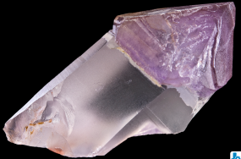
\includegraphics[width=0.5\textwidth]{assets/course/mineral.png}
  \caption{自发形成规则多面体外形的矿物晶体\cite{shi2026xray}}
  \label{fig:crystal-form}
\end{figure}

\subsection{晶体的描述}

描述晶体结构的基本要素包括：空间群（对称性）、晶格常数（晶胞形状）、原子类型、原子
坐标、占有率与位移因子（原子内容）。任何晶体结构都可表述为
\[
\text{晶体结构} = \text{点阵} + \text{结构基元}
\]
其中点阵是对晶体三维周期结构的数学抽象，基元是每个阵点所对应的原子（离子、分子）组。

\subsubsection{原胞与晶胞}

\textbf{点阵（lattice）}：将晶体中周期性重复的环境抽象为几何点（阵点），阵点在三维空间
按一定规律排列形成的无限阵列即为点阵。点阵的平移矢量为
\begin{equation}
  \bm{R}=h\bm{a}+k\bm{b}+l\bm{c} \qquad (h,k,l \text{ 为整数})
\end{equation}
式中 $\bm{a}$、$\bm{b}$、$\bm{c}$ 为基矢。晶体学中常用六种格子：初基 P、体心 I、面心 F、
底心 C、侧心 A、侧心 B（另有三方晶系的 R）。

\begin{figure}[H]
  \centering
  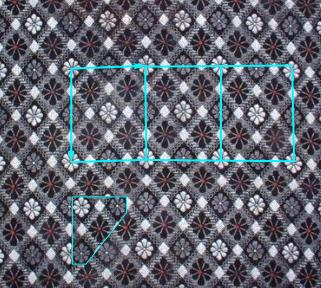
\includegraphics[width=0.4\textwidth]{assets/course/lattice-basis.jpg}
  \caption{点阵示意图：阵点与其平移矢量\cite{shi2026xray}}
  \label{fig:lattice-basis}
\end{figure}

\textbf{初基原胞（primitive cell）}：由三个不共面的基矢所围成的最小平行六面体重复单元。
初基原胞具有体积最小、只含一个格点的特点；但原胞取法不唯一，且往往不能反映晶体的对称性。
在密度泛函（如 VASP）等第一性原理计算中，使用原胞可减小计算量。

\begin{figure}[H]
  \centering
  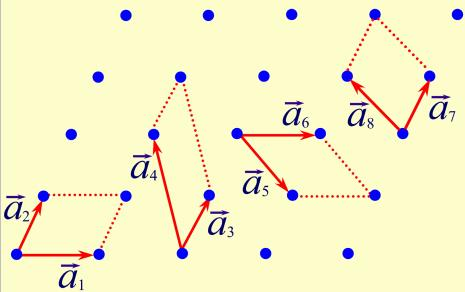
\includegraphics[width=0.5\textwidth]{assets/course/primitive-cell.jpg}
  \caption{由三个基矢构成的初基原胞\cite{shi2026xray}}
  \label{fig:primitive-cell}
\end{figure}

\textbf{晶胞（unit cell，结晶学原胞）}：能够完整反映晶体内部原子（离子）在三维空间分布
的化学--结构特征、并保持晶体对称性且体积尽量小的平行六面体。晶胞的形状由六个晶格参数
（晶格常数）$a$、$b$、$c$、$\alpha$、$\beta$、$\gamma$ 描述，其中 $\alpha=\angle(\bm{b},\bm{c})$、
$\beta=\angle(\bm{a},\bm{c})$、$\gamma=\angle(\bm{a},\bm{b})$。晶胞的选取遵循三条原则：
平行六面体中等棱等角的数目最多、直角最多、体积最小。六个晶格常数的定义见表~\ref{tab:lattice-params}。

\begin{table}[H]
  \centering
  \caption{晶格常数（晶格参数）的定义}
  \label{tab:lattice-params}
  \begin{tabular}{@{}cll@{}}
    \toprule
    符号 & 名称 & 定义 \\
    \midrule
    $a$、$b$、$c$ & 晶轴长度（基矢长度） & 沿三个晶轴方向相邻阵点间的距离 \\
    $\alpha$ & $\bm{b}$ 与 $\bm{c}$ 的夹角 & $\alpha=\angle(\bm{b},\bm{c})$ \\
    $\beta$ & $\bm{a}$ 与 $\bm{c}$ 的夹角 & $\beta=\angle(\bm{a},\bm{c})$ \\
    $\gamma$ & $\bm{a}$ 与 $\bm{b}$ 的夹角 & $\gamma=\angle(\bm{a},\bm{b})$ \\
    \bottomrule
  \end{tabular}
\end{table}

晶胞与原胞之间可通过格点数建立联系。例如体心立方晶胞含 2 个格点，其初基原胞体积为晶胞
体积的 $1/2$，原胞基矢为
\begin{equation}
  \bm{a}_1=\tfrac{1}{2}(-\bm{a}+\bm{b}+\bm{c}),\quad
  \bm{a}_2=\tfrac{1}{2}(\bm{a}-\bm{b}+\bm{c}),\quad
  \bm{a}_3=\tfrac{1}{2}(\bm{a}+\bm{b}-\bm{c})
\end{equation}
面心立方晶胞含 4 个格点，其初基原胞体积为晶胞体积的 $1/4$，原胞基矢为
\begin{equation}
  \bm{a}_1=\tfrac{1}{2}(\bm{a}+\bm{b}),\quad
  \bm{a}_2=\tfrac{1}{2}(\bm{a}+\bm{c}),\quad
  \bm{a}_3=\tfrac{1}{2}(\bm{b}+\bm{c})
\end{equation}

\begin{figure}[H]
  \centering
  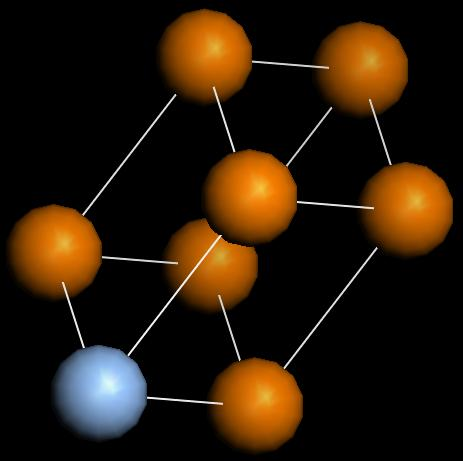
\includegraphics[width=0.4\textwidth]{assets/course/fcc-primitive.jpg}
  \caption{面心立方晶胞与初基原胞的结构模型\cite{shi2026xray}}
  \label{fig:fcc-primitive}
\end{figure}

图~\ref{fig:bcc-cell} 给出了体心立方晶胞与其初基原胞的关系：晶胞顶点与体心处各有一个
原子，虚线所示的初基原胞以晶胞顶点为顶点、以三个相邻晶胞的体心为其余顶点，只含一个格点。

\begin{figure}[H]
  \centering
  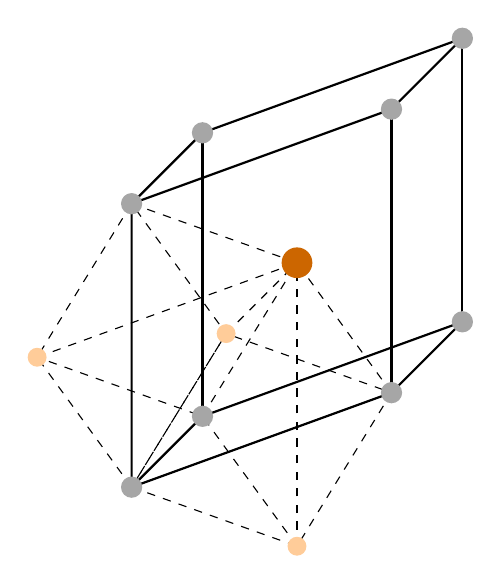
\begin{tikzpicture}[scale=1.5, line join=round]
    % 晶胞顶点（斜投影）：a=(2.2,0.8), b=(0.6,0.6), c=(0,2.4)
    \coordinate (O)   at (0,0);
    \coordinate (A)   at (2.2,0.8);
    \coordinate (B)   at (0.6,0.6);
    \coordinate (C)   at (0,2.4);
    \coordinate (AB)  at (2.8,1.4);
    \coordinate (AC)  at (2.2,3.2);
    \coordinate (BC)  at (0.6,3.0);
    \coordinate (ABC) at (2.8,3.8);
    % 体心
    \coordinate (cen) at (1.4,1.9);
    % 相邻晶胞体心（原胞其余顶点）
    \coordinate (P1) at (-0.8,1.1);  % 1/2(-a+b+c)
    \coordinate (P2) at (0.8,1.3);   % 1/2(a-b+c)
    \coordinate (P3) at (1.4,-0.5);  % 1/2(a+b-c)
    % 晶胞棱（实线）
    \draw[thick] (O)--(A)--(AB)--(B)--cycle;
    \draw[thick] (O)--(C)--(AC)--(ABC)--(BC)--(C);
    \draw[thick] (A)--(AC);
    \draw[thick] (B)--(BC);
    \draw[thick] (AB)--(ABC);
    % 原胞棱（虚线）
    \draw[dashed] (O)--(P1)--(C)--(P2)--cycle;
    \draw[dashed] (O)--(P3)--(A)--(P2);
    \draw[dashed] (O)--(P2);
    \draw[dashed] (P3)--(B)--(P1);
    \draw[dashed] (P3)--(cen);
    \draw[dashed] (P1)--(cen);
    \draw[dashed] (P2)--(cen);
    \draw[dashed] (A)--(cen);
    \draw[dashed] (B)--(cen);
    \draw[dashed] (C)--(cen);
    % 晶胞顶点原子
    \foreach \p in {O,A,B,C,AB,AC,BC,ABC} \fill[gray!70] (\p) circle (0.09);
    % 体心原子（较大）
    \fill[orange!80!black] (cen) circle (0.13);
    % 相邻晶胞体心（较小）
    \foreach \p in {P1,P2,P3} \fill[orange!40] (\p) circle (0.08);
  \end{tikzpicture}
  \caption{体心立方晶胞与初基原胞示意图。实线为晶胞，灰色球为晶胞顶点原子，深色球为
    体心原子；虚线平行六面体为初基原胞，其一个顶点在晶胞顶点处，其余三个顶点为相邻
    晶胞的体心原子（浅色球）。}
  \label{fig:bcc-cell}
\end{figure}

\subsubsection{对称性与空间群}

\textbf{宏观对称元素}指晶体的宏观性质所反映的对称性，包括四类独立对称元素：

\begin{itemize}
  \item \textbf{旋转轴 $n$}：晶体绕某一几何直线旋转 $2\pi/n$ 后复原。由于晶体周期性的
    限制，旋转轴只可能是 1、2、3、4、6 次轴。设沿周期方向相邻两阵点 A、B，绕 A 点轴
    旋转 $\theta$ 角后 B 移到 B$'$，B$'$ 仍必须是阵点，故
    $A'B'=AB-2AB\cos\theta=n\,AB$（$n$ 为整数），解得
    $\cos\theta = 0,\,\tfrac12,\,1$，对应 $\theta=90^\circ,60^\circ,0^\circ$（另一半解
    同理），即只存在 2、3、4、6 次轴。准晶（如 1984 年发现的五重对称准晶）因失去长程
    平移周期性而允许 5 次轴。
  \item \textbf{镜面 $m$}：晶体经某一平面反映后复原，操作前后两原子位于镜面同一法向的
    两侧且等距反向。
  \item \textbf{反演中心 $\bar{1}$}：晶体经某一点反演后复原，操作前后两原子位于同一直线
    上、等距反向。
  \item \textbf{旋转反演轴 $\bar{n}$}：旋转 $2\pi/n$ 与反演的联合操作。例如
    $\bar{3}=3+\bar{1}$，$\bar{6}=3/m$（三重旋转加镜面）。
\end{itemize}

\begin{figure}[H]
  \centering
  \subcaptionbox{旋转、反演与镜面操作示意}{%
    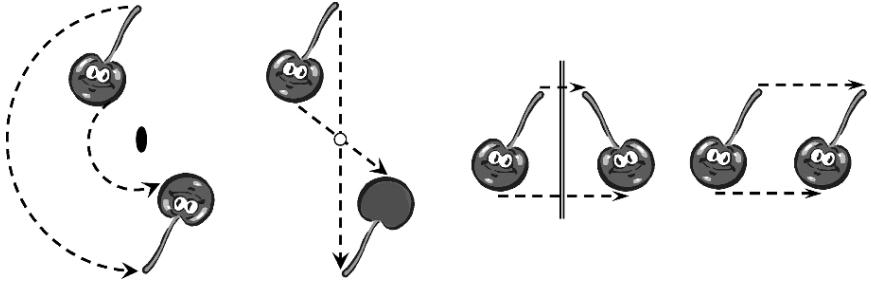
\includegraphics[width=0.62\textwidth]{assets/course/macro-sym.jpg}}

  \subcaptionbox{旋转轴次数的周期性证明示意}{%
    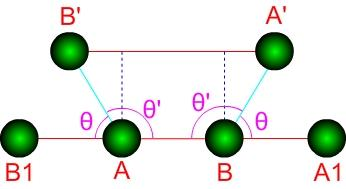
\includegraphics[width=0.55\textwidth]{assets/course/fivefold-proof.jpg}}
  \caption{宏观对称元素与晶体中旋转轴次数的限制\cite{shi2026xray}}
  \label{fig:macro-sym}
\end{figure}

\begin{figure}[H]
  \centering
  \subcaptionbox{P1 与 P$\bar1$ 中反演中心的作用}{%
    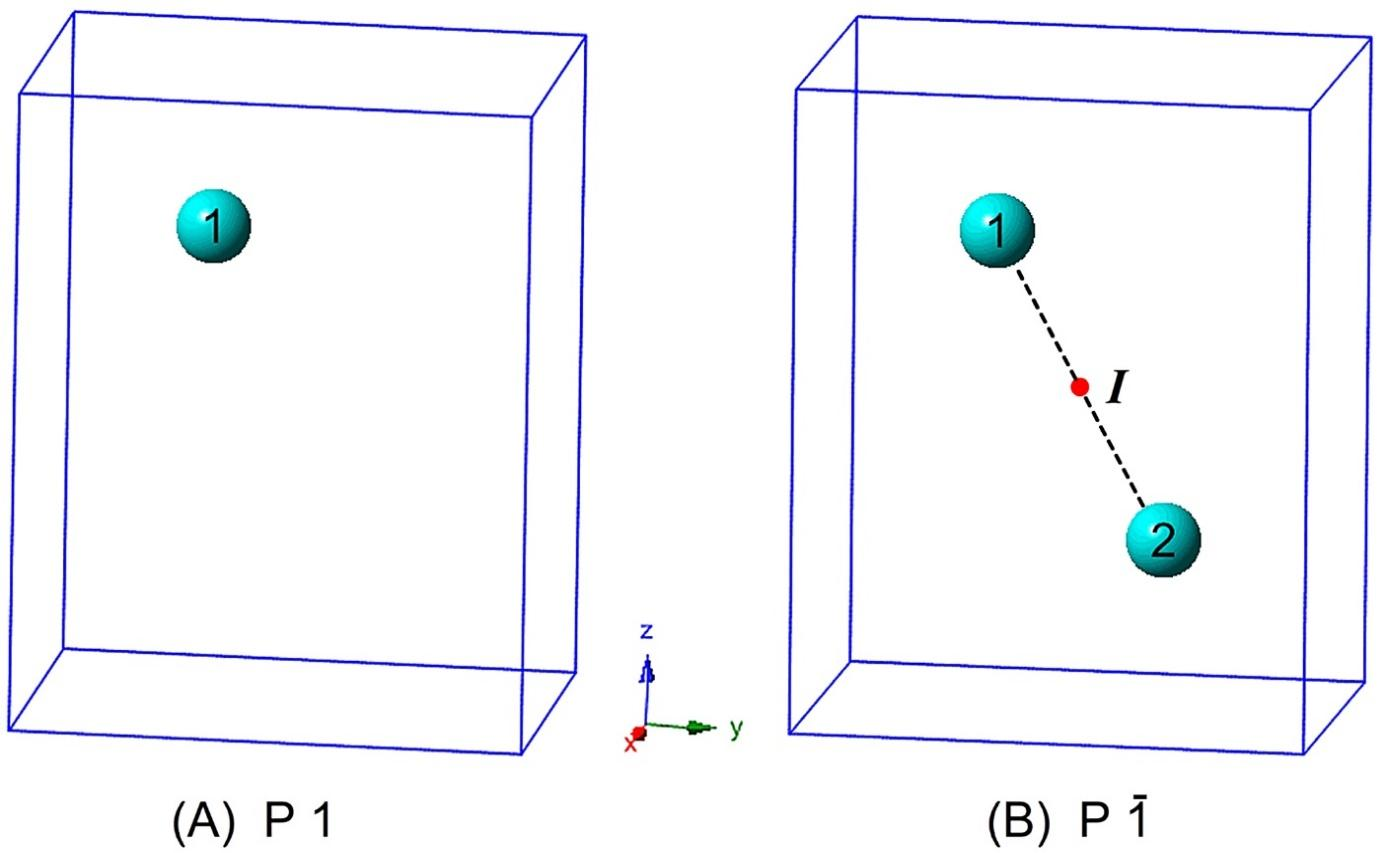
\includegraphics[width=0.52\textwidth]{assets/course/inversion.jpg}}

  \subcaptionbox{P3、P$\bar3$、P6、P$\bar6$ 中的旋转轴与旋转反演轴}{%
    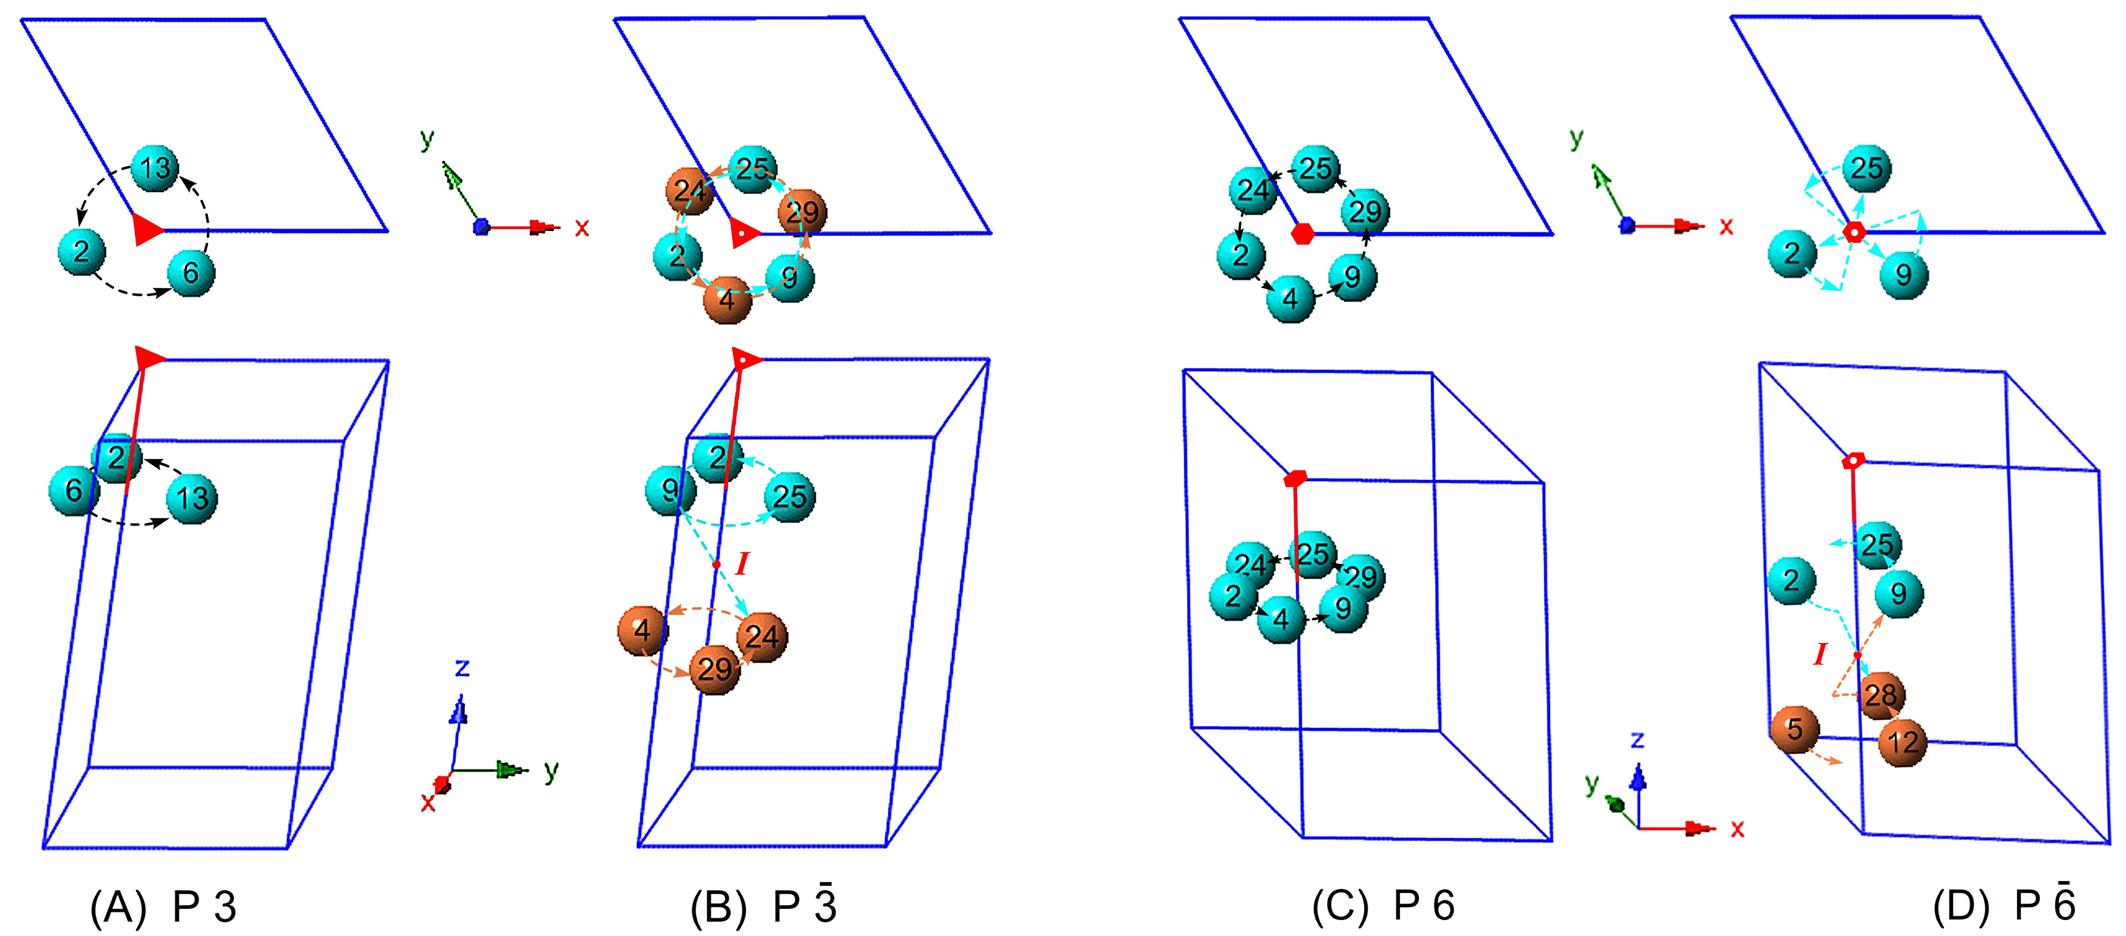
\includegraphics[width=0.5\textwidth]{assets/course/rotation-axis.jpg}}
  \hfill
  \subcaptionbox{P$m$ 中的镜面操作}{%
    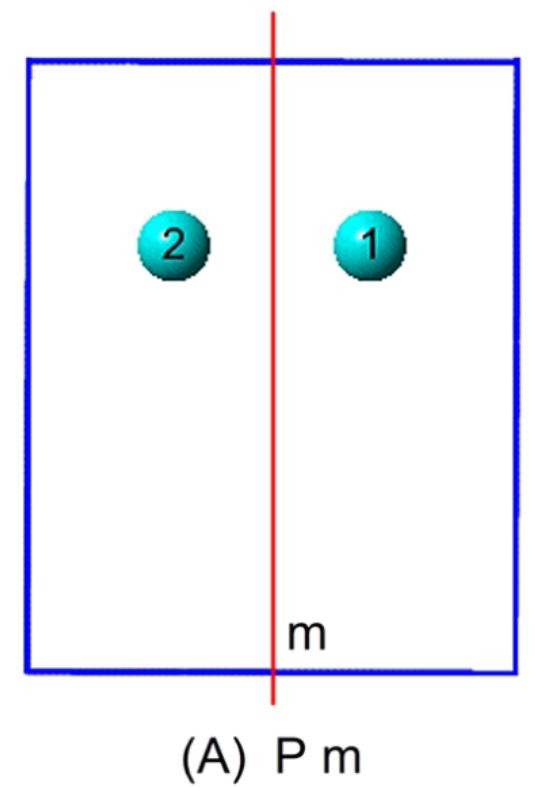
\includegraphics[width=0.24\textwidth]{assets/course/mirror.jpg}}
  \caption{利用 Diamond 观察宏观对称元素\cite{shi2026xray}}
  \label{fig:sym-diamond}
\end{figure}

宏观对称元素的组合共形成 \textbf{32 种点群}；按点群对称特征，晶体划分为 7 大晶系，
对应 14 种 Bravais 格子（表~\ref{tab:crystalsystems}）。在无限晶体中，平移本身也是
对称操作，并且还允许包含平移的\textbf{微观对称元素}——\textbf{螺旋轴}与\textbf{滑移
面}。螺旋轴 $n_m$ 是旋转 $2\pi/n$ 与沿轴方向平移 $m/n$ 个晶格周期单位的联合操作：经
$n$ 次操作后原子到达等效位置，而中间位置均不在同一平面上，沿轴呈螺旋状排列
（图~\ref{fig:micro-sym}(a)(b)）；滑移面是镜面反映与沿面内特定方向平移的联合操作，
包括沿 $a$、$b$、$c$ 方向平移 $1/2$ 的轴滑移面、沿面对角线方向平移 $1/2$ 的对角滑移面
$n$，以及平移 $1/4$ 的金刚石滑移面 $d$（图~\ref{fig:micro-sym}(c)）。宏观与微观对称
元素相互组合，共形成 \textbf{230 种空间群}\cite{hahn2005itt}。

\begin{figure}[H]
  \centering
  \subcaptionbox{$6_1$ 螺旋轴的操作路径（旋转 $60^\circ$ 加平移 $1/6$）}{%
    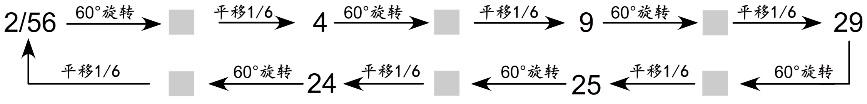
\includegraphics[width=0.82\textwidth]{assets/course/screw61.jpg}}

  \subcaptionbox{$6_5$ 螺旋轴的操作路径（旋转 $300^\circ$ 加平移 $1/6$）}{%
    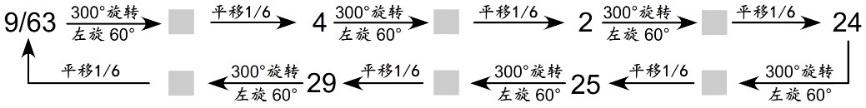
\includegraphics[width=0.82\textwidth]{assets/course/screw65.jpg}}

  \subcaptionbox{$c$ 滑移面的操作（镜面加平移 $1/2$）}{%
    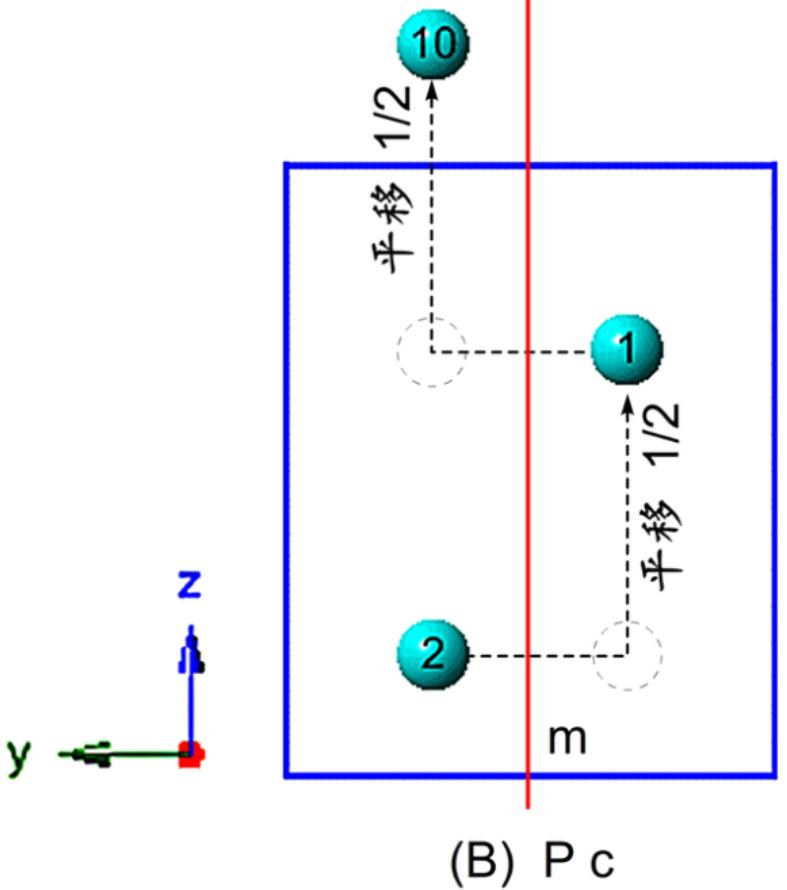
\includegraphics[width=0.3\textwidth]{assets/course/glide.jpg}}
  \caption{微观对称元素——螺旋轴与滑移面\cite{shi2026xray}}
  \label{fig:micro-sym}
\end{figure}

\begin{table}[H]
  \centering
  \small
  \caption{七大晶系、特征对称元素与 Bravais 格子}
  \label{tab:crystalsystems}
  \begin{tabular}{@{}llll@{}}
    \toprule
    晶系 & 晶格参数特征 & 特征对称元素 & Bravais 格子 \\
    \midrule
    三斜 & $a\ne b\ne c$，$\alpha\ne\beta\ne\gamma$ & 1 或 $\bar1$ & P \\
    单斜 & $a\ne b\ne c$，$\alpha=\gamma=90^\circ\ne\beta$ & 一个 2 次轴或镜面 & P, C \\
    正交 & $a\ne b\ne c$，$\alpha=\beta=\gamma=90^\circ$ & 三个互相垂直的 2 次轴（或镜面） & P, C, I, F \\
    四方 & $a=b\ne c$，$\alpha=\beta=\gamma=90^\circ$ & 一个 4 次轴 & P, I \\
    三方 & $a=b=c$，$\alpha=\beta=\gamma\ne90^\circ$ & 一个 3 次轴 & R \\
    六方 & $a=b\ne c$，$\alpha=\beta=90^\circ$，$\gamma=120^\circ$ & 一个 6 次轴 & P \\
    立方 & $a=b=c$，$\alpha=\beta=\gamma=90^\circ$ & 四个 3 次轴（沿体对角线） & P, I, F \\
    \bottomrule
  \end{tabular}
\end{table}

\begin{figure}[H]
  \centering
  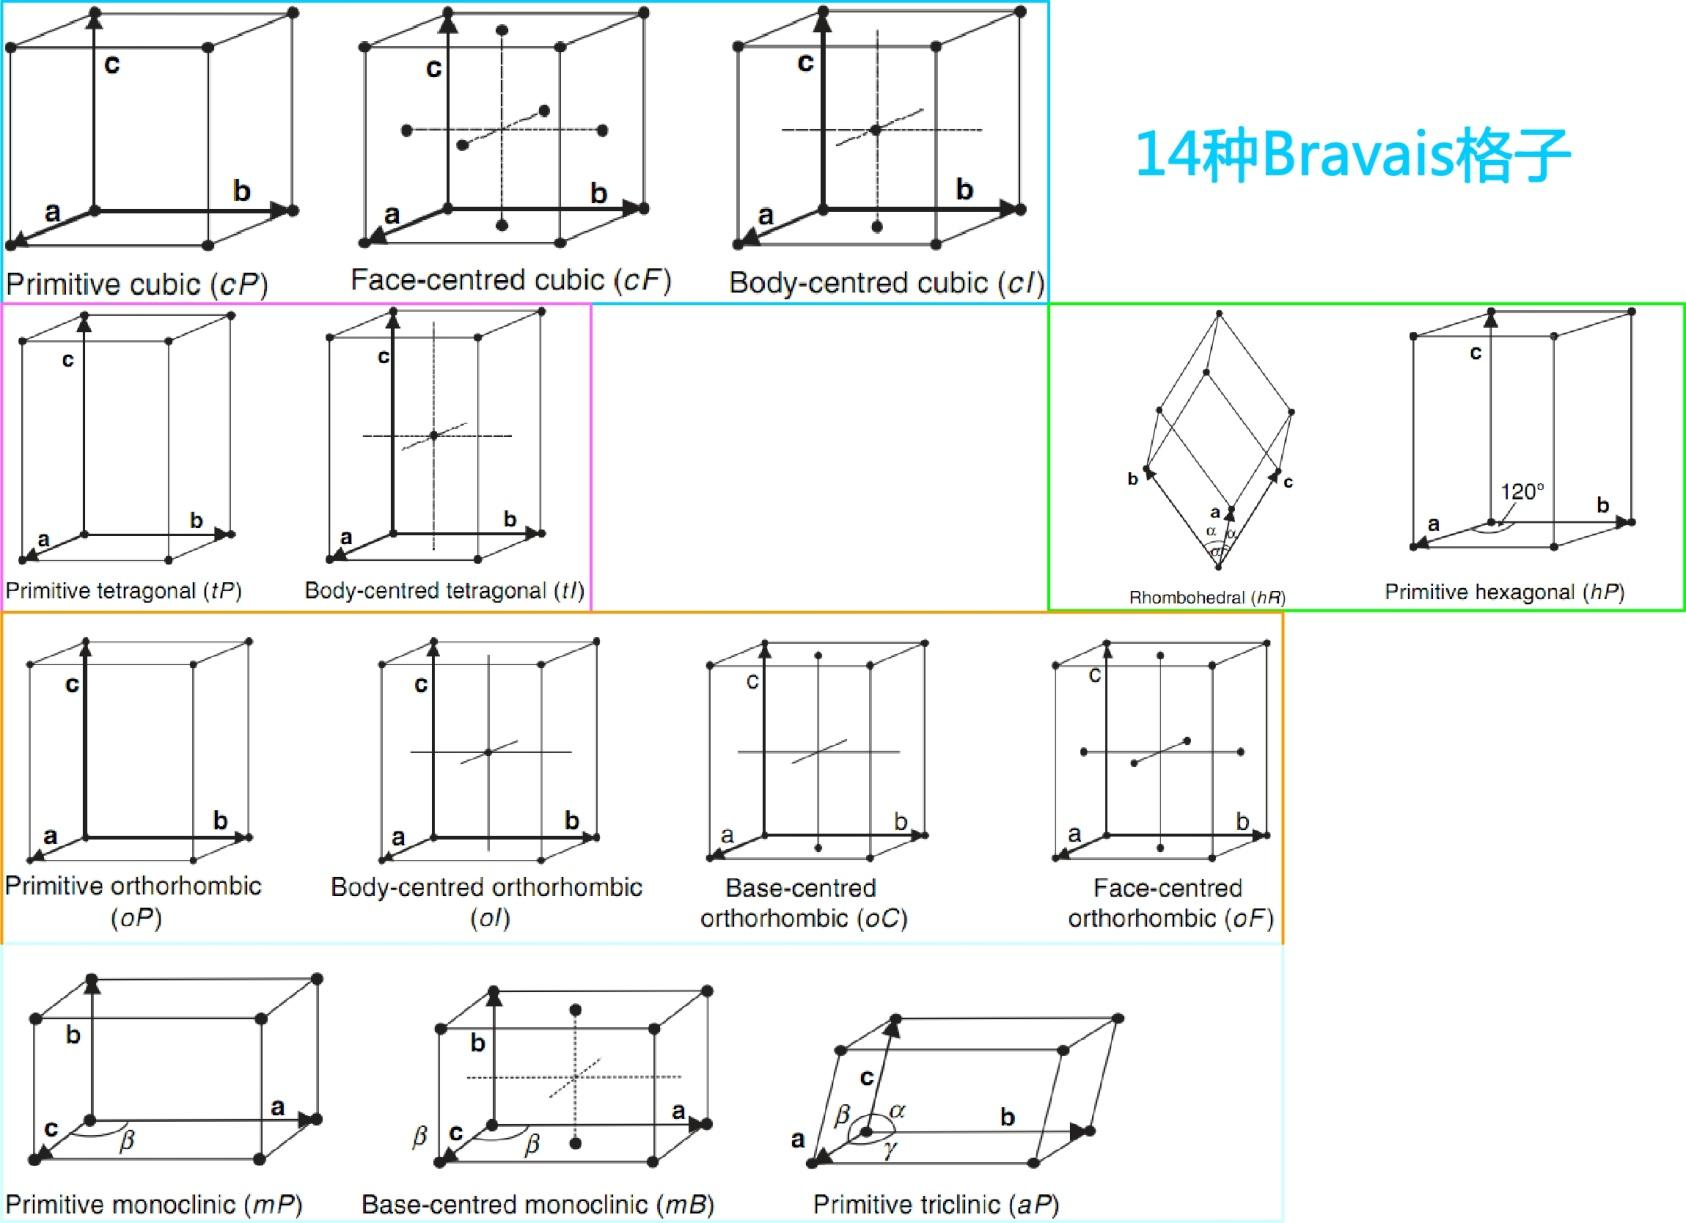
\includegraphics[width=0.75\textwidth]{assets/course/bravais-types.jpg}
  \caption{14 种 Bravais 格子\cite{shi2026xray}}
  \label{fig:bravais14}
\end{figure}

空间群的\textbf{国际符号}由点阵类型字母（P、F、I、A、B、C、R）与三个特征方向（由晶系
决定，见表~\ref{tab:crystalsystems}）上的对称元素符号组成。例如立方晶系的三个特征方向
依次为 [100]、[111]、[110]。据此：
$F\,m\,\bar3\,m$ 表示面心立方点阵，[100] 方向为镜面 $m$，[111] 方向为旋转反演轴
$\bar3$（立方晶系的特征），[110] 方向为镜面 $m$；$P\,6_3/m\,m\,c$ 表示六方初基点阵，
[001] 方向为 $6_3$ 螺旋轴加镜面，[100] 方向为镜面，[120] 方向为 $c$ 滑移面；
$P\,4_2/m\,n\,m$ 表示四方初基点阵，[001] 方向为 $4_2$ 螺旋轴加镜面；$I\,4_1/a\,m\,d$
表示体心四方点阵，[001] 方向为 $4_1$ 螺旋轴加 $a$ 滑移面，[100] 方向为镜面，[110]
方向为 $d$ 金刚石滑移面。

\begin{figure}[H]
  \centering
  \subcaptionbox{三斜至四方晶系}{%
    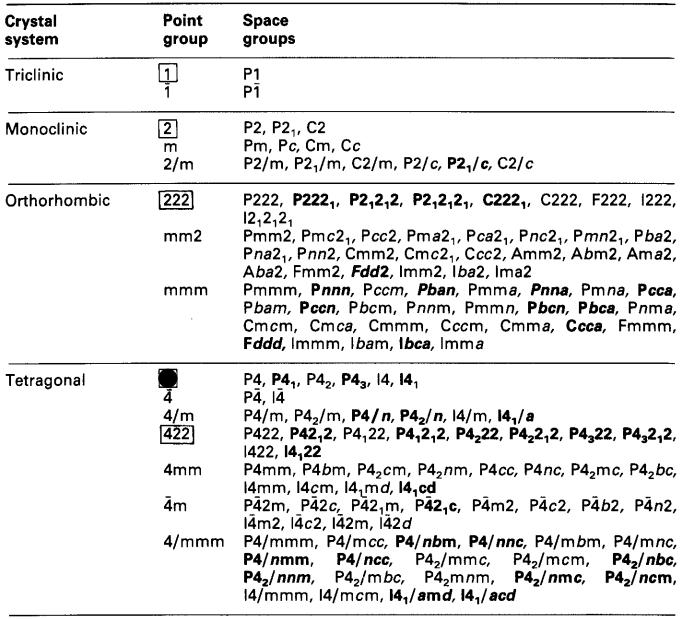
\includegraphics[width=0.42\textwidth]{assets/course/spacegroup-symbol.jpg}}
  \hfill
  \subcaptionbox{三方（六方）与立方晶系}{%
    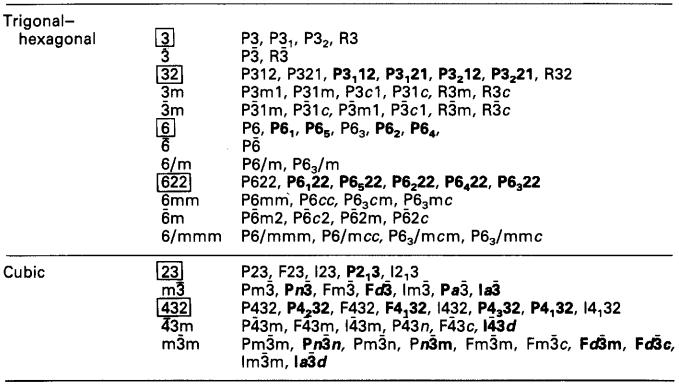
\includegraphics[width=0.42\textwidth]{assets/course/spacegroup-projection.jpg}}
  \caption{七大晶系中空间群与点群的对应关系\cite{shi2026xray}}
  \label{fig:spacegroup-table}
\end{figure}

\subsubsection{晶胞内的原子}

确定空间群与晶格常数后，还需给出晶胞内原子的\textbf{种类}、\textbf{分数坐标} $(x,y,z)$、
\textbf{占有率}（占位度）与\textbf{位移因子}（描述原子在平衡位置附近的热振动）等参数。
由于空间群对称操作的作用，只需给出非对称单元（asymmetric unit）中不等价原子的参数，
即可生成晶胞内全部等价原子。空间群表中以 \textbf{Wyckoff 位}给出各类可能占位：多重度
（multiplicity）表示在该位放一个原子时晶胞内出现几个等效原子，位点对称性（site
symmetry）表示该位所保持的对称性；多重度等于一般位置的多重度的位置称一般位，否则为
特殊位。表~\ref{tab:wyckoff} 以 $F\,m\,\bar3\,m$ 空间群为例列出了全部 Wyckoff 位。

\begin{table}[H]
  \centering
  \caption{$F\,m\,\bar3\,m$ 空间群的 Wyckoff 位（多重度、位点对称性与坐标）}
  \label{tab:wyckoff}
  \begin{tabular}{@{}cclc@{}}
    \toprule
    序号 & 坐标 & 多重度 & 位点对称性 \\
    \midrule
    1  & $(x,y,z)$           & 192 & $1$ \\
    2  & $(x,x,z)$           & 96  & $..m$ \\
    3  & $(x,y,0)$           & 96  & $m..$ \\
    4  & $(x,x,1/2)$         & 48  & $m.m2$ \\
    5  & $(x,x,0)$           & 48  & $m.m2$ \\
    6  & $(x,x+1/4,1/4)$     & 48  & $2.mm$ \\
    7  & $(x,x,x)$           & 32  & $.3m$ \\
    8  & $(x,0,0)$           & 24  & $4m.m$ \\
    9  & $(0,1/4,1/4)$       & 24  & $.m.mm$ \\
    10 & $(1/4,1/4,1/4)$     & 8   & $\bar43m$ \\
    11 & $(0,0,1/2)$         & 4   & $m\bar3m$ \\
    12 & $(0,0,0)$           & 4   & $m\bar3m$ \\
    \bottomrule
  \end{tabular}
\end{table}

晶胞中的化学式单元数 $Z$ 可由实测密度与晶胞体积确定：
\begin{equation}
  Z=\frac{\rho V N_A}{M}
\end{equation}
其中 $\rho$ 为密度（g/cm$^3$）、$V$ 为晶胞体积（cm$^3$）、$N_A$ 为阿伏伽德罗常数、
$M$ 为摩尔质量。$Z$ 是检验指标化与结构解析结果是否合理的重要判据。将上述结构信息
（空间群、晶格参数与原子参数）按统一格式存储，即得到晶体学信息文件（CIF 文件），
它可被 Diamond 等软件直接读取用于建模。

\begin{figure}[H]
  \centering
  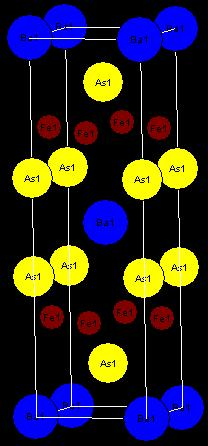
\includegraphics[width=0.28\textwidth]{assets/course/structure-elements.jpg}
  \caption{晶体结构模型示例：描述晶体结构所需的全部要素（空间群、晶格常数与原子参数）
    \cite{shi2026xray}}
  \label{fig:structure-elements}
\end{figure}

% ==================== 2.3 晶体的可视化 ====================
\subsection{晶体的可视化}

晶体结构是三维的，平面文字与二维投影图难以直观表达原子在空间中的排布、对称关系与配位
环境。晶体结构可视化软件（如 Diamond、VESTA、CrystalMaker 等）可将空间群、晶格常数与
原子坐标转化为可旋转、可缩放的三维模型，并支持晶面、配位多面体与粉末衍射谱的显示，
是学习晶体学的有力工具。下面以 Diamond 软件为例，介绍晶体结构的建模过程，并对八种常见
晶体结构逐一建模、图文讲解其结构特征\cite{diamond2023manual}。

\subsubsection{利用 Diamond 软件建立晶体结构模型}

本节以体心立方铁（空间群 $I\,m\,\bar3\,m$，$a=2.819$\,\AA）为例，说明从零开始建立
晶体结构模型的完整操作流程。

\textbf{（1）新建文档。}执行 File $\to$ New 命令，在弹出的 ``New Document'' 对话框中
选择 ``Create a document and type in or modify structure parameters''（创建一个文档并
输入或修改结构参数），如图~\ref{fig:dia-newdoc} 所示。

\begin{figure}[H]
  \centering
  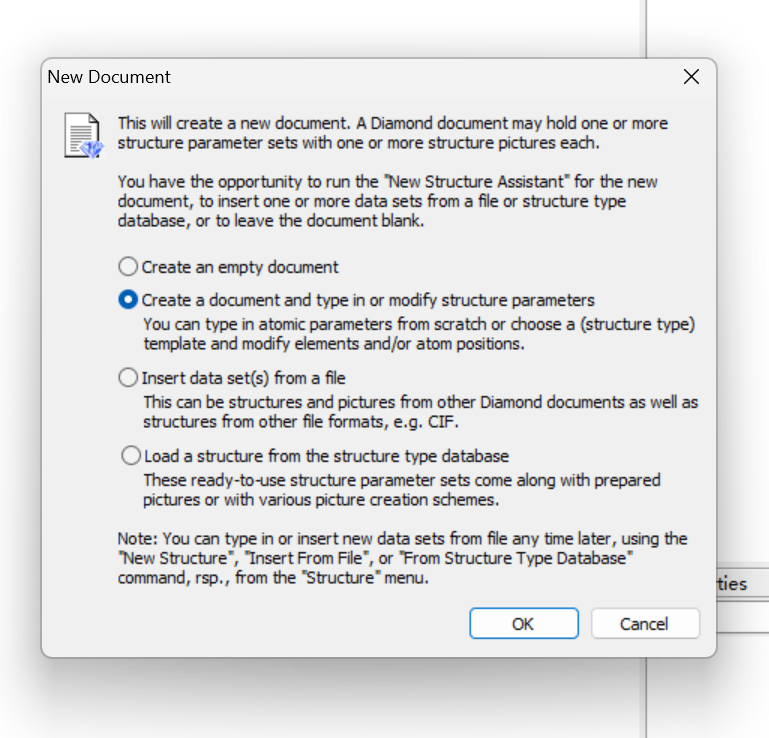
\includegraphics[width=0.52\textwidth]{assets/workflow/01-new-document.png}
  \caption{Diamond 软件的 New Document 对话框}
  \label{fig:dia-newdoc}
\end{figure}

\textbf{（2）选择晶体数据来源。}进入 ``New Structure'' 向导后，在 ``Source of structure
data'' 页选择 ``Type in new structure parameters''（输入新的结构参数），
如图~\ref{fig:dia-source} 所示。

\begin{figure}[H]
  \centering
  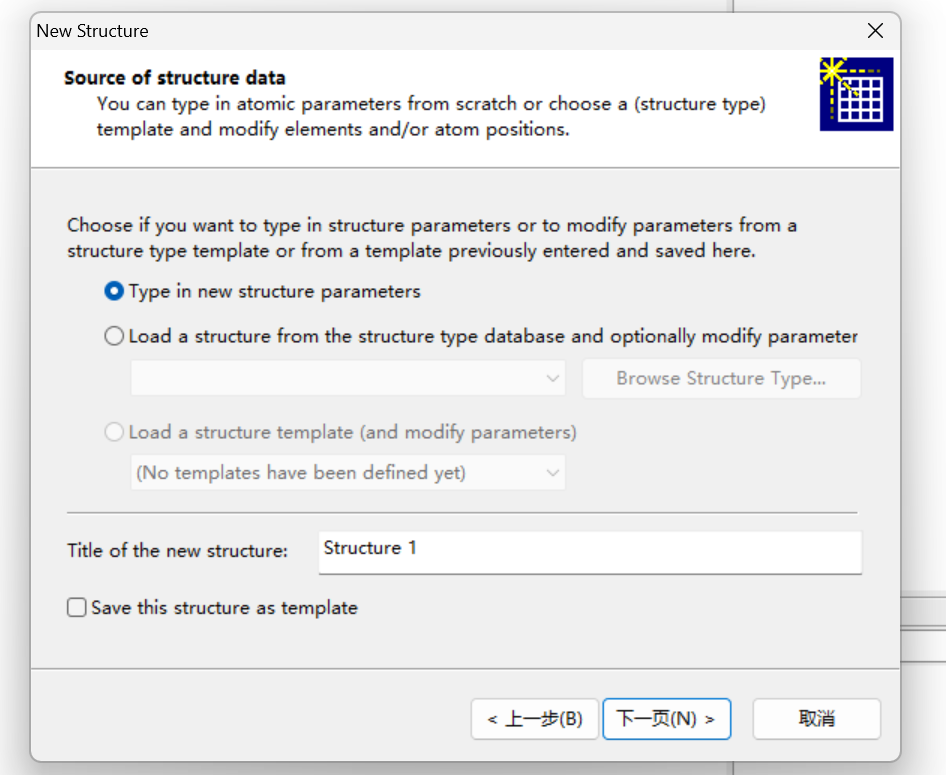
\includegraphics[width=0.52\textwidth]{assets/workflow/02-data-source.png}
  \caption{选择结构数据来源：直接输入新的结构参数}
  \label{fig:dia-source}
\end{figure}

\textbf{（3）设置空间群与晶格常数。}在 ``Cell parameters and space group'' 页通过
Browse 选择空间群（此处为 $I\,m\,\bar3\,m$ (229)），并输入晶格常数 $a$、$b$、$c$ 与
$\alpha$、$\beta$、$\gamma$（此处 $a=b=c=2.819$\,\AA，$\alpha=\beta=\gamma=90^\circ$），
如图~\ref{fig:dia-cell}(a) 所示。\textbf{注意事项}：空间群必须与晶系及晶格常数的关系
自洽，例如立方晶系要求 $a=b=c$ 且 $\alpha=\beta=\gamma=90^\circ$；若输入有误，可通过
Structure $\to$ Symmetry 修改空间群，再用 Build $\to$ Fill $\to$ Unit Cell 重建。

\textbf{（4）添加原子。}在 ``Atomic parameters'' 页输入元素种类与分数坐标 $x$、$y$、
$z$，点击 Add 将原子加入非对称单元，如图~\ref{fig:dia-cell}(b) 所示。通常只需输入
非对称单元中的不等价原子，Diamond 将依据空间群的对称操作自动生成晶胞内全部等价原子。

\begin{figure}[H]
  \centering
  \subcaptionbox{空间群与晶格常数设置\label{fig:dia-cell-a}}{%
    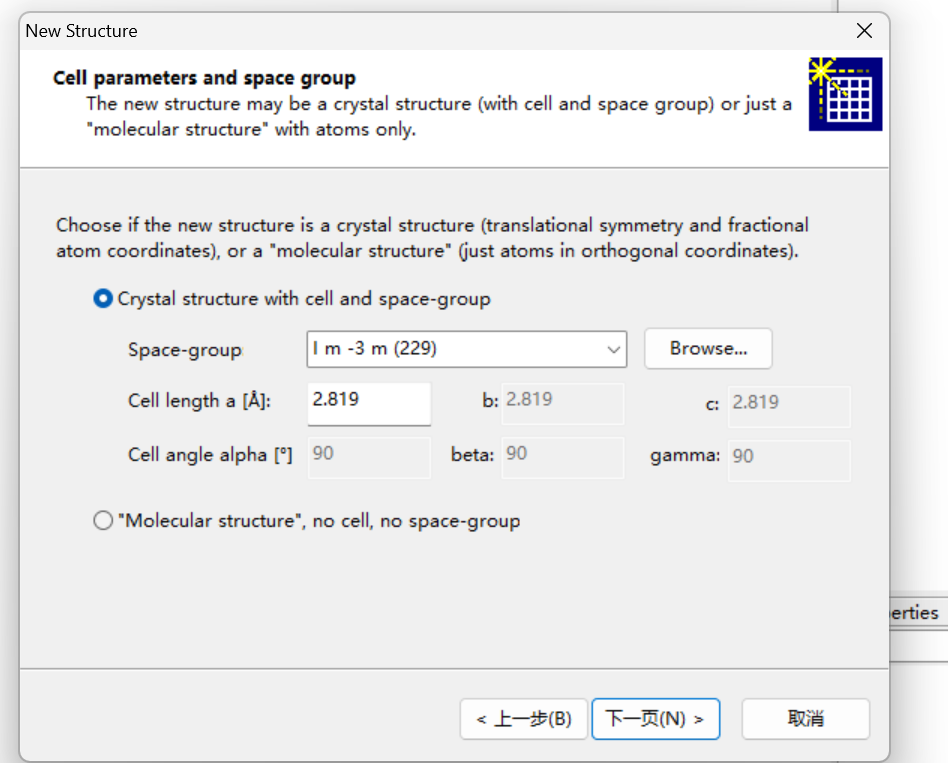
\includegraphics[width=0.44\textwidth]{assets/workflow/03-cell-parameters.png}}
  \hfill
  \subcaptionbox{原子参数（分数坐标）添加\label{fig:dia-cell-b}}{%
    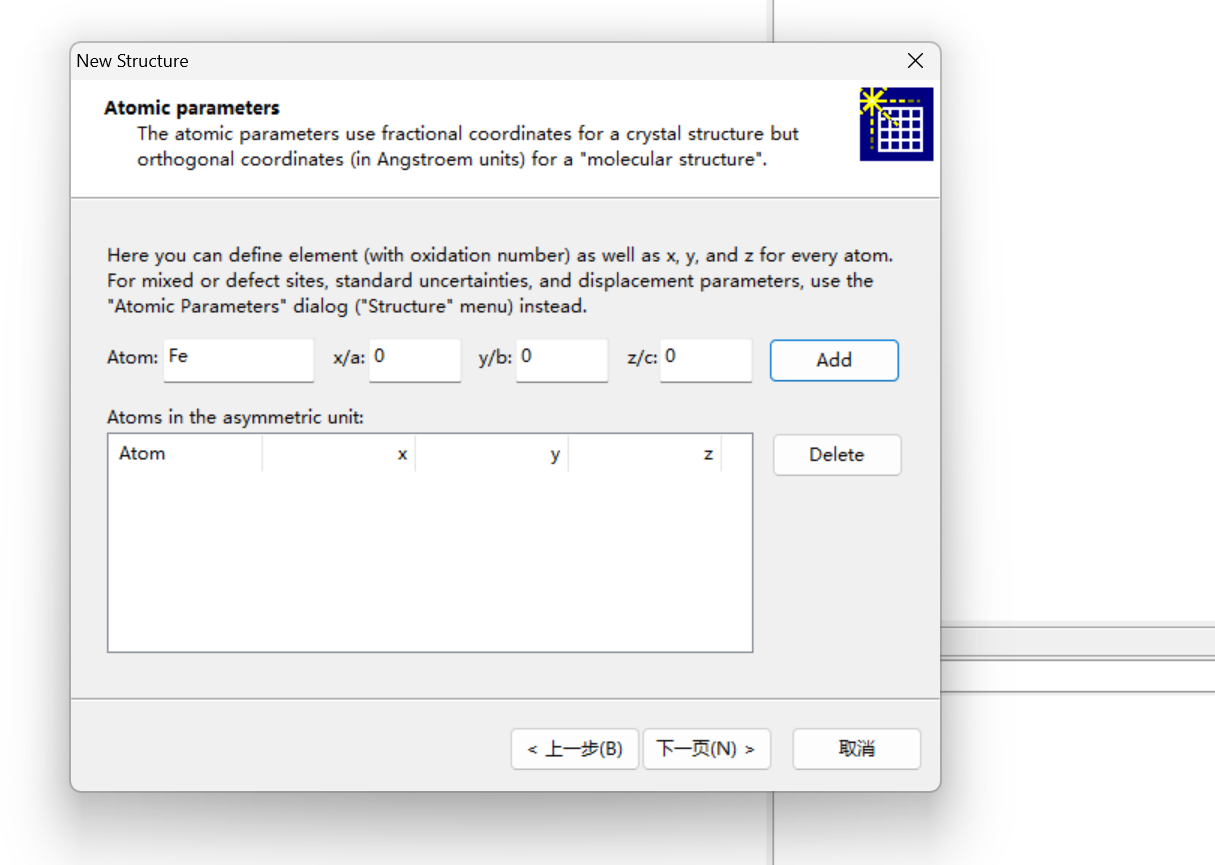
\includegraphics[width=0.46\textwidth]{assets/workflow/04-add-atoms.png}}
  \caption{Diamond 建模向导中的晶胞参数设置与原子添加}
  \label{fig:dia-cell}
\end{figure}

\textbf{（5）填充晶胞与扩展显示。}执行 Build $\to$ Fill $\to$ Unit Cell 生成一个晶胞的
结构模型；执行 Build $\to$ Fill $\to$ Box（或 Range）可显示多个相邻晶胞，以便观察结构
的周期延伸；若需恢复单胞显示，删除全部原子后用 Unit Cell 重建即可。

\textbf{（6）视图与外观设置。}按住鼠标拖动可实时旋转、缩放模型，选择合适的观察方向；
右键原子执行 Edit $\to$ Atom Design 可设置原子颜色与显示半径；选中原子后右键执行
Add $\to$ Atom Labels，可将标签类型设为 Atom Identifier、格式设为 ATOM \#，给原子编号，
便于追踪对称操作前后原子的对应关系。

\textbf{（7）建立晶面。}执行 Objects $\to$ Planes $\to$ Create Lattice Plane，输入
Miller 指数 $(h\,k\,l)$ 与位置（以 $d$ 间距的倍数表示），即可在模型中添加晶面，
如图~\ref{fig:dia-plane} 所示（图中为 BCC 铁的 (111) 晶面，$d=1.6276$\,\AA）。在右侧
Tables of Planes 面板中右键某晶面可进入 Shift Plane Mode，沿晶面法线方向拖动晶面；
执行 Build $\to$ Fill $\to$ Slab 则可显示晶面及其上下指定范围内的原子，便于观察密排面。

\begin{figure}[H]
  \centering
  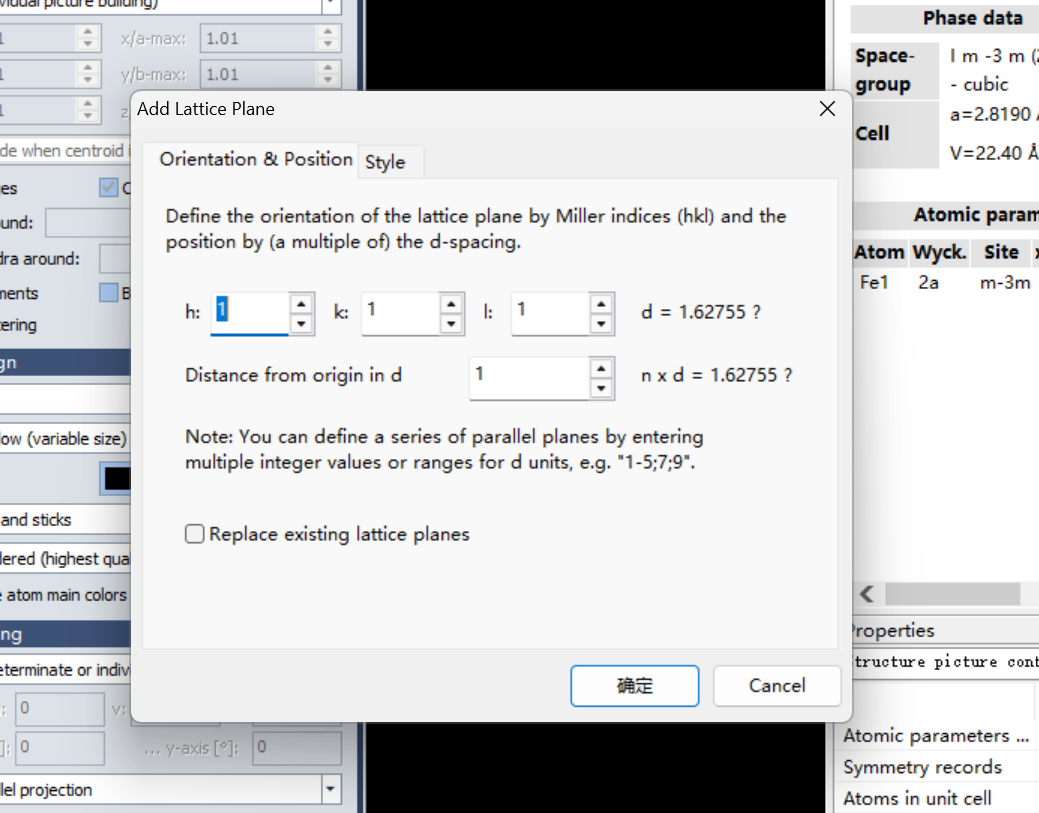
\includegraphics[width=0.52\textwidth]{assets/workflow/08-add-lattice-plane.png}
  \caption{Add Lattice Plane 对话框：输入 Miller 指数与晶面位置}
  \label{fig:dia-plane}
\end{figure}

\textbf{（8）添加配位多面体。}执行 Build $\to$ Polyhedra $\to$ Add Coordination
Polyhedra，在对话框中选择中心原子与配位原子并设置键长范围，即可显示配位多面体，
如图~\ref{fig:dia-poly} 所示。若只想观察特定原子的配位环境，可先选中该原子作为中心再
调用此功能。通过观察配位多面体之间共角、共棱、共面的连接方式，可以理解配位体如何
堆积、键合进而形成晶体（三种连接方式的稳定性依次降低）。

\begin{figure}[H]
  \centering
  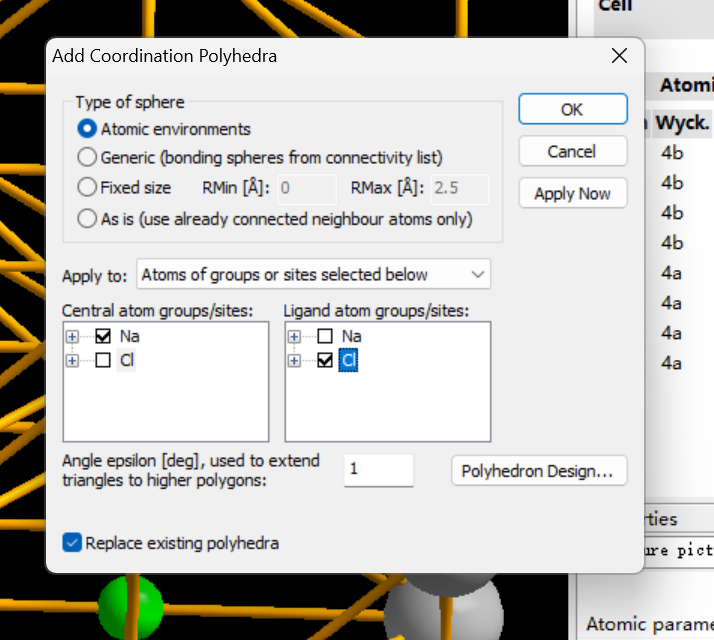
\includegraphics[width=0.46\textwidth]{assets/workflow/09-add-coordination-polyhedra.png}
  \caption{Add Coordination Polyhedra 对话框：选择中心原子与配位原子}
  \label{fig:dia-poly}
\end{figure}

\textbf{（9）模拟 X 射线粉末衍射图。}执行 View $\to$ Powder Pattern
（图~\ref{fig:dia-xrd}(a)），在衍射设置中选择 X 射线模式、波长与 $2\theta$ 范围等参数
（图~\ref{fig:dia-xrd}(b)(c)），即可得到该晶体结构的理论粉末衍射谱，用于与实际 XRD
图谱对比。

\begin{figure}[H]
  \centering
  \subcaptionbox{View 菜单中的 Powder Pattern 命令}{%
    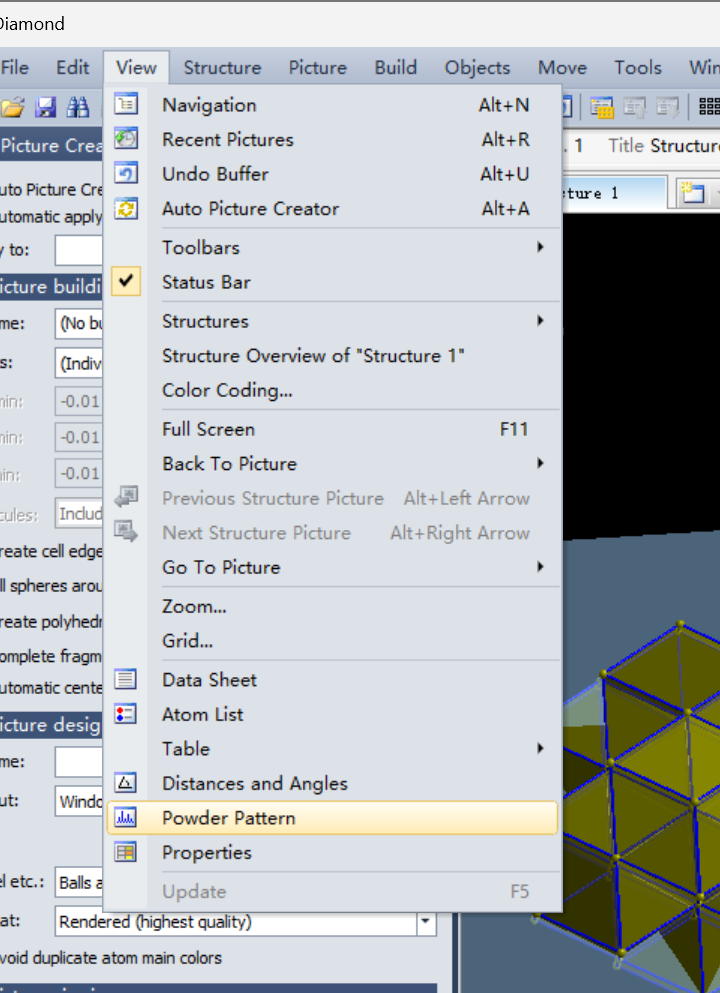
\includegraphics[width=0.30\textwidth]{assets/workflow/05-view-powder-pattern.png}}
  \hfill
  \subcaptionbox{选择 XRD 衍射模式}{%
    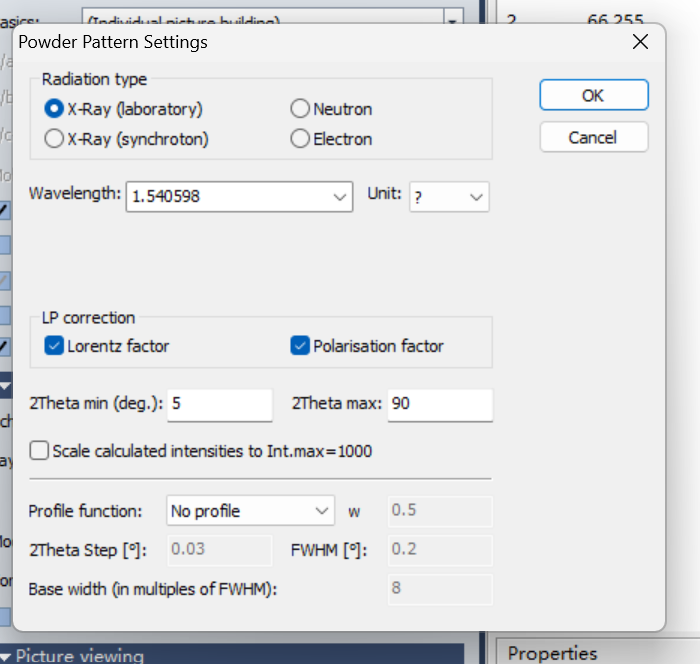
\includegraphics[width=0.30\textwidth]{assets/workflow/06-xrd-mode.png}}
  \hfill
  \subcaptionbox{XRD 模拟参数设置}{%
    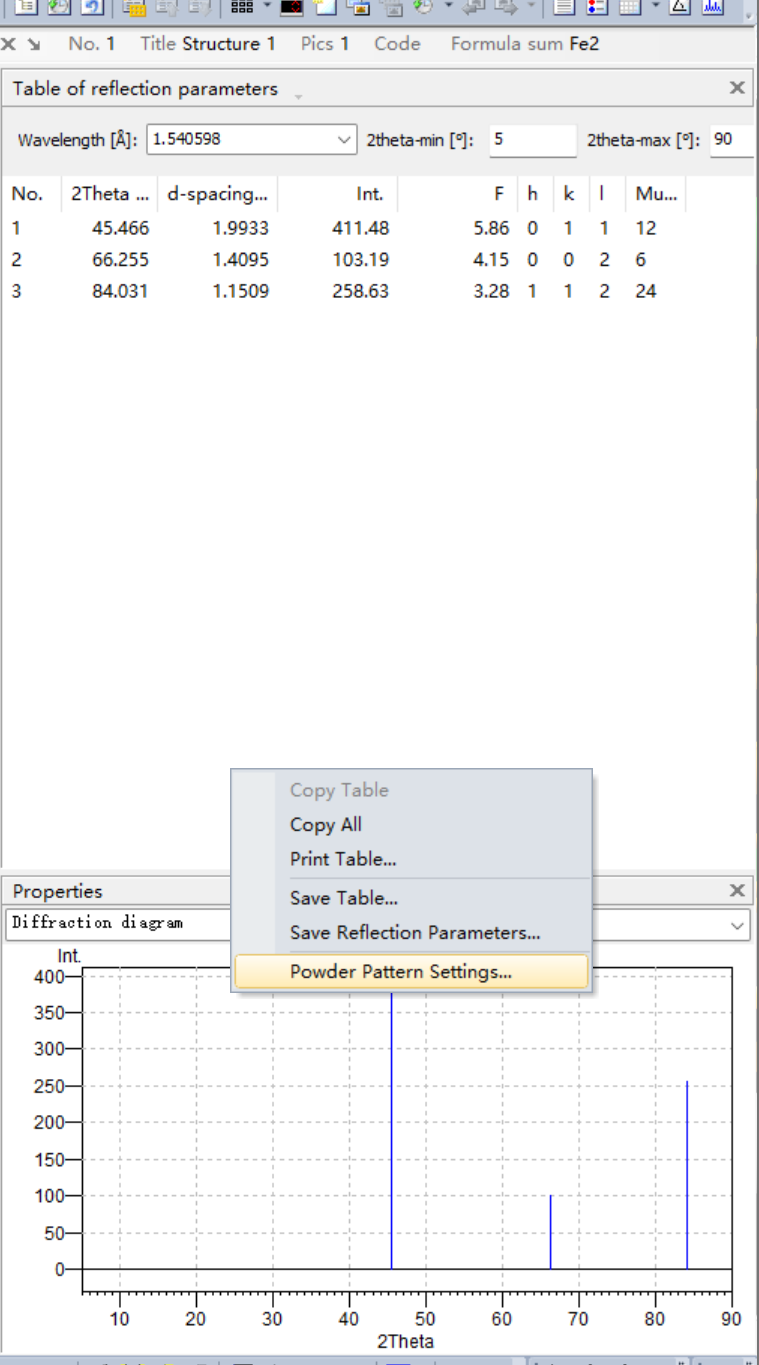
\includegraphics[width=0.30\textwidth]{assets/workflow/07-xrd-settings.png}}
  \caption{Diamond 中粉末衍射图的模拟}
  \label{fig:dia-xrd}
\end{figure}

\textbf{（10）测量工具。}利用 Tools 菜单中的距离与角度测量功能，可测定键长、键角与
晶面间距，用于定量验证结构特征。

归纳起来，Diamond 建模与观察的要点包括：空间群、晶系与晶格常数必须自洽；原子坐标采用
分数坐标，只需输入非等效原子；统计晶胞内原子数时，顶点原子计 $1/8$、棱上原子计 $1/4$、
面上原子计 $1/2$、内部原子计 $1$；在钢球模型下，先找密排方向（密排线），由原子相切
条件求出原子半径，即可计算原子堆积因子（体积占有率）；配位多面体的连接方式（共角、
共棱、共面）反映了配位体堆积的稳定性。

\subsubsection{常见晶体结构的特征}

下面利用上述建模方法，对八种常见晶体结构逐一建立模型并讲解其结构特征。每种结构均给出
建模参数（空间群、晶格常数、非对称单元原子坐标与化学式单元数 $Z$），并结合结构模型图、
理论粉末衍射图、密堆积晶面图与配位多面体图进行分析；文中所有截图均由 Diamond 软件生成。

% ==================== 2.3.2.1 FCC ====================
\jiegou{2.3.2.1}{面心立方结构（FCC）}

面心立方（FCC）是最常见的金属结构之一，本次以铁为对象建模。空间群取 $F\,m\,\bar3\,m$
（立方晶系，No.~225），晶格常数、原子坐标与化学式单元数一并列于表~\ref{tab:fcc}。
非对称单元里只需填 1 个 Fe 原子，晶胞内的其余原子由软件的对称操作自动补出。

\begin{table}[H]
  \centering
  \caption{面心立方（FCC）结构的建模参数}
  \label{tab:fcc}
  \begin{tabular}{ll}
    \toprule
    项目 & 参数 \\
    \midrule
    空间群 & $F\,m\,\bar3\,m$（No.~225） \\
    晶格常数 & $a=b=c=3.43$\,\AA，$\alpha=\beta=\gamma=90^\circ$ \\
    原子坐标 & Fe：$(0,0,0)$（$4a$ 位） \\
    化学式单元数 & $Z=4$ \\
    \bottomrule
  \end{tabular}
\end{table}

\begin{figure}[H]
  \centering
  \subcaptionbox{空间群与晶格常数设置}{%
    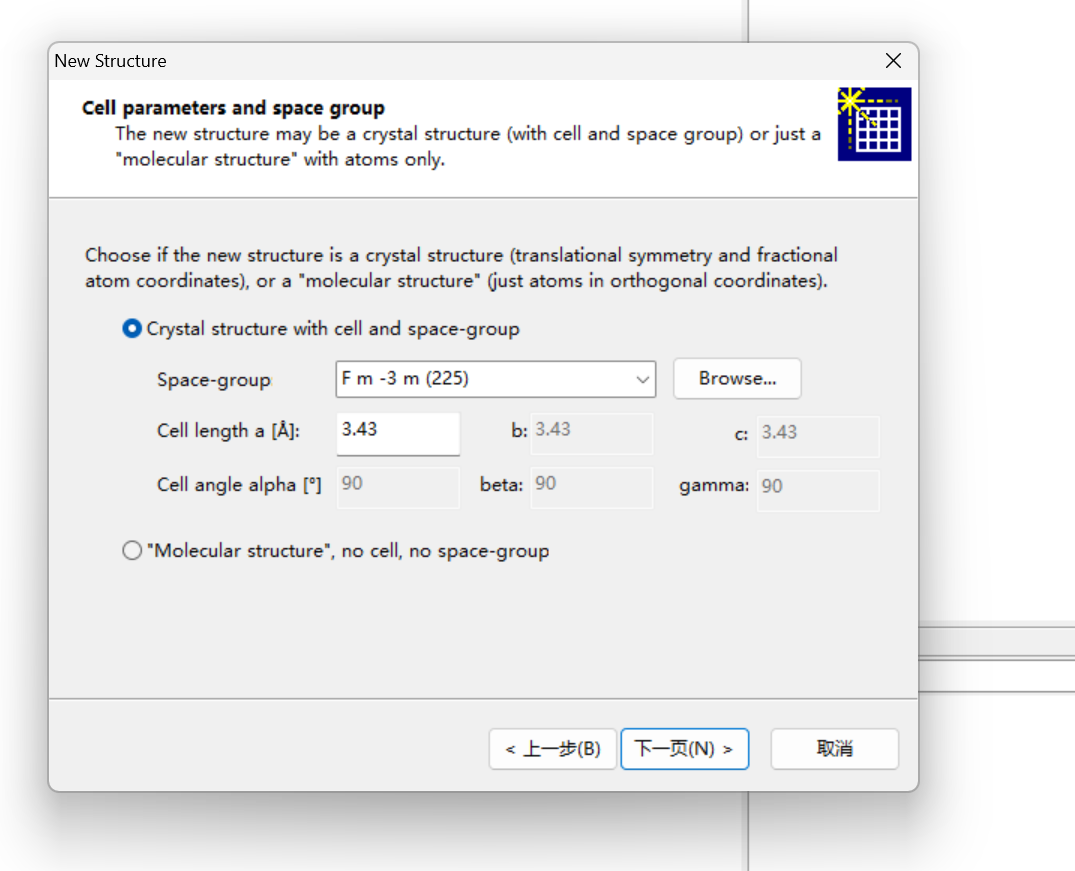
\includegraphics[width=0.44\textwidth]{assets/fcc/a.png}}
  \hfill
  \subcaptionbox{非对称单元原子（Fe）添加}{%
    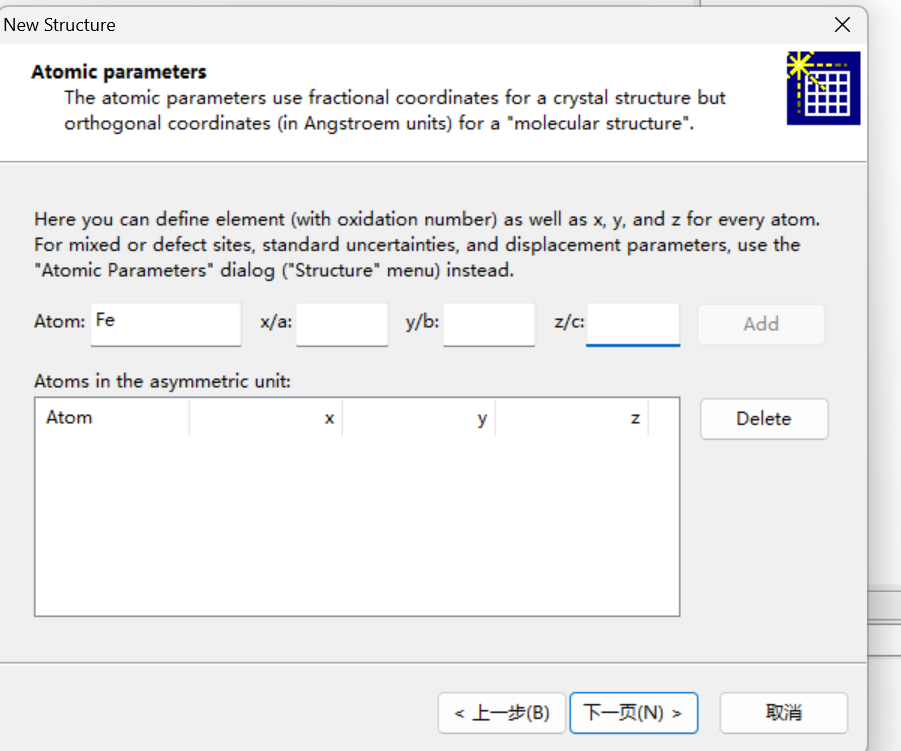
\includegraphics[width=0.44\textwidth]{assets/fcc/b.png}}
  \caption{面心立方（FCC）结构的参数设置}
  \label{fig:fcc-param}
\end{figure}

\begin{figure}[H]
  \centering
  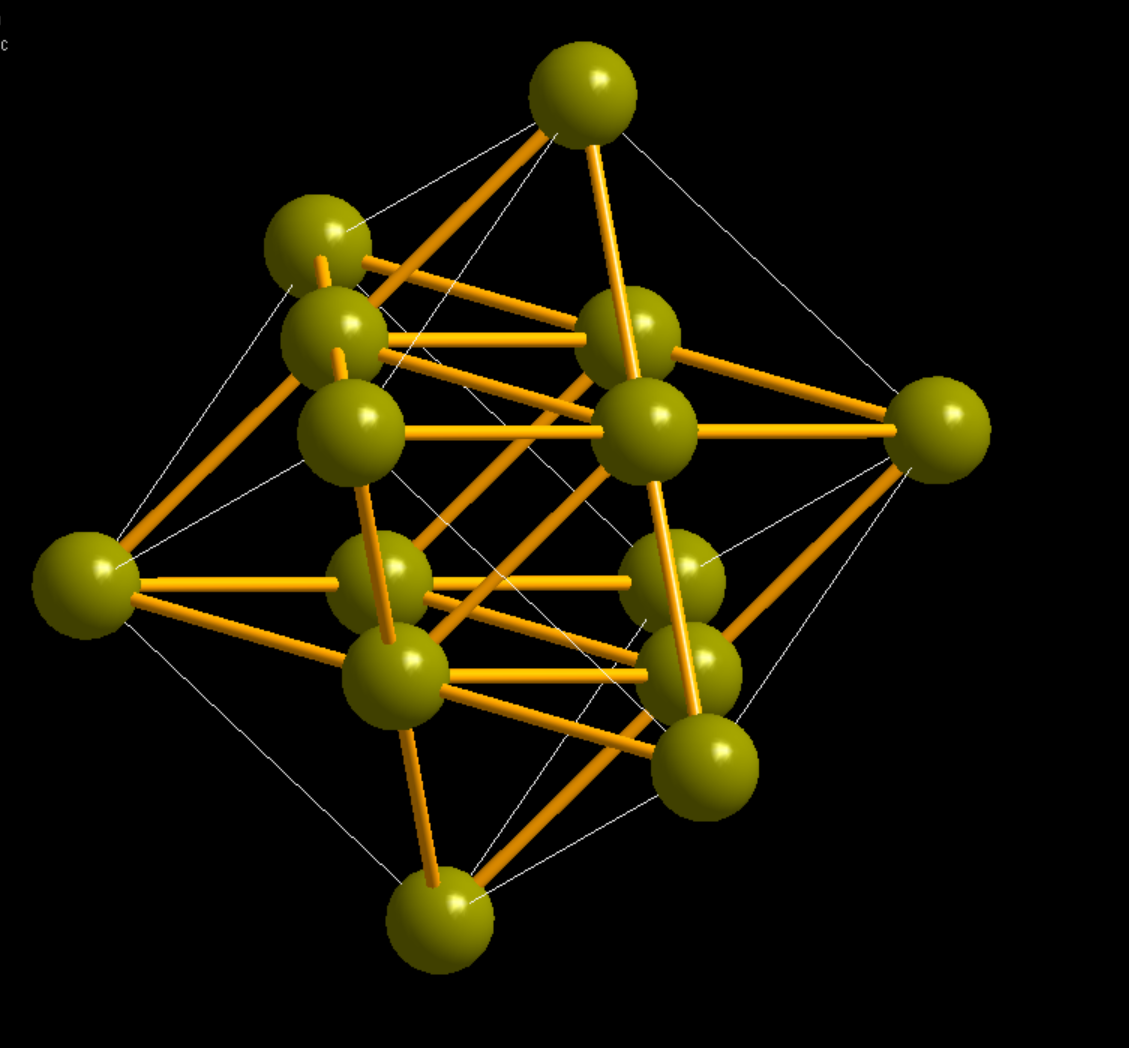
\includegraphics[width=0.5\textwidth]{assets/fcc/c.png}
  \caption{面心立方（FCC）结构的晶体结构模型}
  \label{fig:fcc-model}
\end{figure}

\begin{figure}[H]
  \centering
  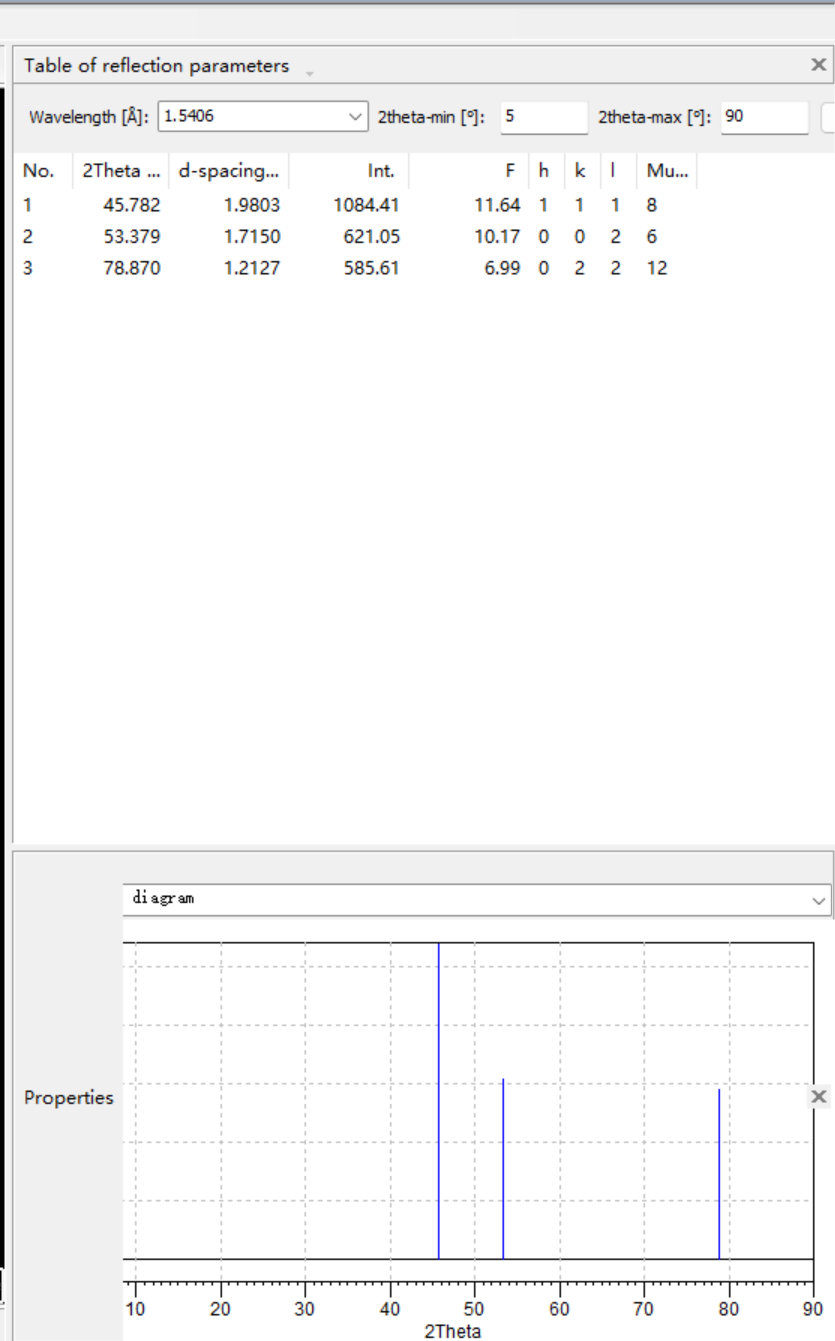
\includegraphics[width=0.4\textwidth]{assets/fcc/d.png}
  \caption{Diamond 模拟的面心立方（FCC）结构粉末衍射图}
  \label{fig:fcc-xrd}
\end{figure}

\begin{figure}[H]
  \centering
  \subcaptionbox{$\{111\}$ 密排面视图}{%
    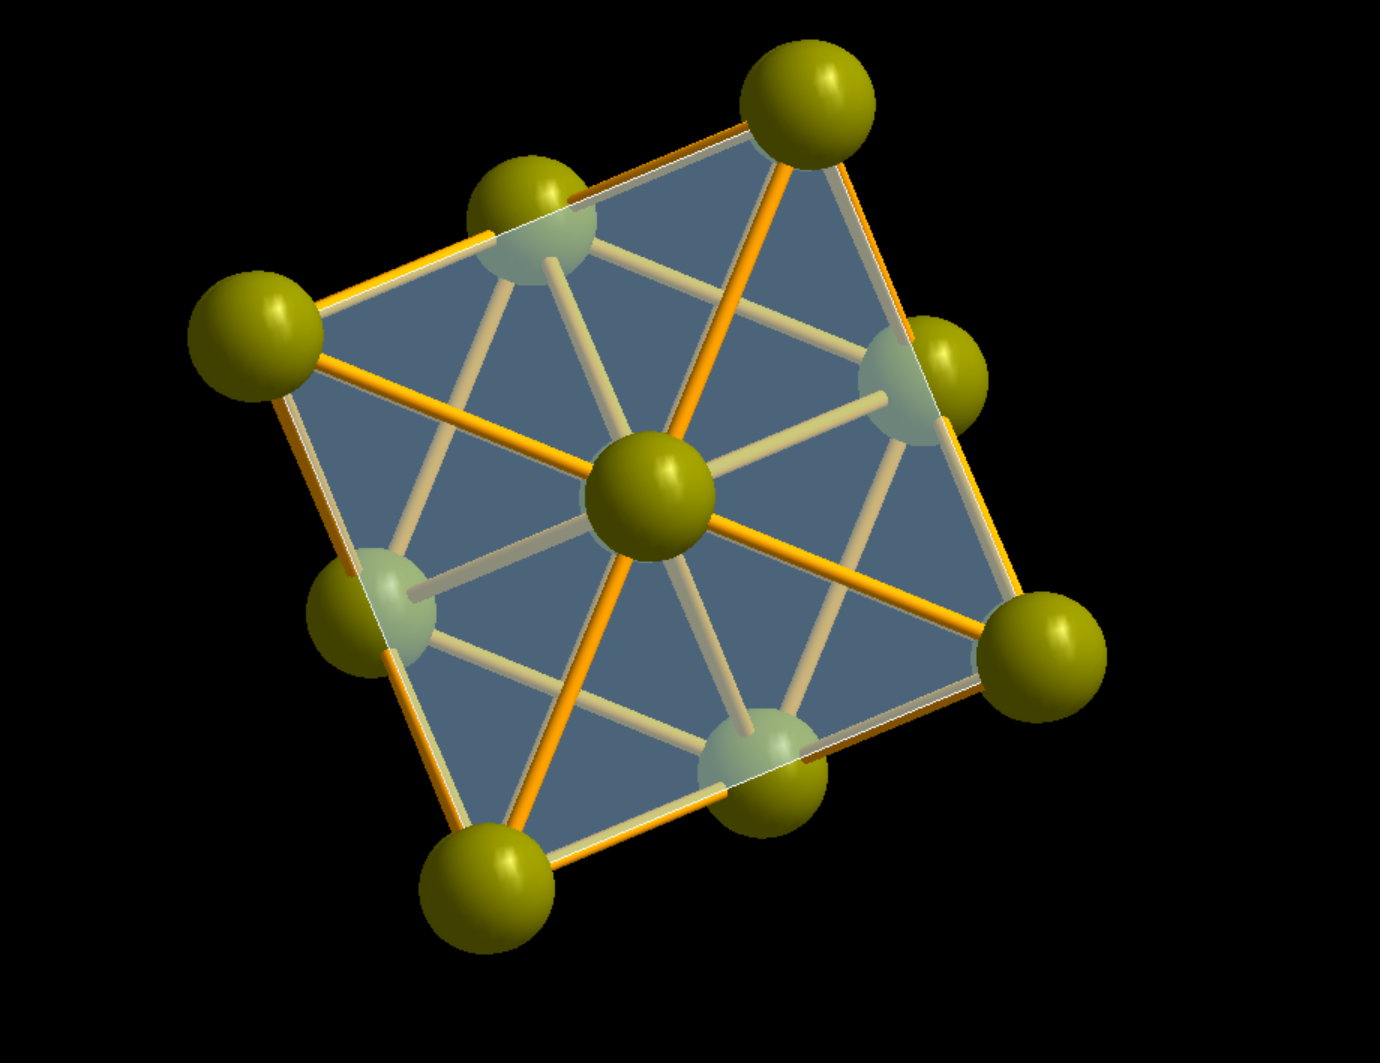
\includegraphics[width=0.46\textwidth]{assets/fcc/e.png}}
  \hfill
  \subcaptionbox{最近邻配位多面体（配位数 12）}{%
    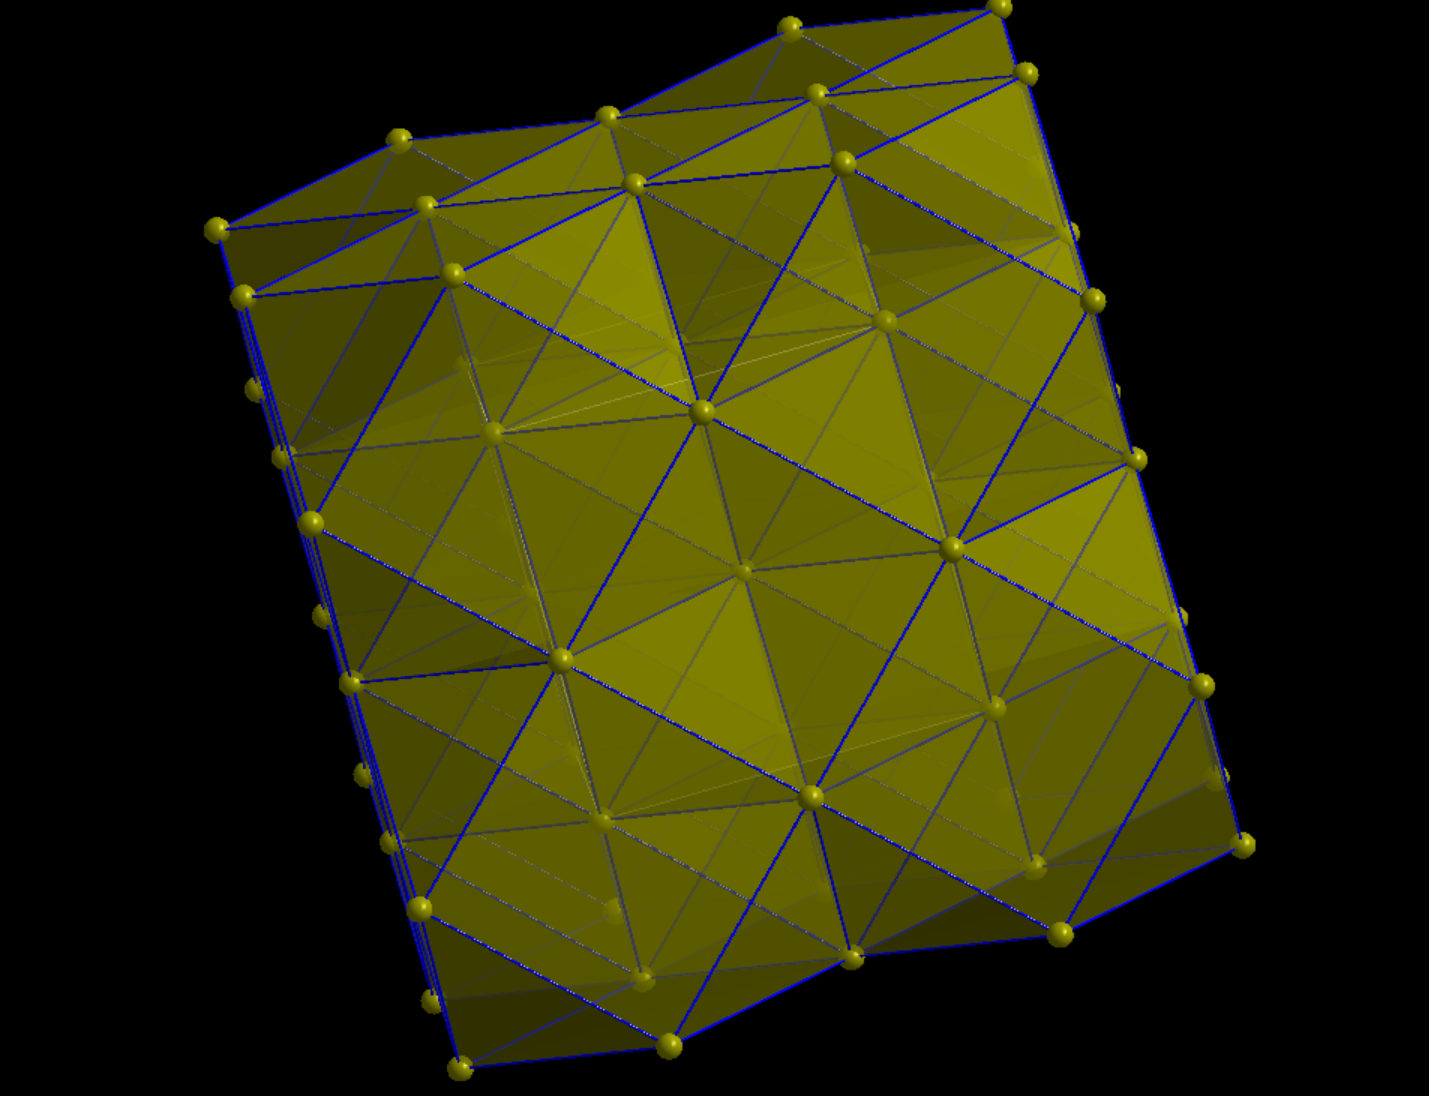
\includegraphics[width=0.44\textwidth]{assets/fcc/f.png}}
  \caption{面心立方（FCC）结构的密排面与配位多面体}
  \label{fig:fcc-plane}
\end{figure}

\textbf{结构特征。}面心立方晶胞的原子位于 8 个顶点与 6 个面心：顶点各计 $1/8$、面心各计
$1/2$，折合晶胞内共 $8\times1/8+6\times1/2=4$ 个原子（图~\ref{fig:fcc-model}）。

FCC 的密排方向为面对角线方向 $\langle110\rangle$。沿面对角线，两端的面心原子与中间的
顶点原子相切，故 $4r=\sqrt{2}a$，即原子半径 $r=\sqrt{2}a/4$；代入本次建模所用的
$a=3.43$\,\AA 得 $r\approx1.21$\,\AA。每个原子的最近邻有 12 个（同层 6 个、上下层各
3 个），次近邻 6 个（沿 $\langle100\rangle$ 方向），最近邻配位多面体是立方八面体
（图~\ref{fig:fcc-plane}(b)）。把 4 个原子的体积与晶胞体积相比，得原子堆积因子
\begin{equation}
  \eta=\frac{4\times\frac{4}{3}\pi r^3}{a^3}
    =\frac{4\times\frac{4}{3}\pi\left(\frac{\sqrt{2}}{4}a\right)^3}{a^3}
    =\frac{\sqrt{2}\pi}{6}\approx0.7405
\end{equation}
与 HCP 并列为最紧密的堆积方式。密排面为 $\{111\}$ 面（图~\ref{fig:fcc-plane}(a)），
密排层沿 $\langle111\rangle$ 方向按 ABCABC 顺序交替堆积。晶胞内的间隙同样可以清点：
八面体间隙 4 个，位于体心 $(1/2,1/2,1/2)$ 及各棱中点；四面体间隙 8 个，如
$(1/4,1/4,1/4)$。

在 $F\,m\,\bar3\,m$ 这一符号里，$F$ 表示面心点阵，后面三个特征方向依次对应 [100] 的
镜面 $m$、[111] 的旋转反演轴 $\bar3$（立方晶系的标志）和 [110] 的镜面 $m$。Cu、Ag、Au、
Al、Ni 与 $\gamma$-Fe 都具有 FCC 结构，NaCl、金刚石等结构也以 FCC 点阵为基础。

% ==================== 2.3.2.2 BCC ====================
\jiegou{2.3.2.2}{体心立方结构（BCC）}

体心立方（BCC）的演示对象是 $\alpha$-Fe，空间群与晶格常数等输入值见表~\ref{tab:bcc}。

\begin{table}[H]
  \centering
  \caption{体心立方（BCC）结构的建模参数}
  \label{tab:bcc}
  \begin{tabular}{ll}
    \toprule
    项目 & 参数 \\
    \midrule
    空间群 & $I\,m\,\bar3\,m$（No.~229） \\
    晶格常数 & $a=b=c=2.819$\,\AA，$\alpha=\beta=\gamma=90^\circ$ \\
    原子坐标 & Fe：$(0,0,0)$（$2a$ 位） \\
    化学式单元数 & $Z=2$ \\
    \bottomrule
  \end{tabular}
\end{table}

\begin{figure}[H]
  \centering
  \subcaptionbox{空间群与晶格常数设置}{%
    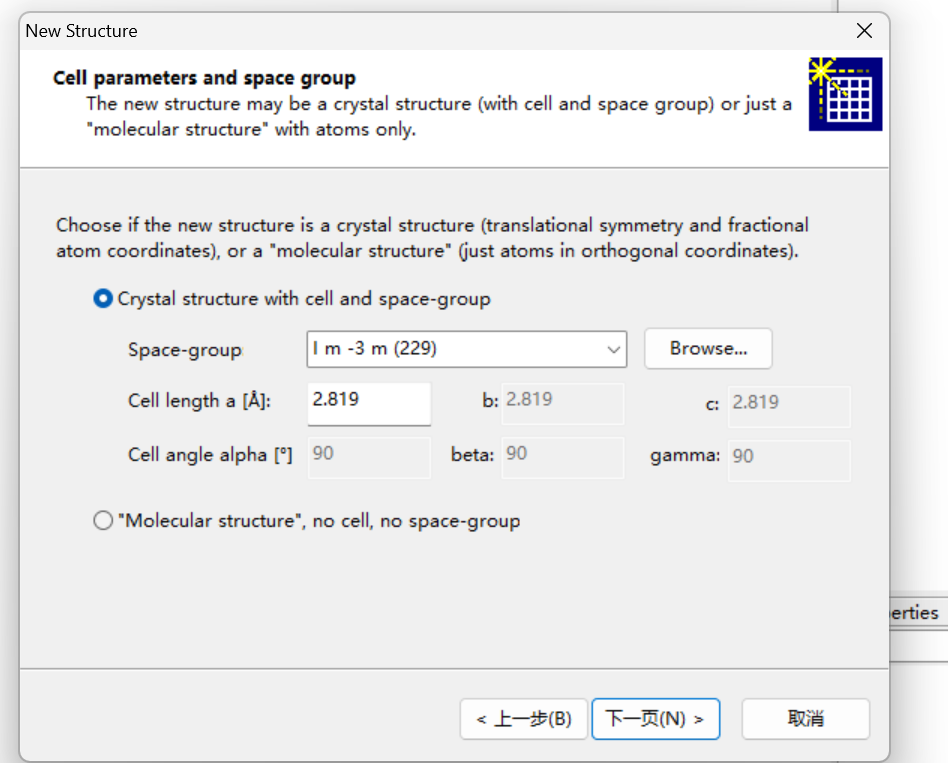
\includegraphics[width=0.44\textwidth]{assets/bcc/a.png}}
  \hfill
  \subcaptionbox{非对称单元原子（Fe）添加}{%
    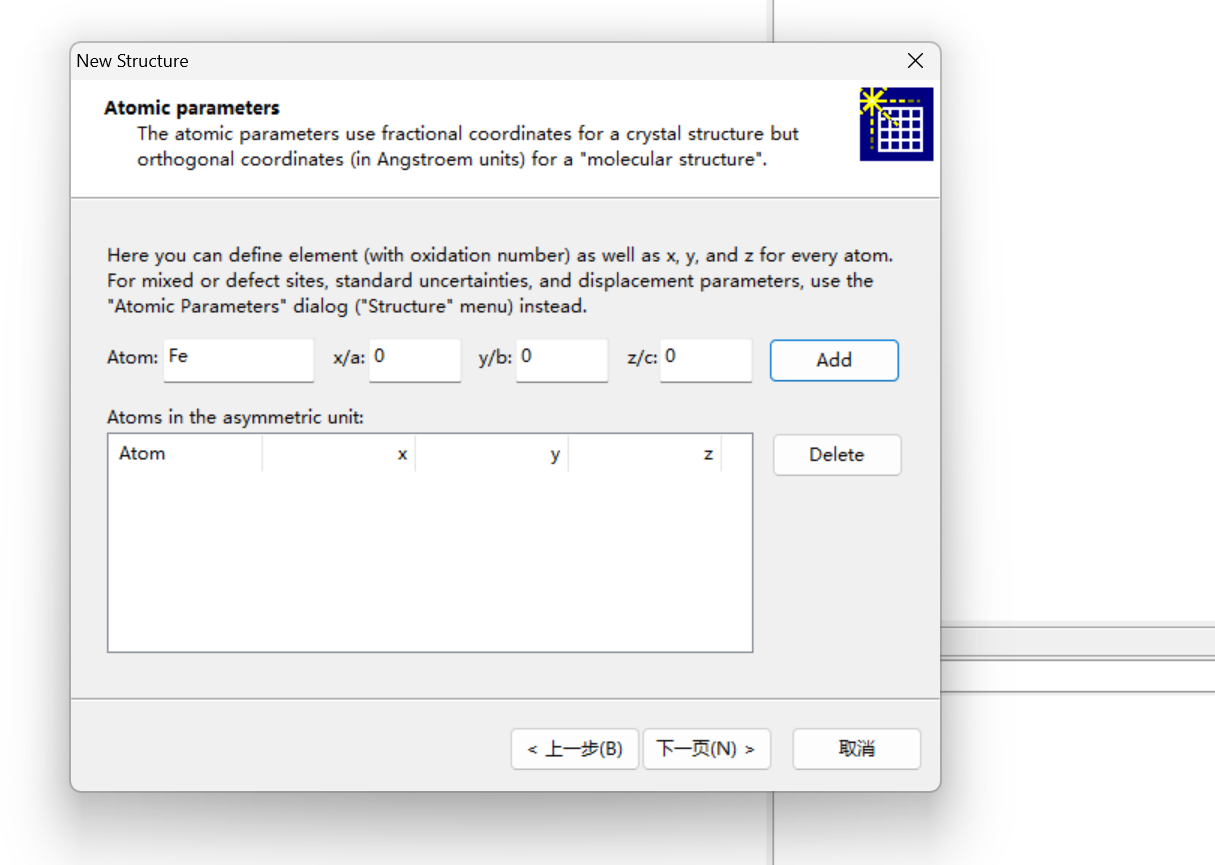
\includegraphics[width=0.44\textwidth]{assets/bcc/b.png}}
  \caption{体心立方（BCC）结构的参数设置}
  \label{fig:bcc-param}
\end{figure}

\begin{figure}[H]
  \centering
  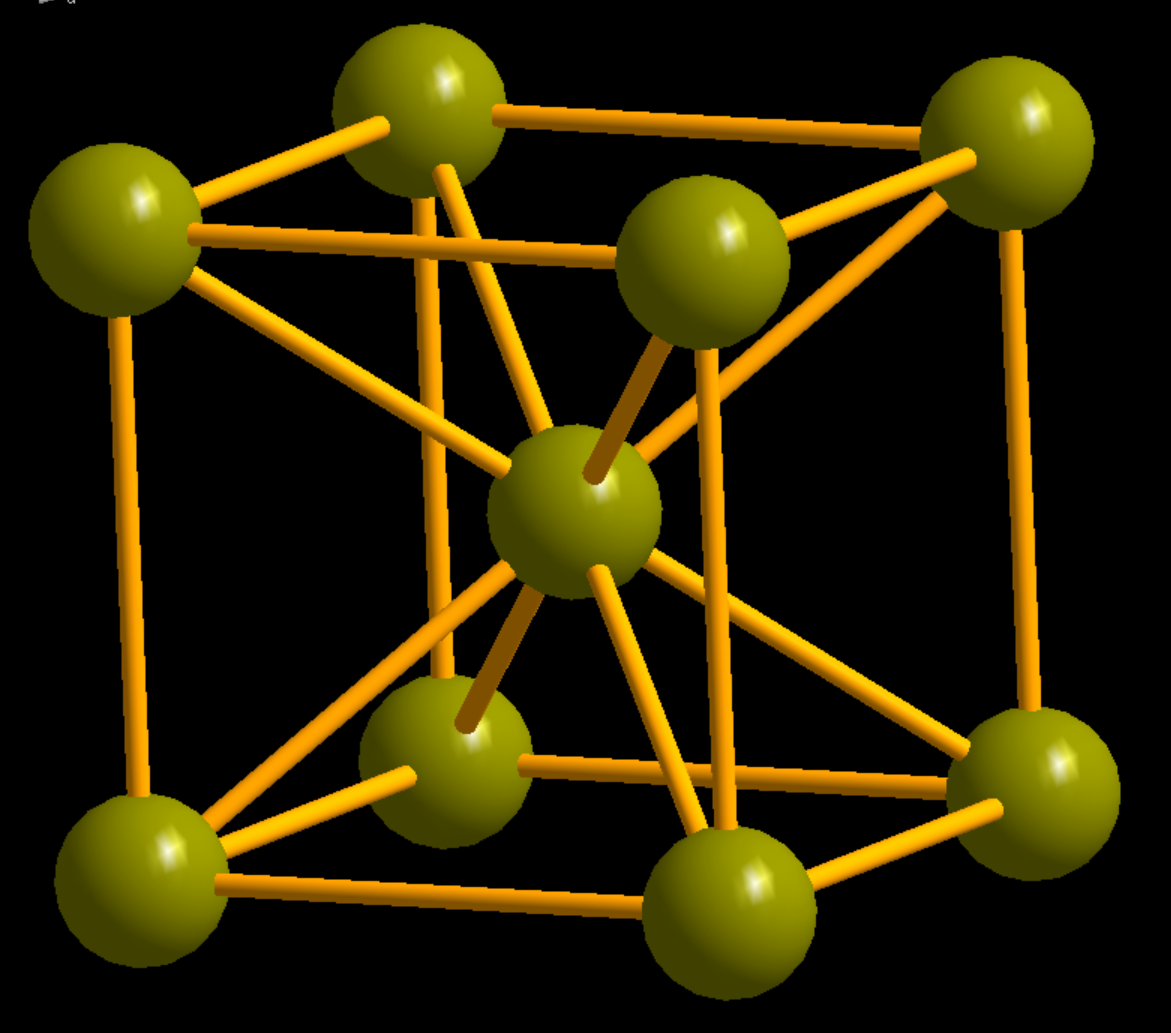
\includegraphics[width=0.5\textwidth]{assets/bcc/c.png}
  \caption{体心立方（BCC）结构的晶体结构模型}
  \label{fig:bcc-model}
\end{figure}

\begin{figure}[H]
  \centering
  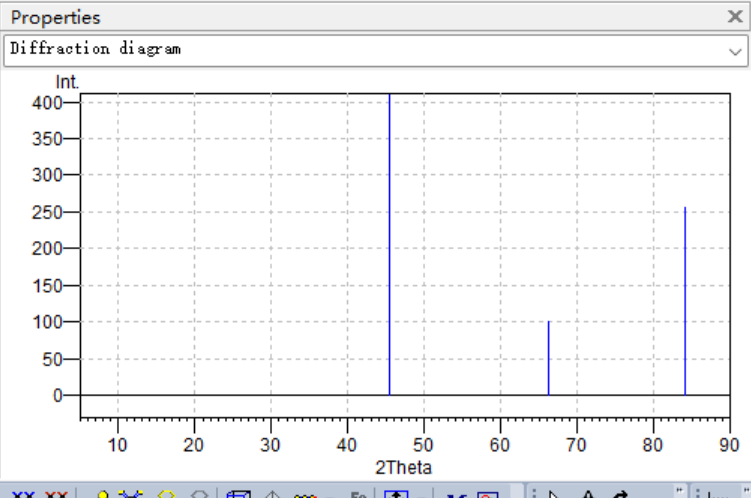
\includegraphics[width=0.5\textwidth]{assets/bcc/d.png}
  \caption{Diamond 模拟的体心立方（BCC）结构粉末衍射图}
  \label{fig:bcc-xrd}
\end{figure}

\begin{figure}[H]
  \centering
  \subcaptionbox{(111) 晶面视图}{%
    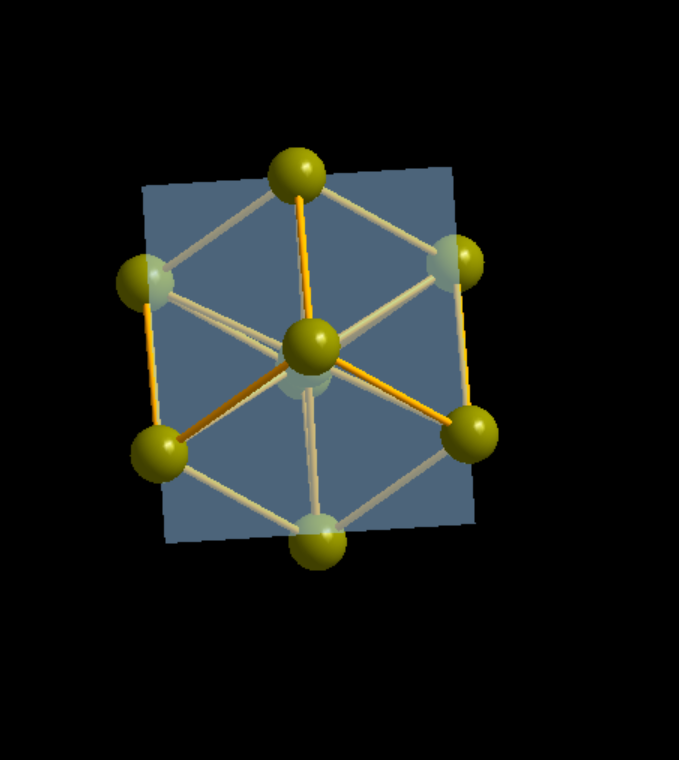
\includegraphics[width=0.44\textwidth]{assets/bcc/e.png}}
  \hfill
  \subcaptionbox{最近邻配位多面体（配位数 8）}{%
    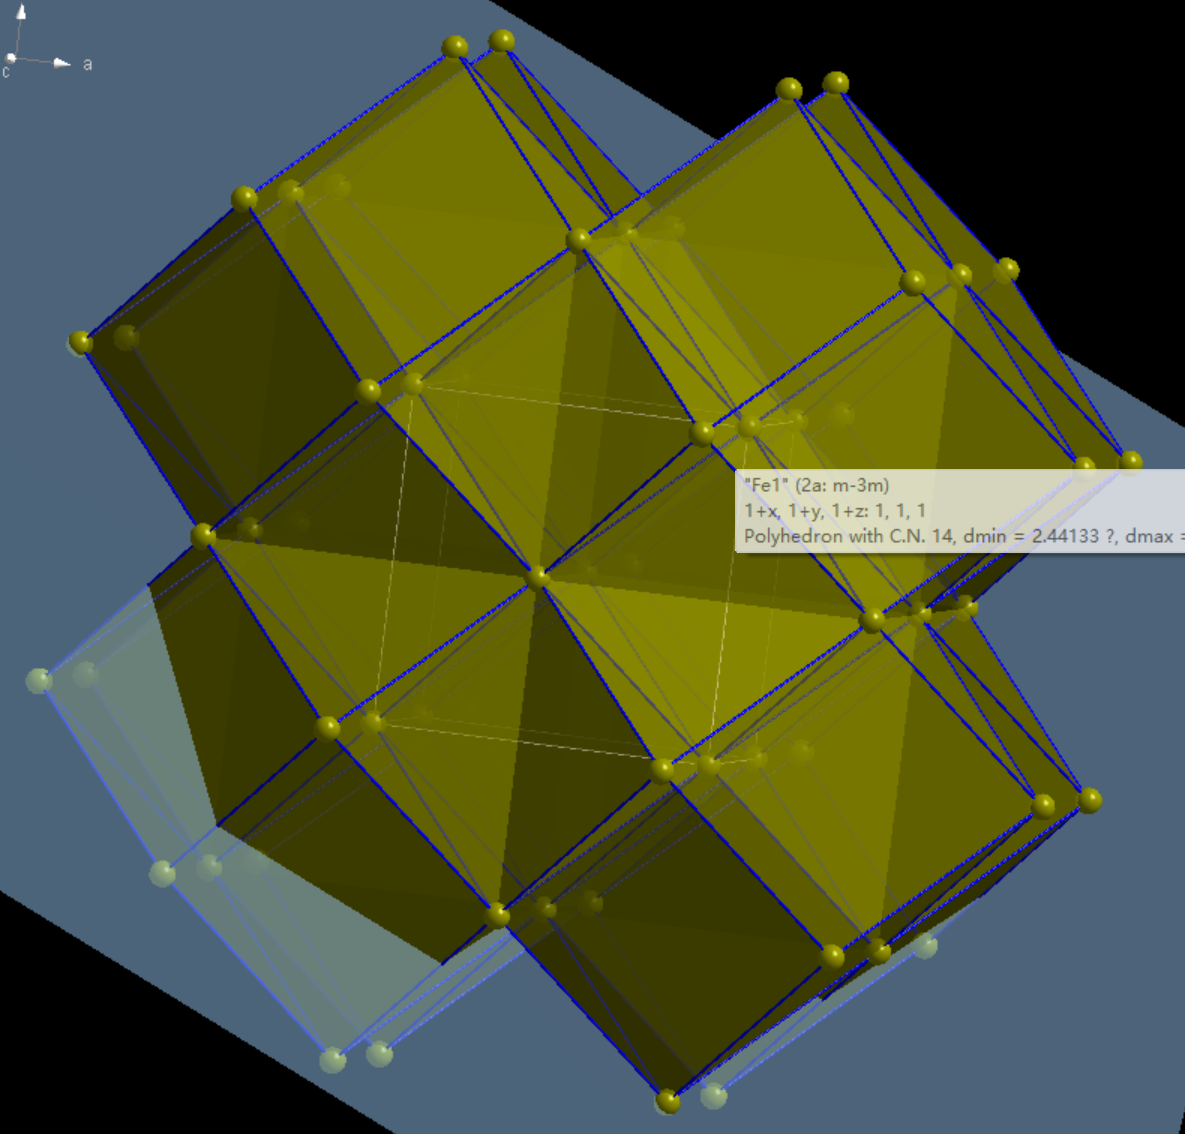
\includegraphics[width=0.46\textwidth]{assets/bcc/f.png}}
  \caption{体心立方（BCC）结构的晶面与配位多面体}
  \label{fig:bcc-plane}
\end{figure}

\textbf{结构特征。}顶点 8 个原子各计 $1/8$，再加上体心的 1 个，晶胞内共 2 个原子；
体心原子与 8 个顶点原子等距（图~\ref{fig:bcc-model}）。

沿体对角线方向，体心原子与两端的顶点原子相切，故 $4r=\sqrt{3}a$，$r=\sqrt{3}a/4$；
代入 $a=2.819$\,\AA 得 $r\approx1.22$\,\AA。最近邻 8 个，配位多面体为立方体
（图~\ref{fig:bcc-plane}(b)）；次近邻 6 个，位于 $\langle100\rangle$ 方向的相邻晶胞
体心。堆积因子为
\begin{equation}
  \eta=\frac{2\times\frac{4}{3}\pi r^3}{a^3}
    =\frac{2\times\frac{4}{3}\pi\left(\frac{\sqrt{3}}{4}a\right)^3}{a^3}
    =\frac{\sqrt{3}\pi}{8}\approx0.6802
\end{equation}
明显低于 FCC 与 HCP，$\alpha$-Fe 在相变（如马氏体相变）中伴随的体积变化正与此有关。
BCC 没有严格意义上的密排面，面间距最大的 $\{110\}$ 面可视为``最密''面；
图~\ref{fig:bcc-plane}(a) 演示的是在模型中添加 (111) 晶面（$d_{111}=1.6276$\,\AA）
后的观察效果。

$I\,m\,\bar3\,m$ 中的 $I$ 代表体心点阵，其余符号的含义与 FCC 相同。Cr、Mo、W、V 以及
碱金属 Na、K 等都是 BCC 结构，$\alpha$-Fe 是其中最熟悉的例子。

% ==================== 2.3.2.3 HCP ====================
\jiegou{2.3.2.3}{六方密堆积结构（HCP）}

以镁为例建立六方密堆积结构模型，建模参数见表~\ref{tab:hcp}。六方晶系以 $a$、$b$ 轴
夹角 $120^\circ$ 为特征，HCP 结构的非对称单元含有两个不等价原子。

\begin{table}[H]
  \centering
  \caption{六方密堆积（HCP）结构的建模参数}
  \label{tab:hcp}
  \begin{tabular}{ll}
    \toprule
    项目 & 参数 \\
    \midrule
    空间群 & $P\,6_3/m\,m\,c$（No.~194） \\
    晶格常数 & $a=b=3.2085$\,\AA，$c=5.2106$\,\AA，$\alpha=\beta=90^\circ$，
      $\gamma=120^\circ$ \\
    原子坐标 & Mg：$(0,0,0)$、$(1/3,2/3,1/2)$（$2c$ 位） \\
    化学式单元数 & $Z=2$ \\
    \bottomrule
  \end{tabular}
\end{table}

\begin{figure}[H]
  \centering
  \subcaptionbox{空间群与晶格常数设置}{%
    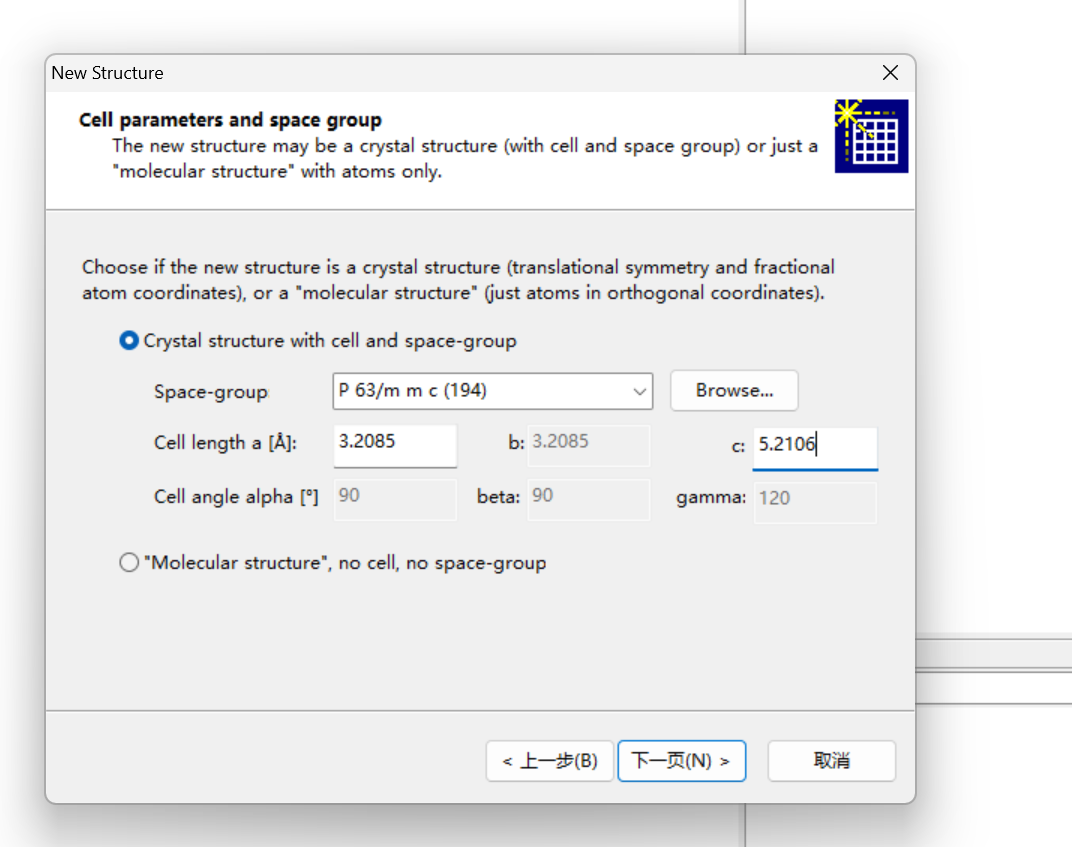
\includegraphics[width=0.44\textwidth]{assets/hcp/a.png}}
  \hfill
  \subcaptionbox{非对称单元原子（Mg）添加}{%
    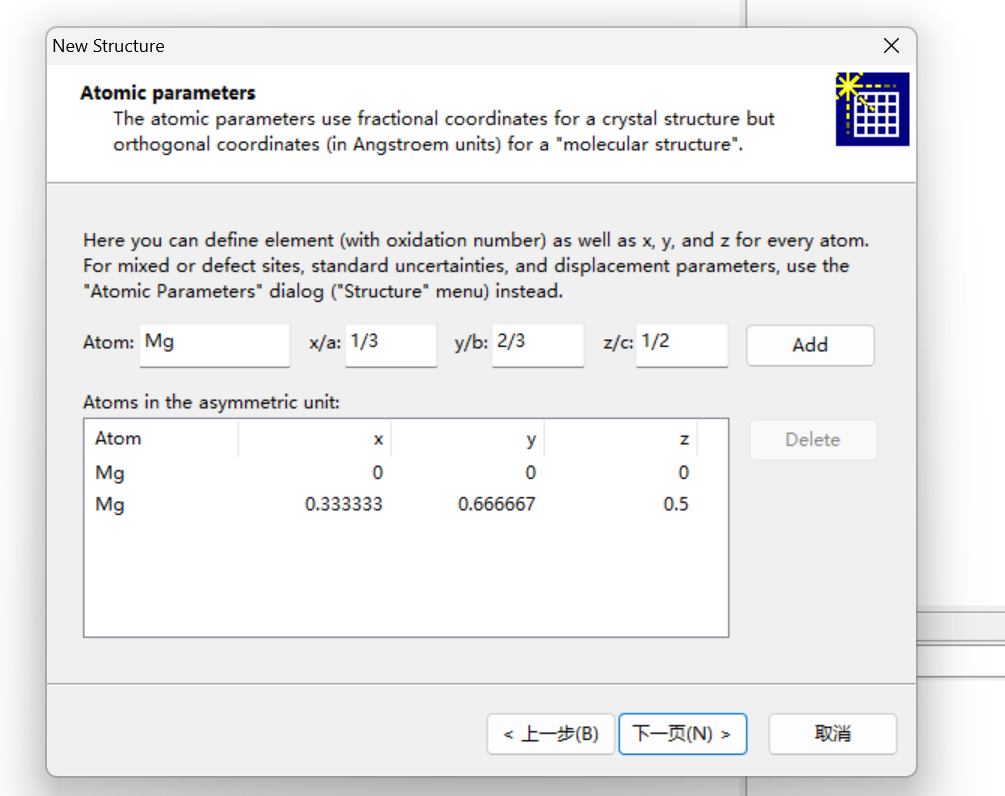
\includegraphics[width=0.44\textwidth]{assets/hcp/b.png}}
  \caption{六方密堆积（HCP）结构的参数设置}
  \label{fig:hcp-param}
\end{figure}

\begin{figure}[H]
  \centering
  \subcaptionbox{结构模型（视角一）}{%
    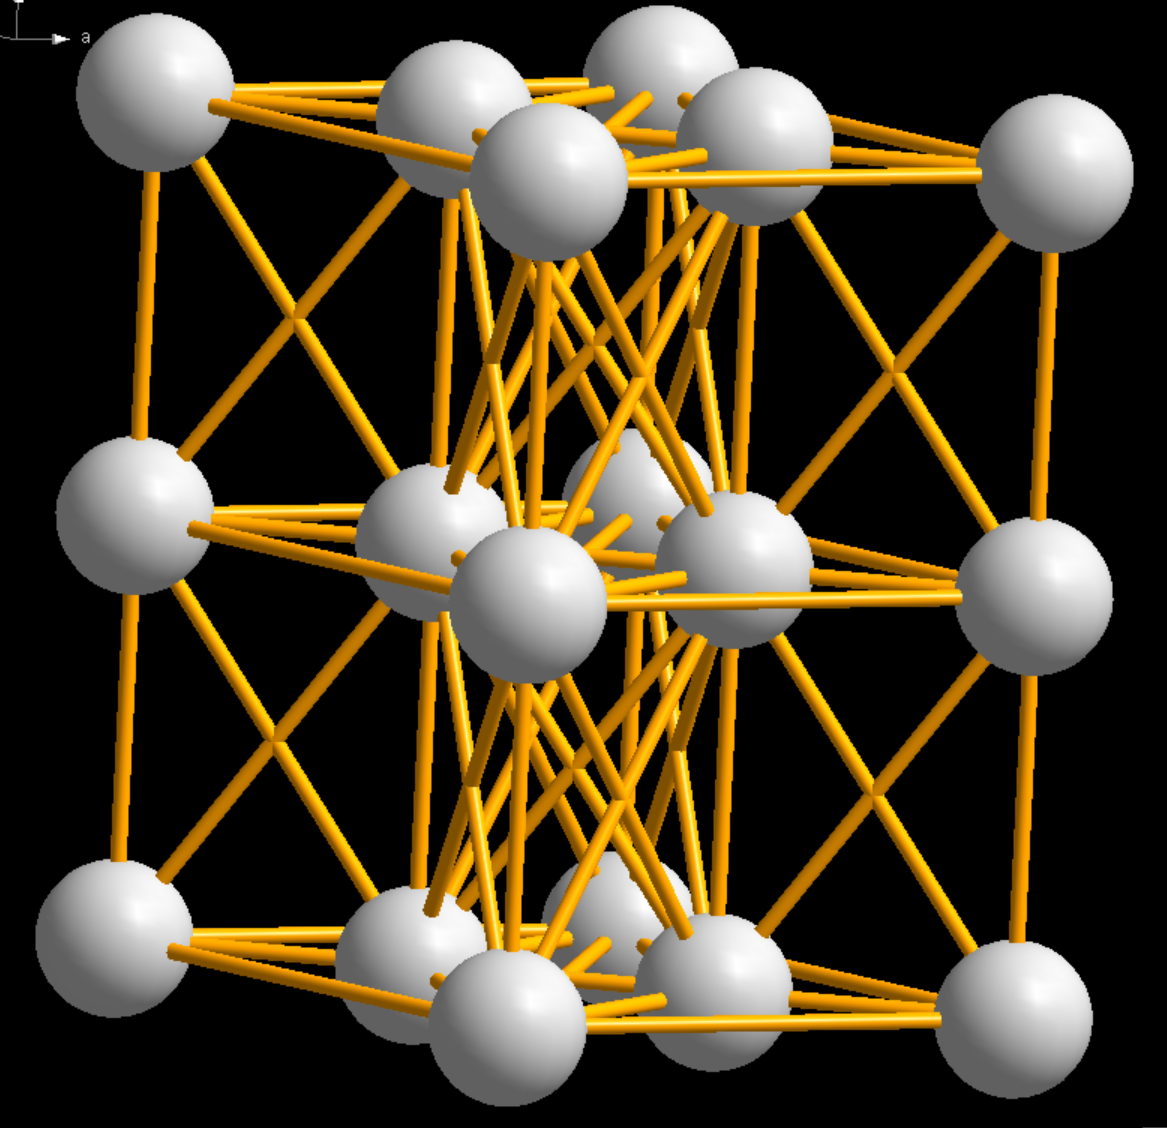
\includegraphics[width=0.44\textwidth]{assets/hcp/c.png}}
  \hfill
  \subcaptionbox{结构模型（视角二）}{%
    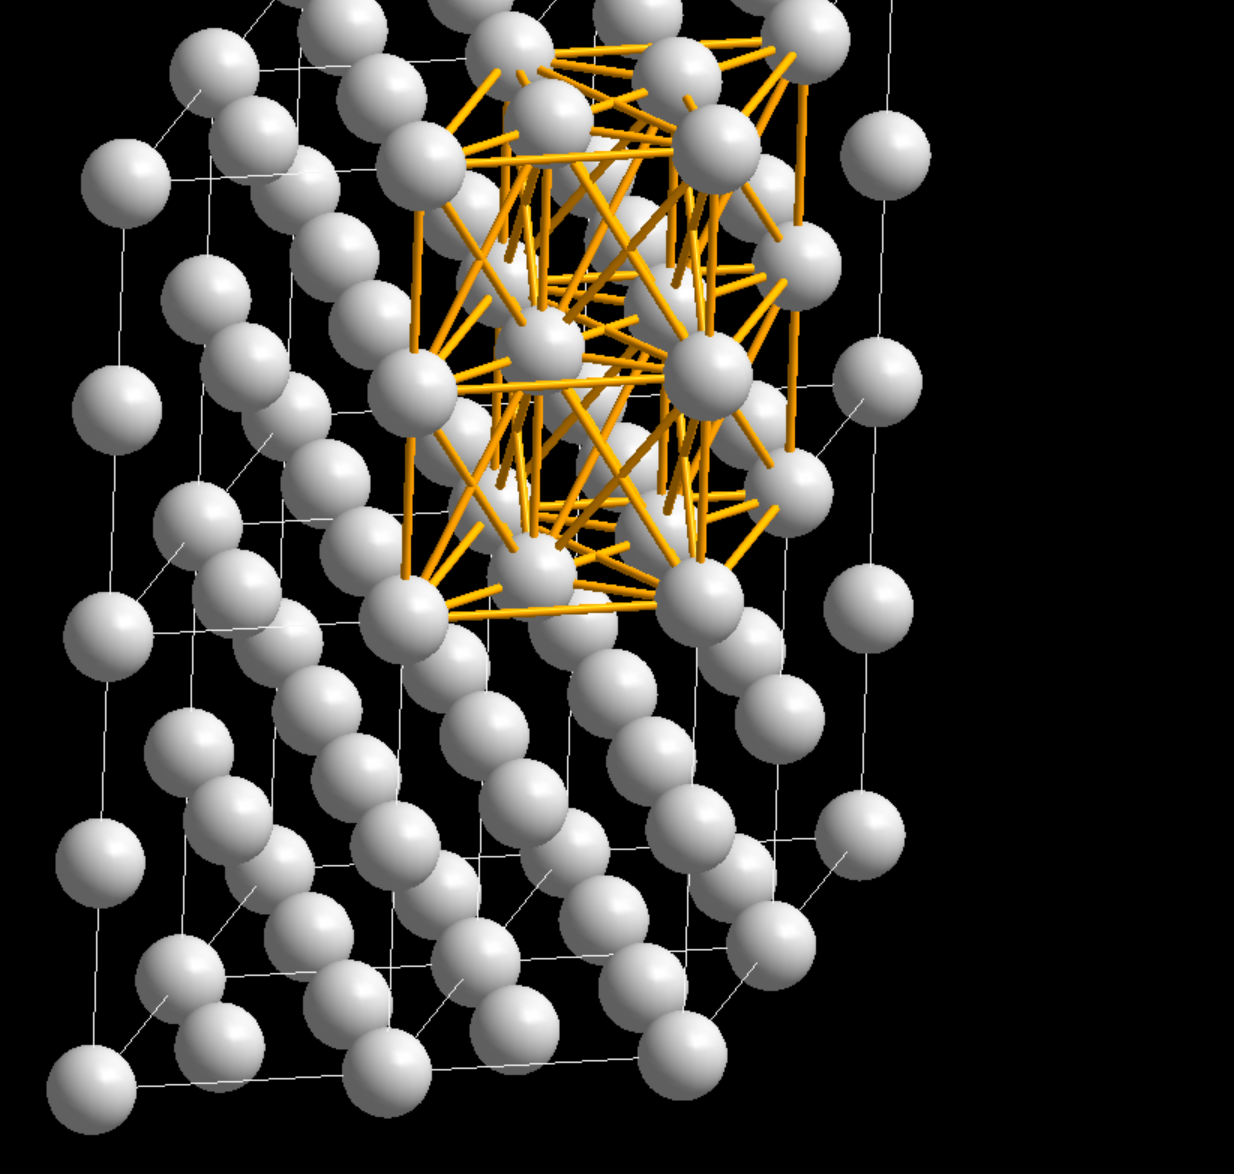
\includegraphics[width=0.44\textwidth]{assets/hcp/extra.png}}
  \caption{六方密堆积（HCP）结构的晶体结构模型}
  \label{fig:hcp-model}
\end{figure}

\begin{figure}[H]
  \centering
  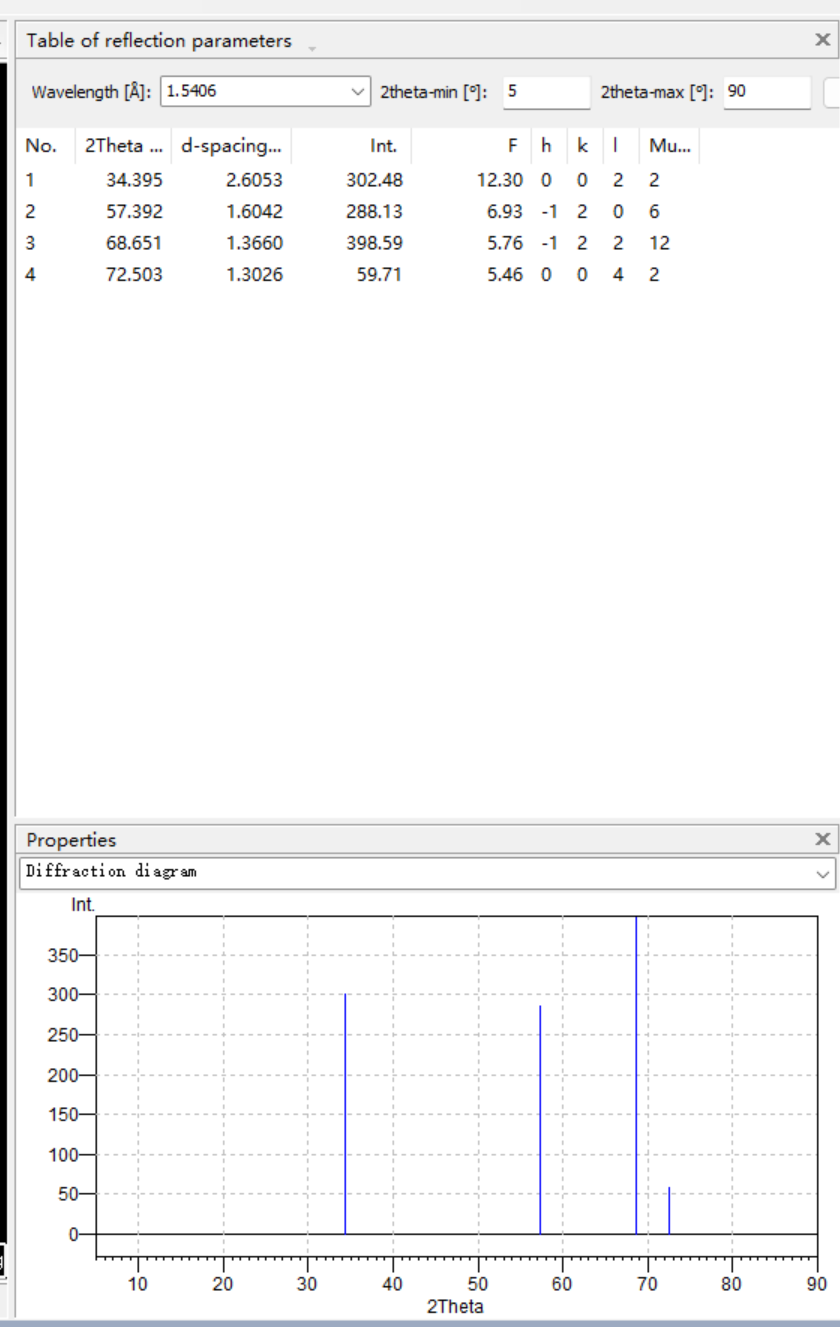
\includegraphics[width=0.4\textwidth]{assets/hcp/d.png}
  \caption{Diamond 模拟的六方密堆积（HCP）结构粉末衍射图}
  \label{fig:hcp-xrd}
\end{figure}

\begin{figure}[H]
  \centering
  \subcaptionbox{$(0001)$ 密排面（基面）视图}{%
    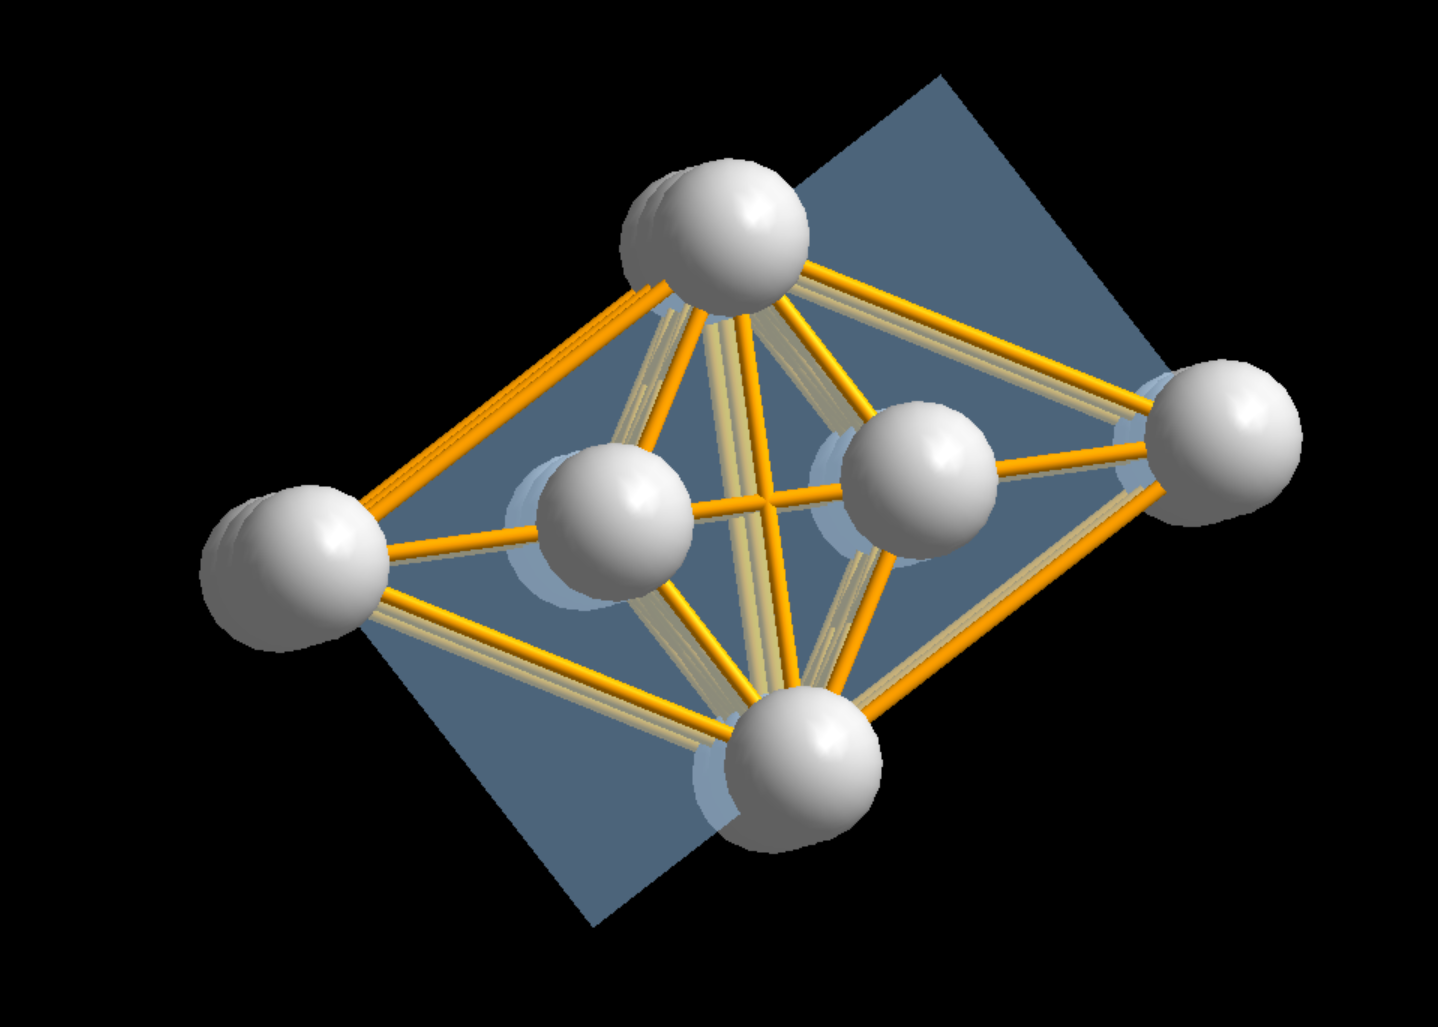
\includegraphics[width=0.46\textwidth]{assets/hcp/e.png}}
  \hfill
  \subcaptionbox{最近邻配位多面体（配位数 12）}{%
    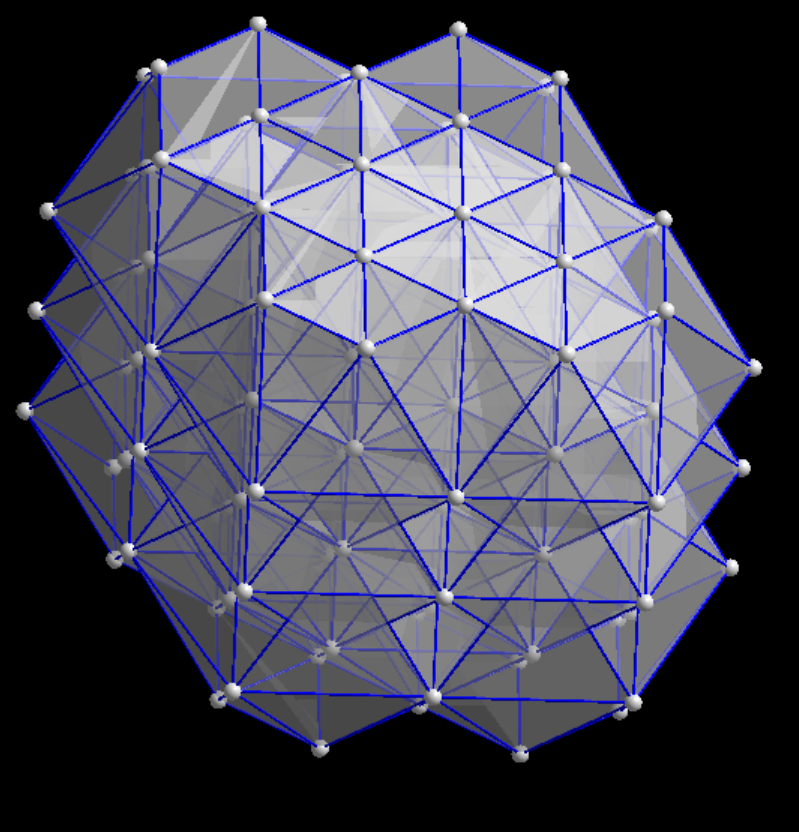
\includegraphics[width=0.44\textwidth]{assets/hcp/f.png}}
  \caption{六方密堆积（HCP）结构的密排面与配位多面体}
  \label{fig:hcp-plane}
\end{figure}

\textbf{结构特征。}HCP 晶胞的两个原子分别位于 $(0,0,0)$ 与 $(1/3,2/3,1/2)$，晶胞内
原子数为 2。与 FCC 一样，HCP 也是原子最紧密堆积方式之一，两者堆积因子相同，但堆积
顺序不同。

\begin{enumerate}[label=（\arabic*）]
  \item \textbf{轴比}：本模型的轴比 $c/a=5.2106/3.2085\approx1.624$，略小于刚球密
    堆积的理想值 $c/a=\sqrt{8/3}\approx1.633$。轴比的偏离意味着层间原子不完全按刚球
    相切排列，实际金属（Mg、Zn 等）的轴比多略偏离理想值。
  \item \textbf{配位数}：每个原子有 12 个最近邻原子（同层 6 个、上下层各 3 个），
    配位多面体为六方密堆积特征的多面体（图~\ref{fig:hcp-plane}(b)）。
  \item \textbf{原子堆积因子}：在刚球模型下 $r=a/2$，晶胞体积
    $V=\dfrac{\sqrt{3}}{2}a^2c$，故
    \begin{equation}
      \eta=\frac{2\times\frac{4}{3}\pi\left(\frac{a}{2}\right)^3}
                {\frac{\sqrt{3}}{2}a^2c}
        =\frac{2\pi a}{3\sqrt{3}c}
    \end{equation}
    代入理想轴比 $c=\sqrt{8/3}\,a$ 得 $\eta=\pi/(3\sqrt{2})\approx0.7405$。
  \item \textbf{密排面与堆积方式}：密排面为 $(0001)$ 基面（图~\ref{fig:hcp-plane}(a)），
    密排层沿 $[0001]$ 方向按 ABAB 方式交替堆积；FCC 则为 ABCABC 堆积。若晶体生长过程
    中某密排层缺失，FCC 的 ABCABC 序被破坏，很容易形成 ABAB 排列，即 HCP 结构，这是
    许多材料中 FCC $\leftrightarrow$ HCP 结构相变的根源。
\end{enumerate}

空间群符号 $P\,6_3/m\,m\,c$ 表明：$P$ 为六方初基点阵，[001] 方向为 $6_3$ 螺旋轴加
镜面，[100] 方向为镜面 $m$，[120] 方向为 $c$ 滑移面。具有 HCP 结构的典型金属有 Mg、
Zn、Ti、Co 等。

% ==================== 2.3.2.4 NaCl ====================
\jiegou{2.3.2.4}{氯化钠结构（NaCl 型）}

NaCl 结构的演示对象就是 NaCl 本身，它可视作两套面心立方点阵沿 $\langle100\rangle$
方向相互平移 $(1/2,0,0)$ 嵌套而成；建模参数见表~\ref{tab:nacl}。

\begin{table}[H]
  \centering
  \caption{氯化钠（NaCl）结构的建模参数}
  \label{tab:nacl}
  \begin{tabular}{ll}
    \toprule
    项目 & 参数 \\
    \midrule
    空间群 & $F\,m\,\bar3\,m$（No.~225） \\
    晶格常数 & $a=b=c=5.62$\,\AA，$\alpha=\beta=\gamma=90^\circ$ \\
    原子坐标 & Na$^+$：$(1/2,0,0)$（$4b$ 位）；Cl$^-$：$(0,0,0)$（$4a$ 位） \\
    化学式单元数 & $Z=4$ \\
    \bottomrule
  \end{tabular}
\end{table}

\begin{figure}[H]
  \centering
  \subcaptionbox{空间群与晶格常数设置}{%
    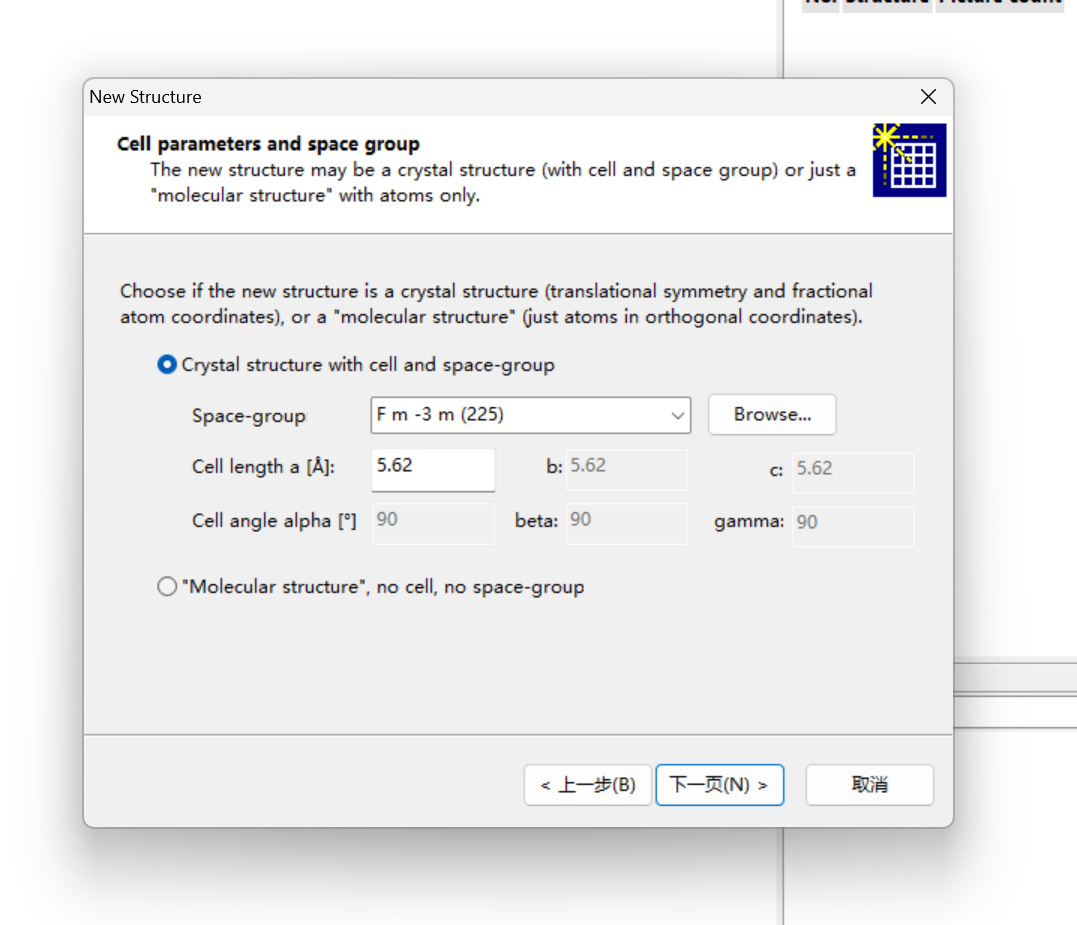
\includegraphics[width=0.44\textwidth]{assets/nacl/a.png}}
  \hfill
  \subcaptionbox{非对称单元原子（Na、Cl）添加}{%
    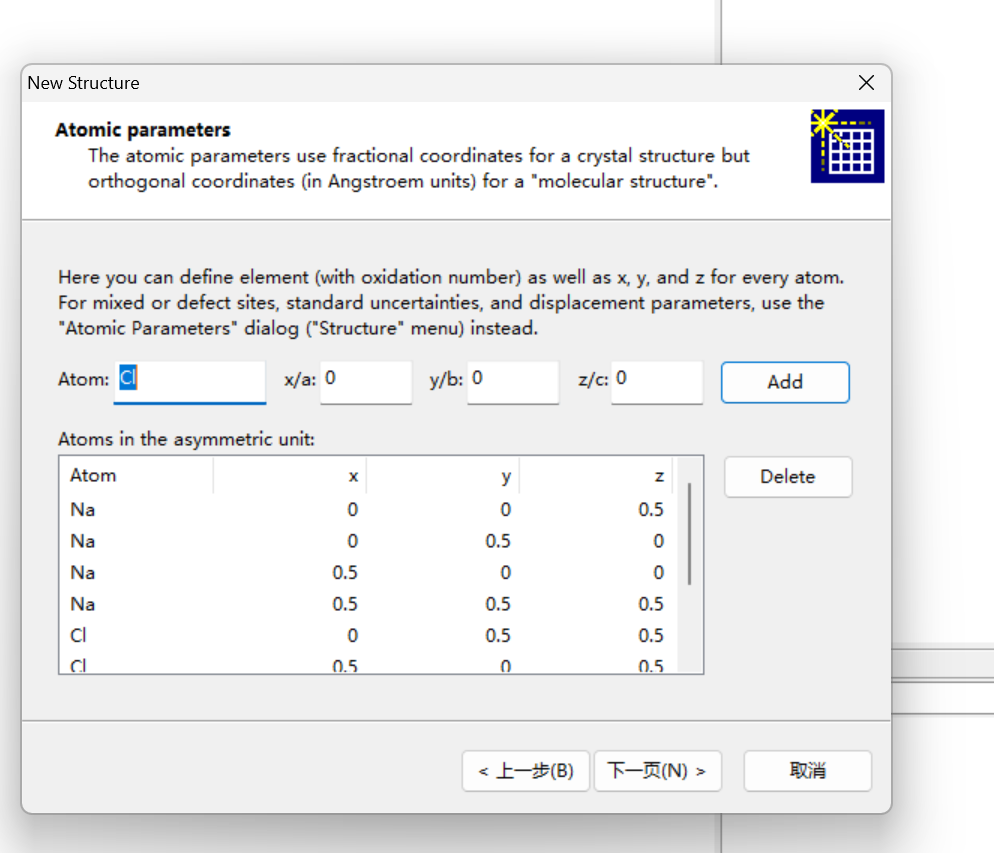
\includegraphics[width=0.44\textwidth]{assets/nacl/b.png}}
  \caption{氯化钠（NaCl）结构的参数设置}
  \label{fig:nacl-param}
\end{figure}

\begin{figure}[H]
  \centering
  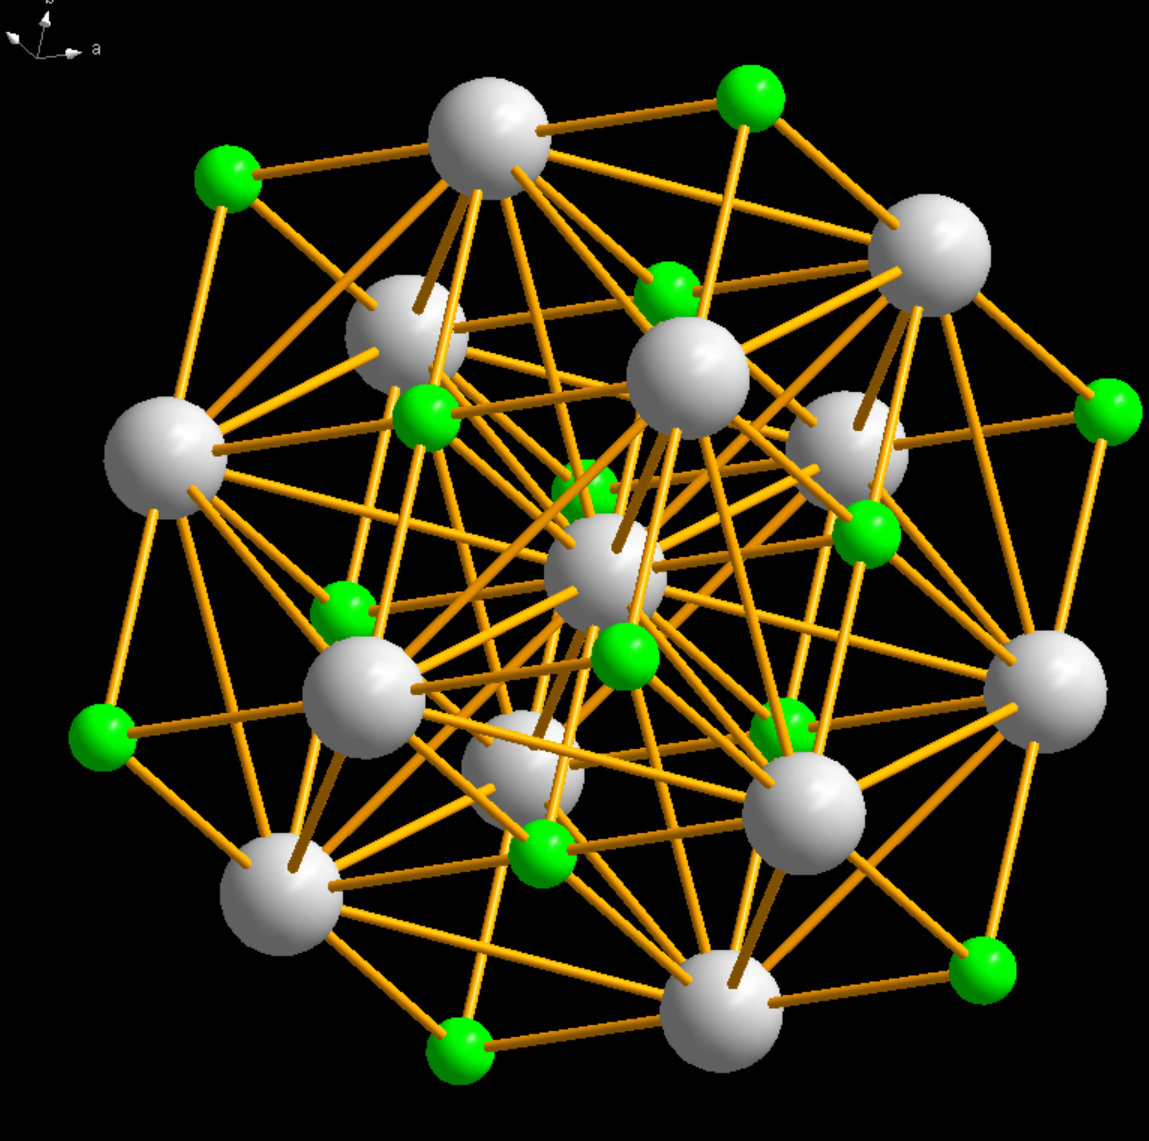
\includegraphics[width=0.5\textwidth]{assets/nacl/c.png}
  \caption{氯化钠（NaCl）结构的晶体结构模型}
  \label{fig:nacl-model}
\end{figure}

\begin{figure}[H]
  \centering
  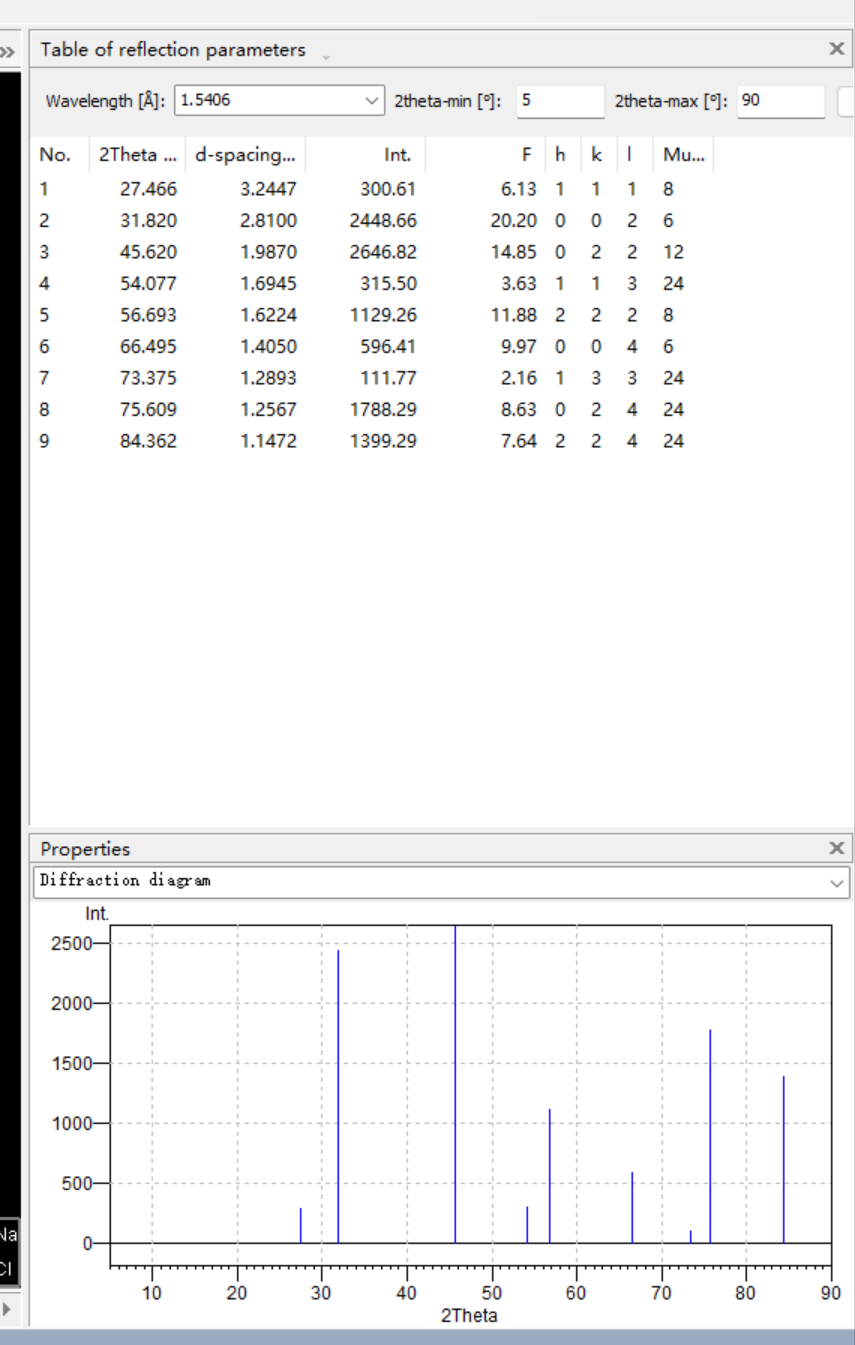
\includegraphics[width=0.4\textwidth]{assets/nacl/d.png}
  \caption{Diamond 模拟的氯化钠（NaCl）结构粉末衍射图}
  \label{fig:nacl-xrd}
\end{figure}

\begin{figure}[H]
  \centering
  \subcaptionbox{密排晶面视图}{%
    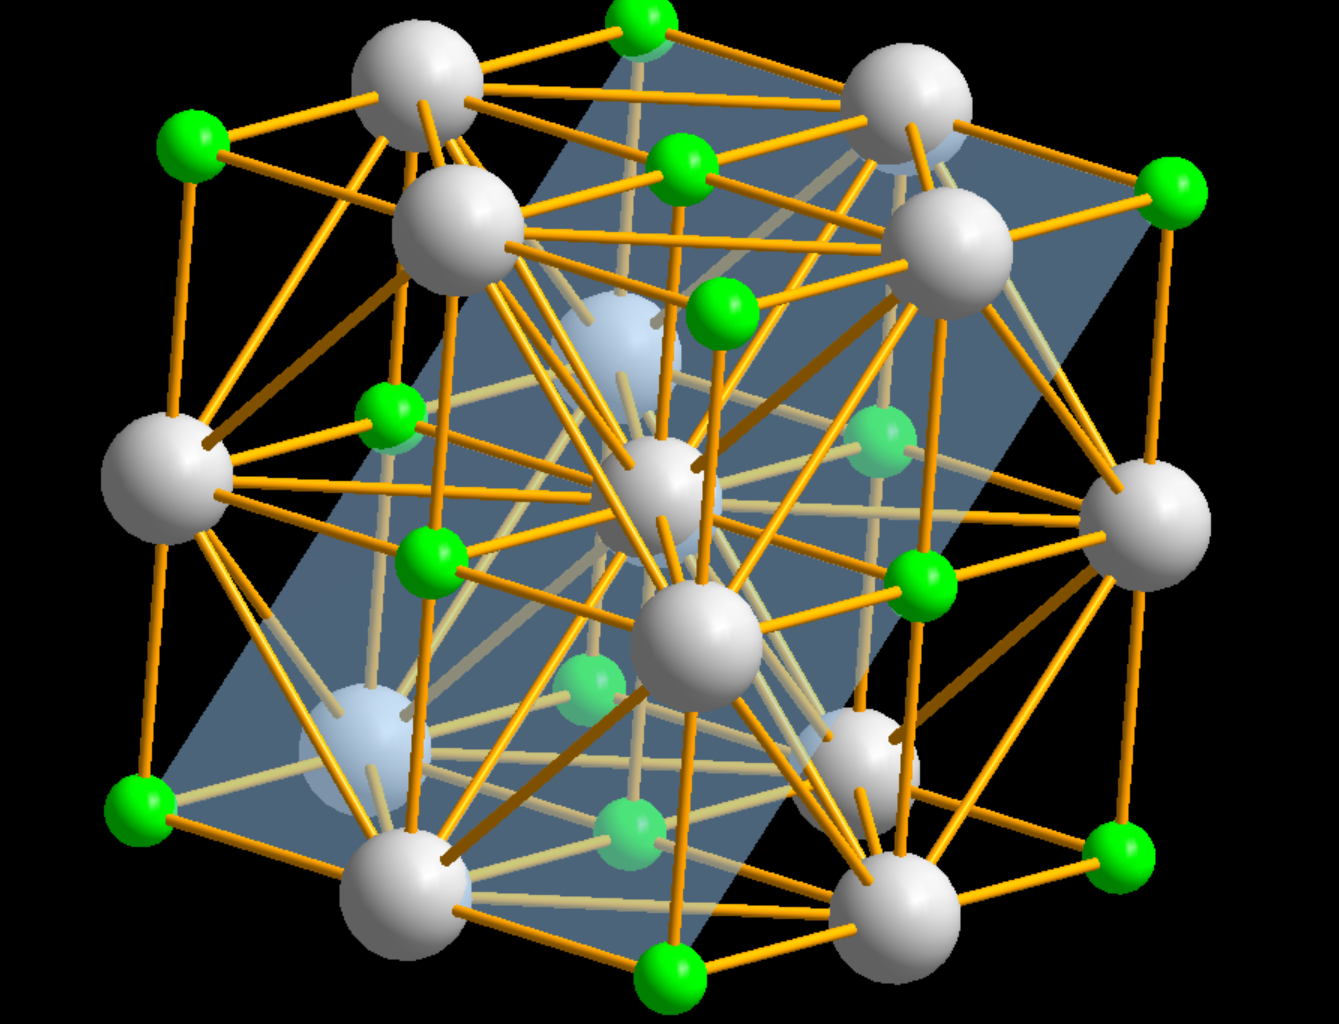
\includegraphics[width=0.40\textwidth]{assets/nacl/e.png}}
  \hfill
  \subcaptionbox{配位八面体（配位数 6）}{%
    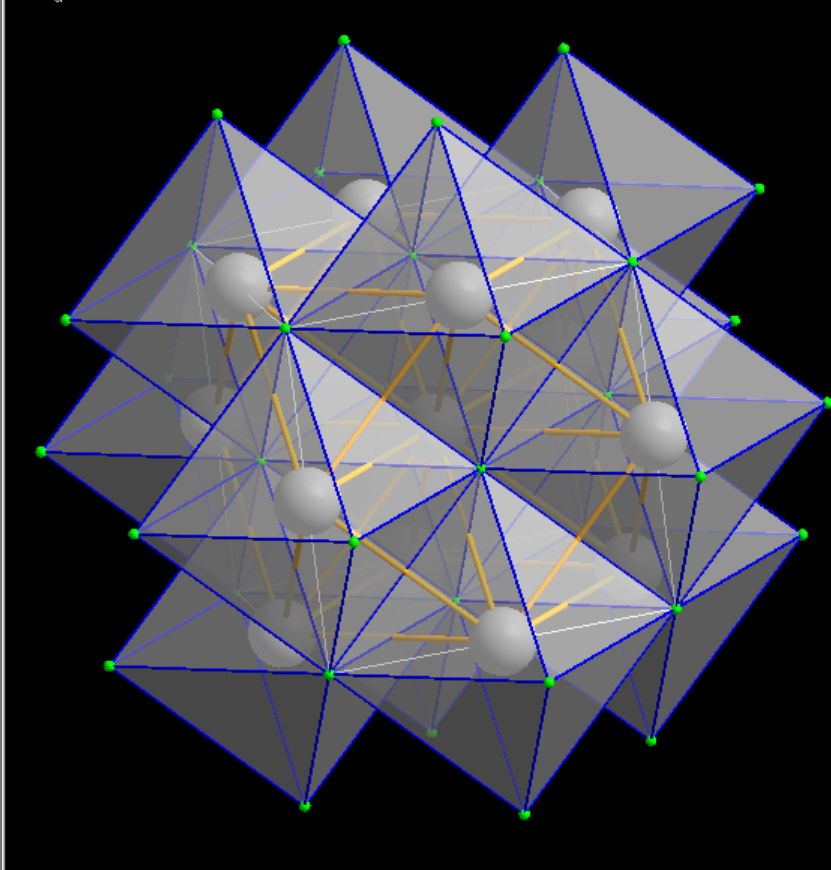
\includegraphics[width=0.28\textwidth]{assets/nacl/f.png}}
  \hfill
  \subcaptionbox{配位多面体设置}{%
    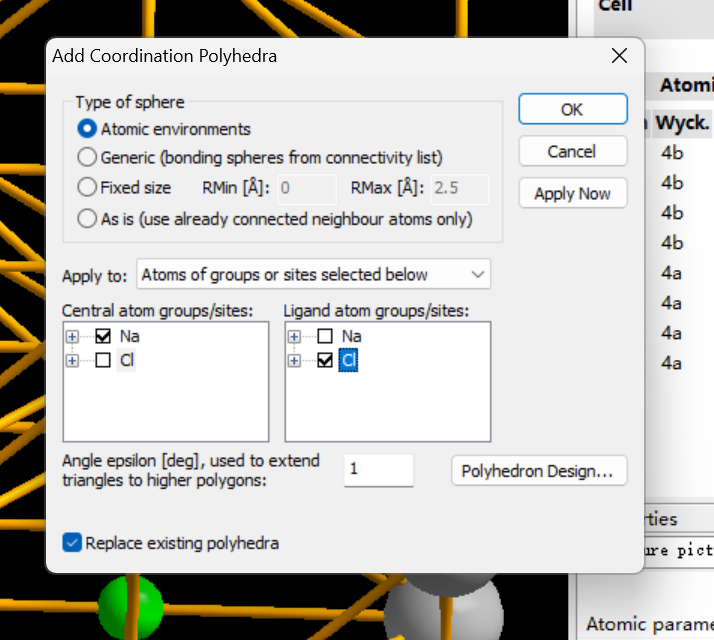
\includegraphics[width=0.24\textwidth]{assets/nacl/f1.png}}
  \caption{氯化钠（NaCl）结构的晶面与配位八面体}
  \label{fig:nacl-plane}
\end{figure}

\textbf{两套亚格子。}从图~\ref{fig:nacl-model} 可以看到 Na$^+$ 与 Cl$^-$ 沿晶胞棱方向
交替排列：Cl$^-$ 占顶点与面心，构成一套 FCC 点阵；Na$^+$ 占各棱中点与体心，相当于
另一套沿 $\langle100\rangle$ 平移 $a/2$ 的 FCC 点阵。两套亚格子叠加后，晶胞内有
4 个 Na$^+$ 与 4 个 Cl$^-$，即 4 个 NaCl 化学式单元。

两种离子的配位数都是 6，配位多面体为正八面体（图~\ref{fig:nacl-plane}(b)），Na--Cl
距离 $d=a/2=2.81$\,\AA。离子半径比 $r_+/r_-\approx0.54$ 落在八面体（六配位）的稳定
范围 $0.414\sim0.732$ 之内，与结构观察一致。再借助晶格常数计算理论密度：
\begin{equation}
  \rho=\frac{ZM}{N_Aa^3}
    =\frac{4\times58.44\ \mathrm{g/mol}}{6.022\times10^{23}\times
      (5.62\times10^{-8})^3\ \mathrm{cm^3}}
    \approx2.19\ \mathrm{g/cm^3}
\end{equation}
与实测密度（约 $2.16$ g/cm$^3$）接近，实际晶体中的缺陷使密度略低于理论值。KCl、LiF
等碱金属卤化物和 MgO、CaO、FeO 等氧化物都采取 NaCl 型结构。

% ==================== 2.3.2.5 金红石 ====================
\jiegou{2.3.2.5}{金红石结构（\texorpdfstring{TiO$_2$}{TiO2}）}

金红石型 TiO$_2$ 属四方晶系（$P\,4_2/m\,n\,m$，No.~136），建模输入值如表~\ref{tab:rutile}
所列。氧原子位于 $4f$ 位 $(x,x,0)$（$x\approx0.3$），表中列出的是模型中实际输入的
4 个等效氧原子坐标。

\begin{table}[H]
  \centering
  \caption{金红石（TiO$_2$）结构的建模参数}
  \label{tab:rutile}
  \begin{tabular}{ll}
    \toprule
    项目 & 参数 \\
    \midrule
    空间群 & $P\,4_2/m\,n\,m$（No.~136） \\
    晶格常数 & $a=b=4.6$\,\AA，$c=2.9634$\,\AA，$\alpha=\beta=\gamma=90^\circ$ \\
    原子坐标 & Ti：$(0,0,0)$、$(1/2,1/2,1/2)$（$2a$ 位）； \\
      & O：$(0.3,0.3,0)$、$(0.8,0.2,0.5)$； \\
      & O：$(0.7,0.7,0.5)$、$(0.2,0.8,0.5)$（$4f$ 位，$x\approx0.3$） \\
    化学式单元数 & $Z=2$ \\
    \bottomrule
  \end{tabular}
\end{table}

\begin{figure}[H]
  \centering
  \subcaptionbox{空间群与晶格常数设置}{%
    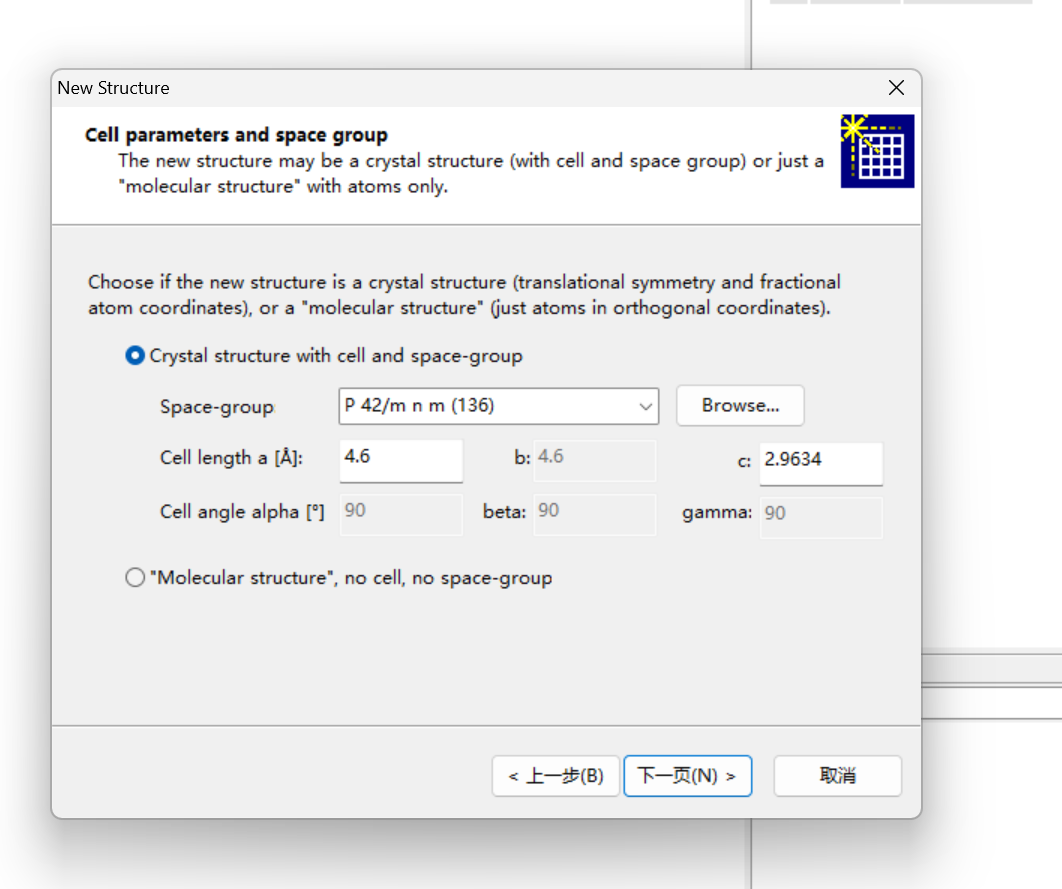
\includegraphics[width=0.44\textwidth]{assets/rutile/a.png}}
  \hfill
  \subcaptionbox{非对称单元原子（Ti、O）添加}{%
    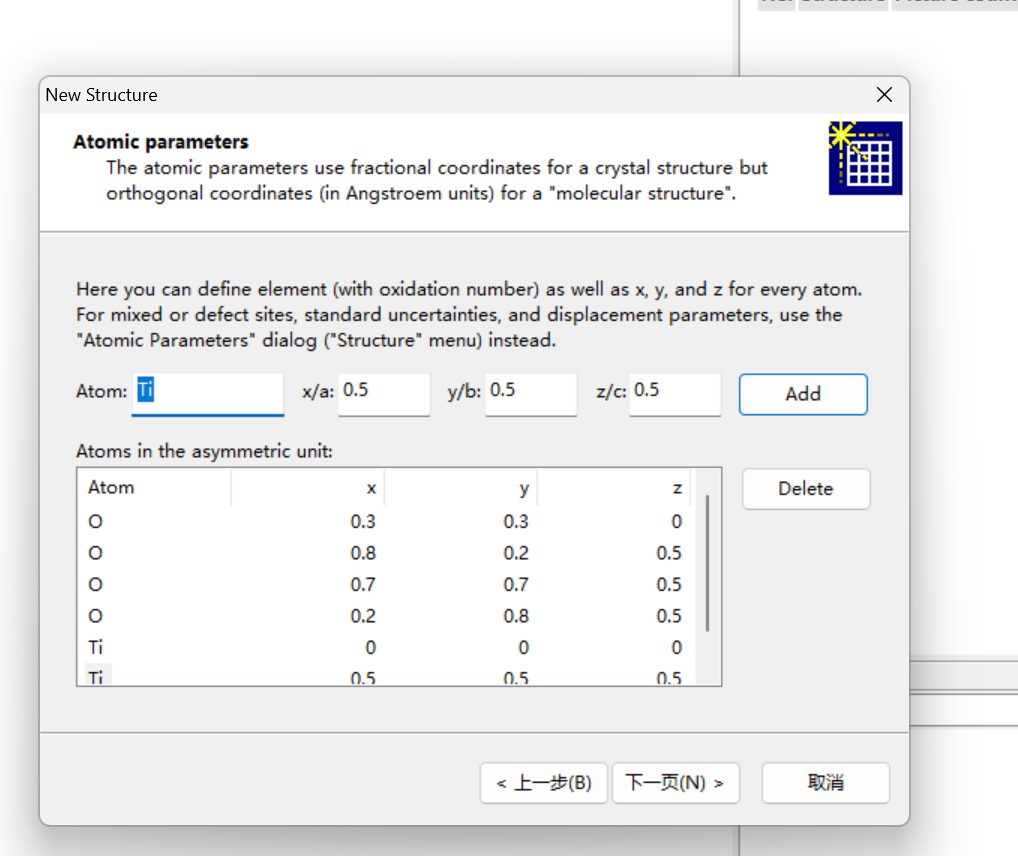
\includegraphics[width=0.44\textwidth]{assets/rutile/b.png}}
  \caption{金红石（TiO$_2$）结构的参数设置}
  \label{fig:rutile-param}
\end{figure}

\begin{figure}[H]
  \centering
  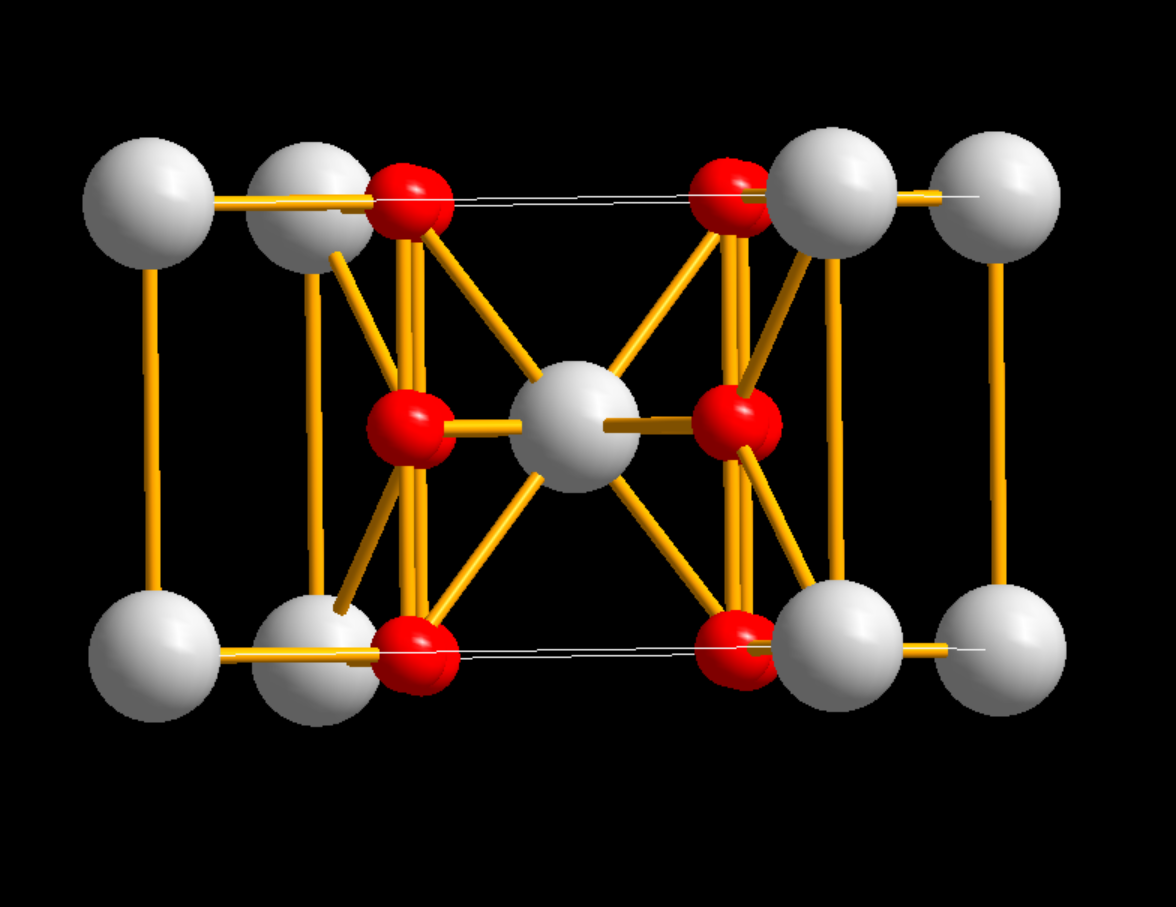
\includegraphics[width=0.5\textwidth]{assets/rutile/c.png}
  \caption{金红石（TiO$_2$）结构的晶体结构模型}
  \label{fig:rutile-model}
\end{figure}

\begin{figure}[H]
  \centering
  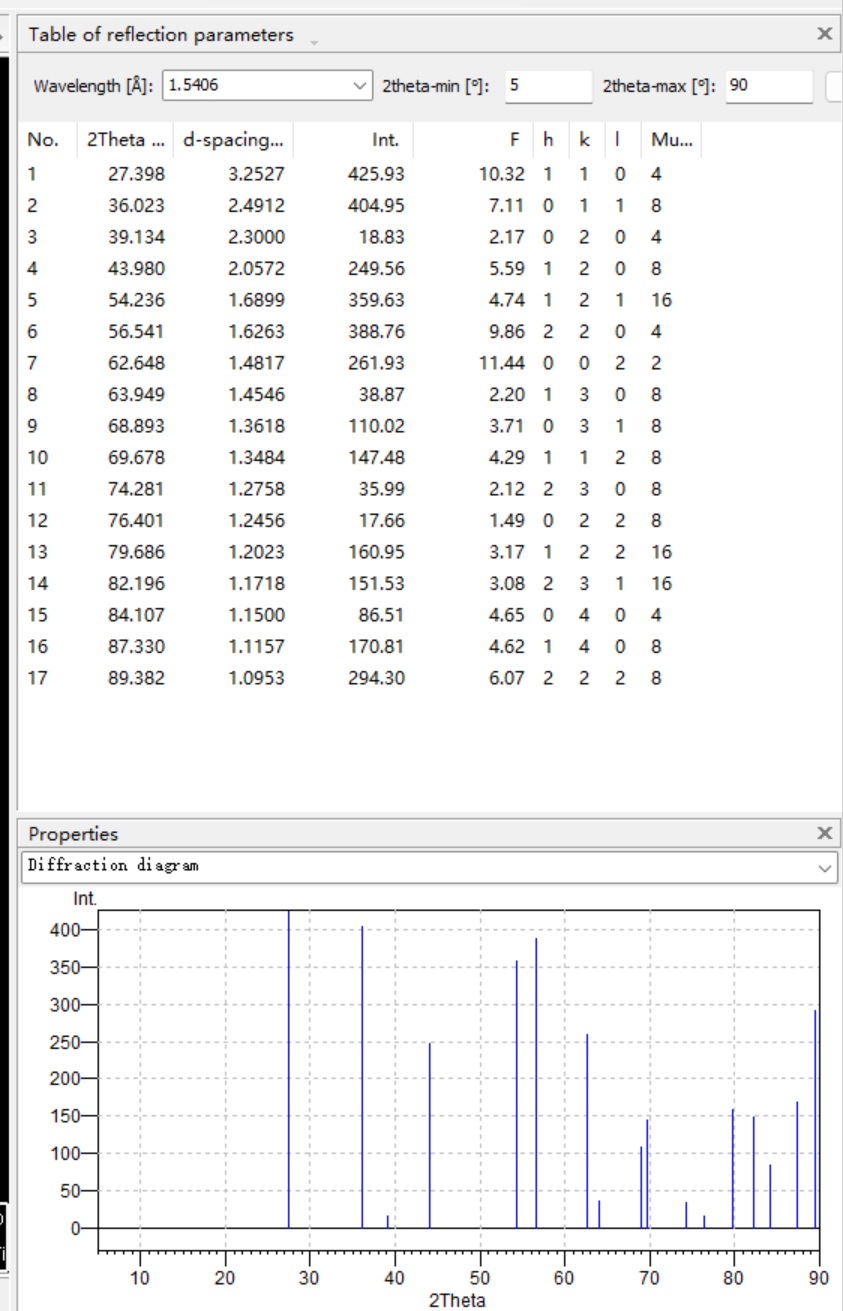
\includegraphics[width=0.4\textwidth]{assets/rutile/d.png}
  \caption{Diamond 模拟的金红石（TiO$_2$）结构粉末衍射图}
  \label{fig:rutile-xrd}
\end{figure}

\begin{figure}[H]
  \centering
  \subcaptionbox{晶面视图}{%
    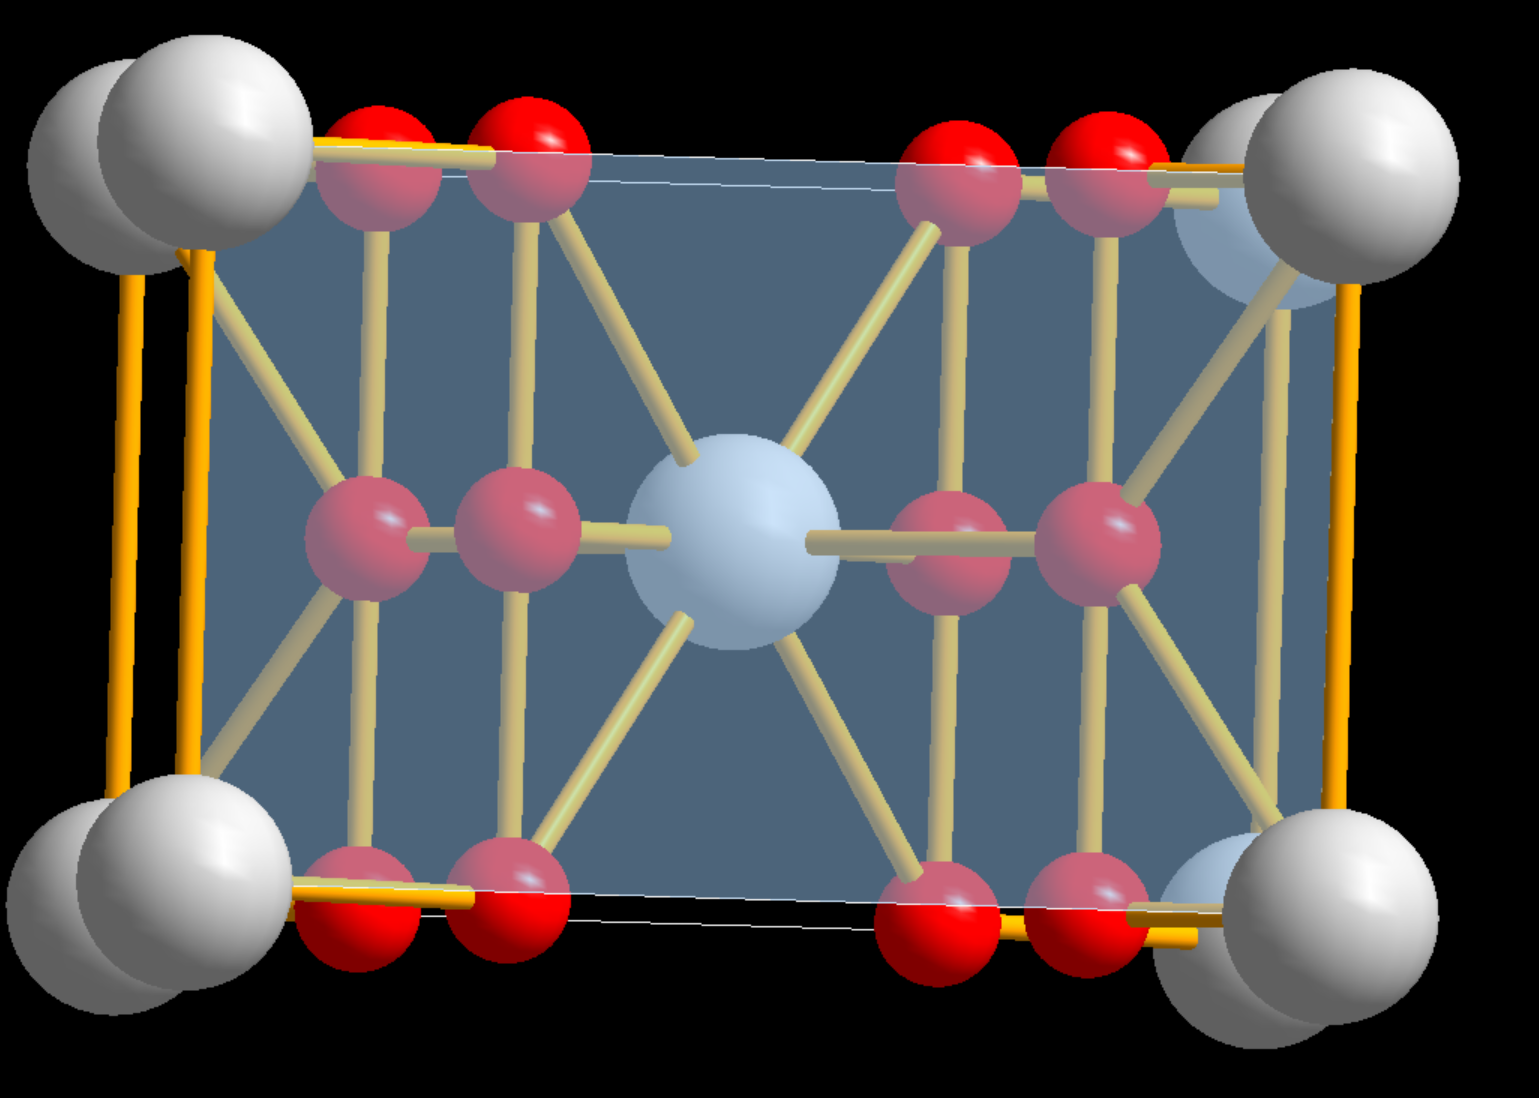
\includegraphics[width=0.44\textwidth]{assets/rutile/e.png}}
  \hfill
  \subcaptionbox{TiO$_6$ 配位八面体}{%
    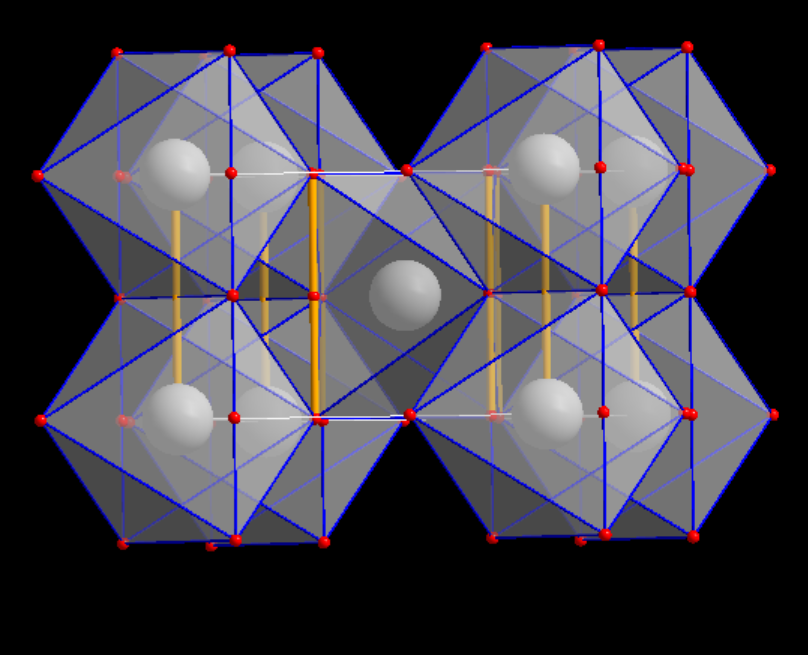
\includegraphics[width=0.28\textwidth]{assets/rutile/f.png}}
  \hfill
  \subcaptionbox{配位多面体设置}{%
    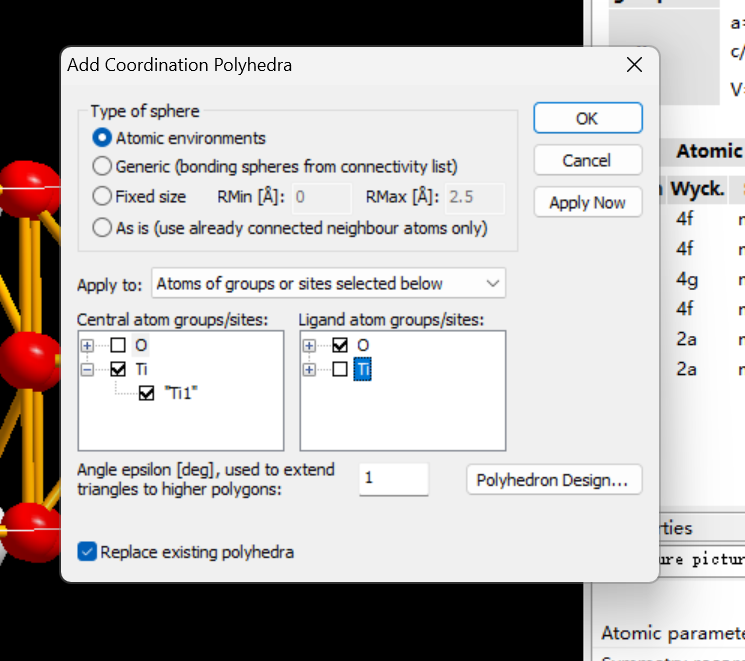
\includegraphics[width=0.24\textwidth]{assets/rutile/f1.png}}
  \caption{金红石（TiO$_2$）结构的晶面与配位八面体}
  \label{fig:rutile-plane}
\end{figure}

\textbf{结构特征。}每个 Ti$^{4+}$ 位于 TiO$_6$ 八面体中心，与 6 个 O$^{2-}$ 配位；
每个 O$^{2-}$ 反过来被 3 个 Ti$^{4+}$ 包围，呈平面三角配位。

把 $x=0.3$、$a=4.6$\,\AA、$c=2.9634$\,\AA 代入模型坐标，可以算出两类 Ti--O 键长：
赤道方向的 4 个键长为 $\sqrt{2}\,x\,a=\sqrt{2}\times0.3\times4.6\approx1.95$\,\AA；
顶点方向的 2 个键长为
\begin{equation}
  d_{\text{顶}}=\sqrt{2\bigl(\tfrac12-x\bigr)^2a^2+\frac{c^2}{4}}
    =\sqrt{2\times0.2^2\times4.6^2+2.9634^2/4}\approx1.97\ \text{\AA}
\end{equation}
八面体沿顶点方向被略微拉长。连接方式上，TiO$_6$ 八面体沿 $c$ 轴共棱连成无限链
（图~\ref{fig:rutile-plane}(b)），链与链之间再通过共用顶点（赤道氧）相连，构成三维
骨架；链内 Ti--Ti 距离因此较小，相邻链之间则靠共顶点氧联系。$P\,4_2/m\,n\,m$ 中
$4_2$ 螺旋轴沿 [001] 方向，$n$ 滑移面与镜面 $m$ 分别位于 [100]、[110] 方向，与
八面体链沿 $c$ 轴的螺旋排列相对应。

金红石相是常压下 TiO$_2$ 最稳定的晶型；SnO$_2$、MnO$_2$、GeO$_2$、RuO$_2$ 等也采取
金红石型结构。

% ==================== 2.3.2.6 锐钛矿 ====================
\jiegou{2.3.2.6}{锐钛矿结构（\texorpdfstring{TiO$_2$}{TiO2}）}

锐钛矿是 TiO$_2$ 的另一种常见晶型，属四方晶系，建模参数见表~\ref{tab:anatase}。
与金红石相比，锐钛矿晶胞为体心四方，$c$ 轴明显拉长。

\begin{table}[H]
  \centering
  \caption{锐钛矿（TiO$_2$）结构的建模参数}
  \label{tab:anatase}
  \begin{tabular}{ll}
    \toprule
    项目 & 参数 \\
    \midrule
    空间群 & $I\,4_1/a\,m\,d$（No.~141） \\
    晶格常数 & $a=b=3.784$\,\AA，$c=9.5146$\,\AA，$\alpha=\beta=\gamma=90^\circ$ \\
    原子坐标 & Ti：$(0,0,0)$（$4a$ 位）；O：$(0,0,0.208)$（$8e$ 位） \\
    化学式单元数 & $Z=4$ \\
    \bottomrule
  \end{tabular}
\end{table}

\begin{figure}[H]
  \centering
  \subcaptionbox{空间群与晶格常数设置}{%
    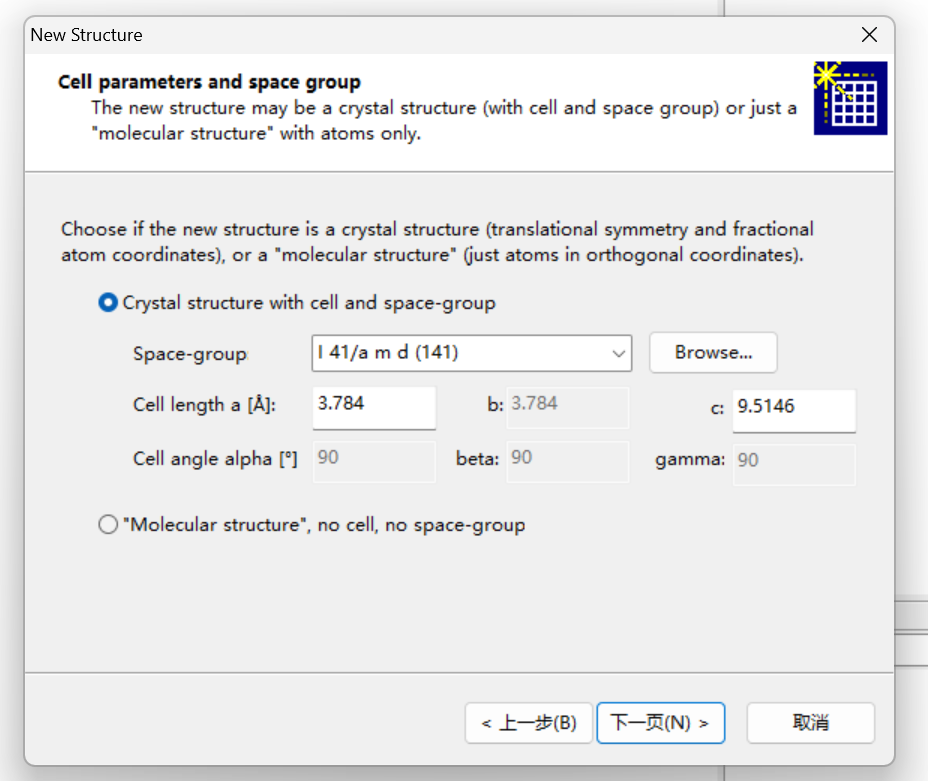
\includegraphics[width=0.44\textwidth]{assets/anatase/a.png}}
  \hfill
  \subcaptionbox{非对称单元原子（Ti、O）添加}{%
    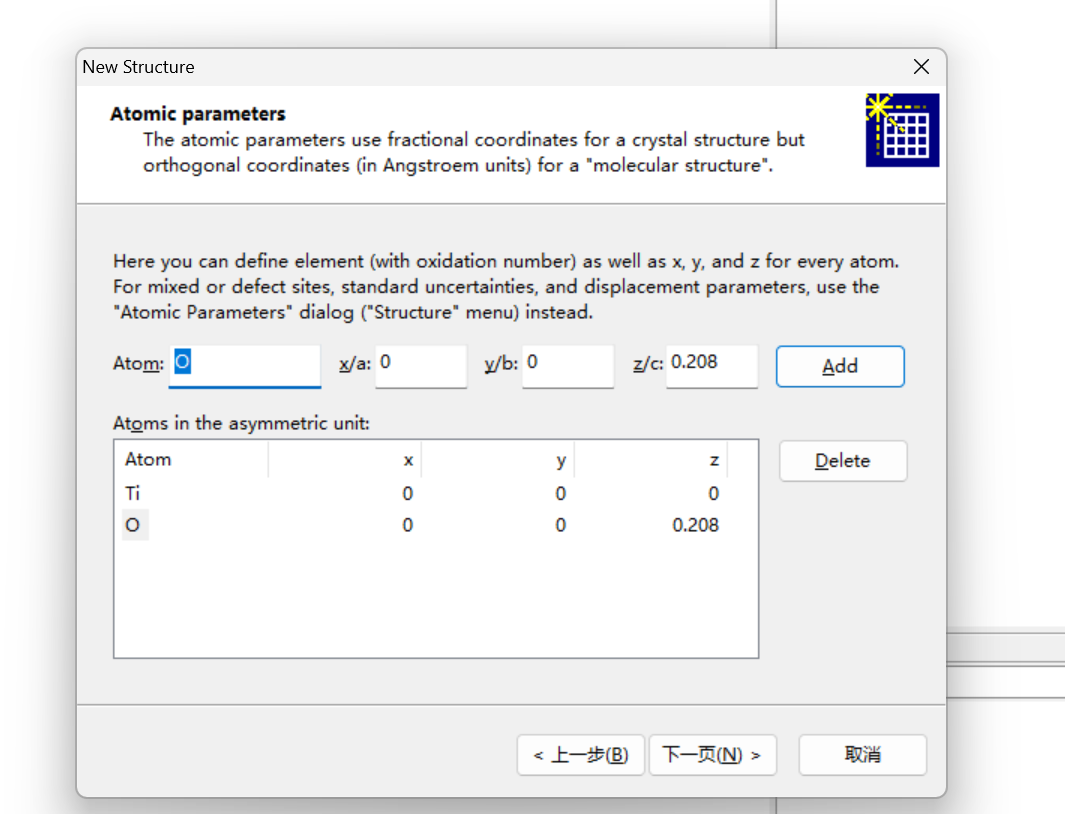
\includegraphics[width=0.44\textwidth]{assets/anatase/b.png}}
  \caption{锐钛矿（TiO$_2$）结构的参数设置}
  \label{fig:anatase-param}
\end{figure}

\begin{figure}[H]
  \centering
  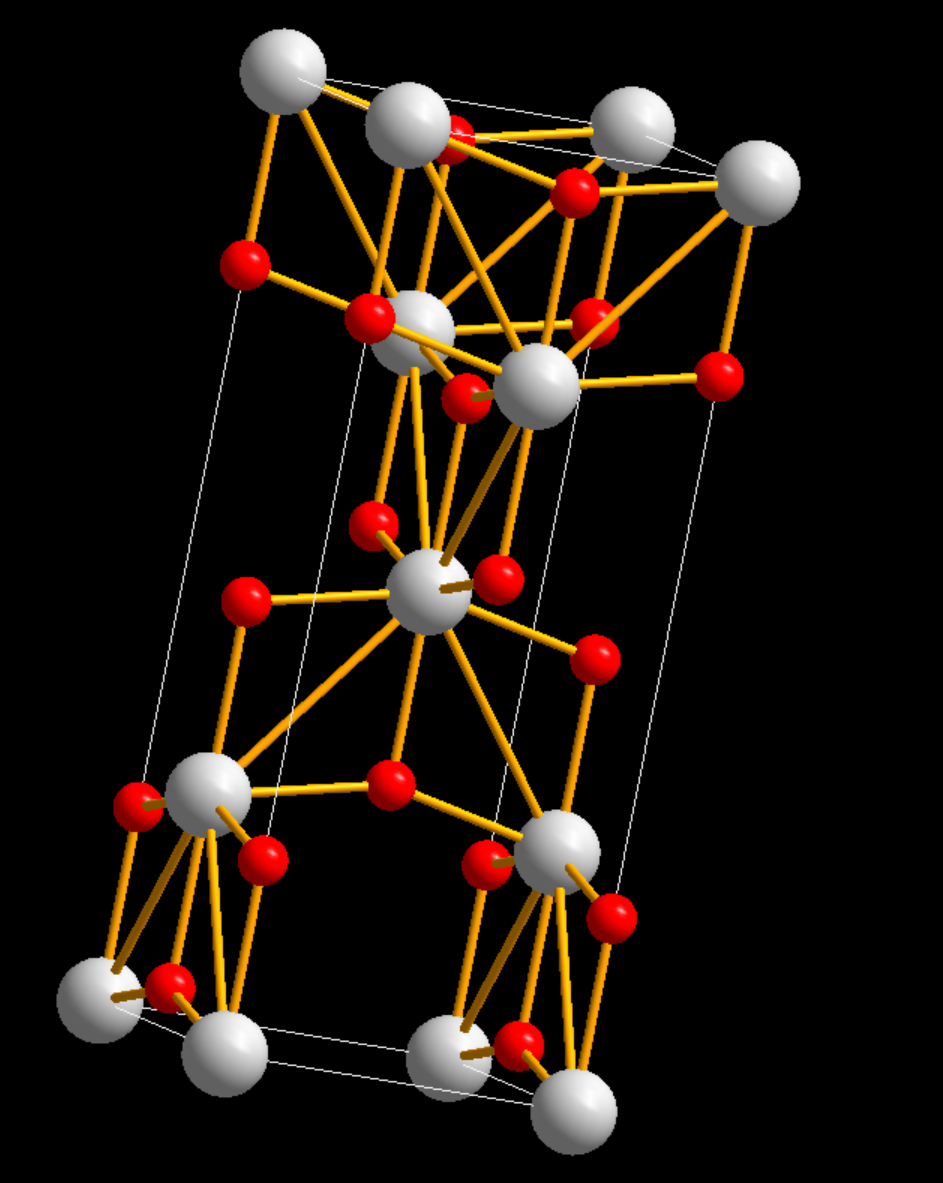
\includegraphics[width=0.5\textwidth]{assets/anatase/c.png}
  \caption{锐钛矿（TiO$_2$）结构的晶体结构模型}
  \label{fig:anatase-model}
\end{figure}

\begin{figure}[H]
  \centering
  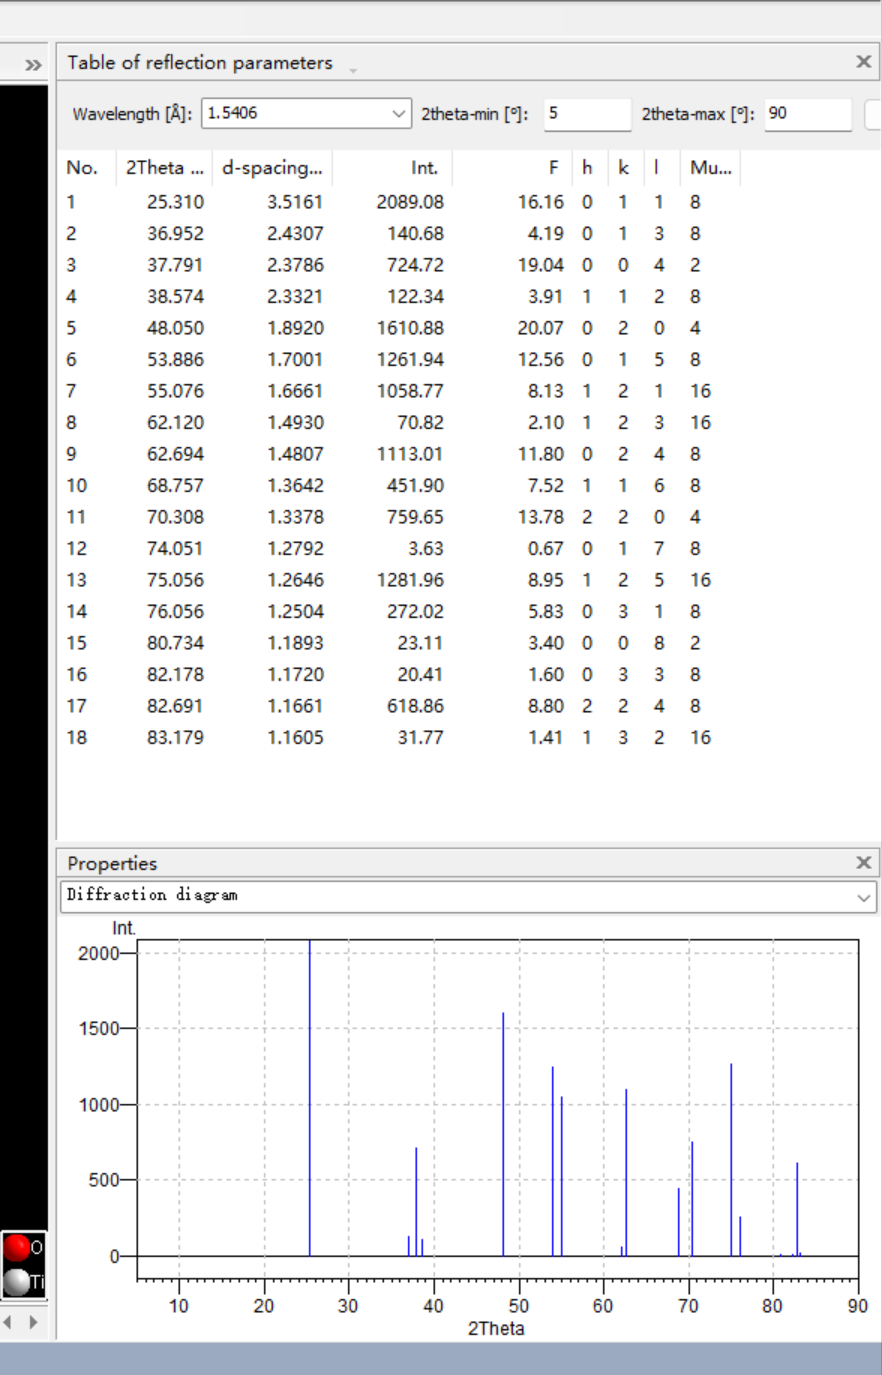
\includegraphics[width=0.4\textwidth]{assets/anatase/d.png}
  \caption{Diamond 模拟的锐钛矿（TiO$_2$）结构粉末衍射图}
  \label{fig:anatase-xrd}
\end{figure}

\begin{figure}[H]
  \centering
  \subcaptionbox{晶面视图}{%
    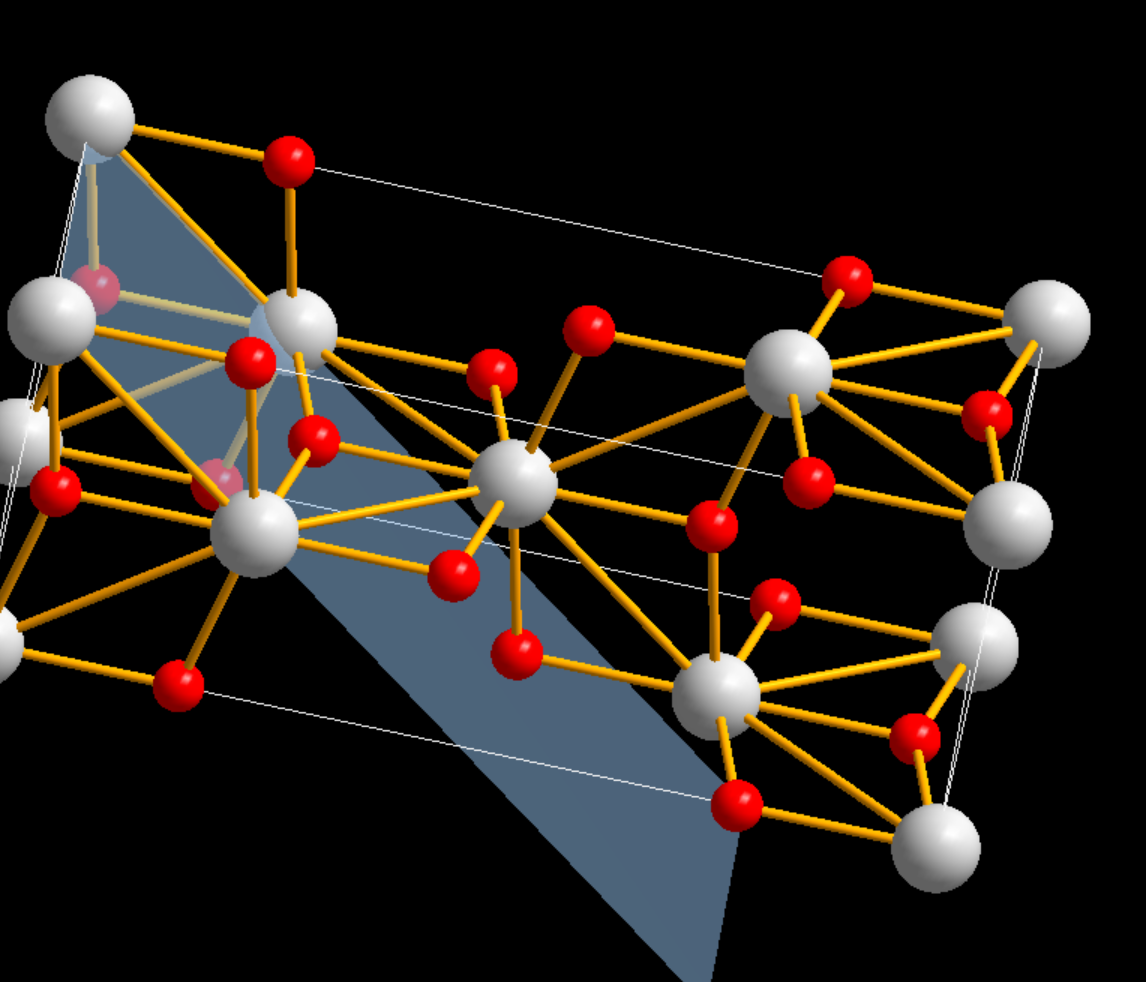
\includegraphics[width=0.44\textwidth]{assets/anatase/e.png}}
  \hfill
  \subcaptionbox{TiO$_6$ 配位八面体}{%
    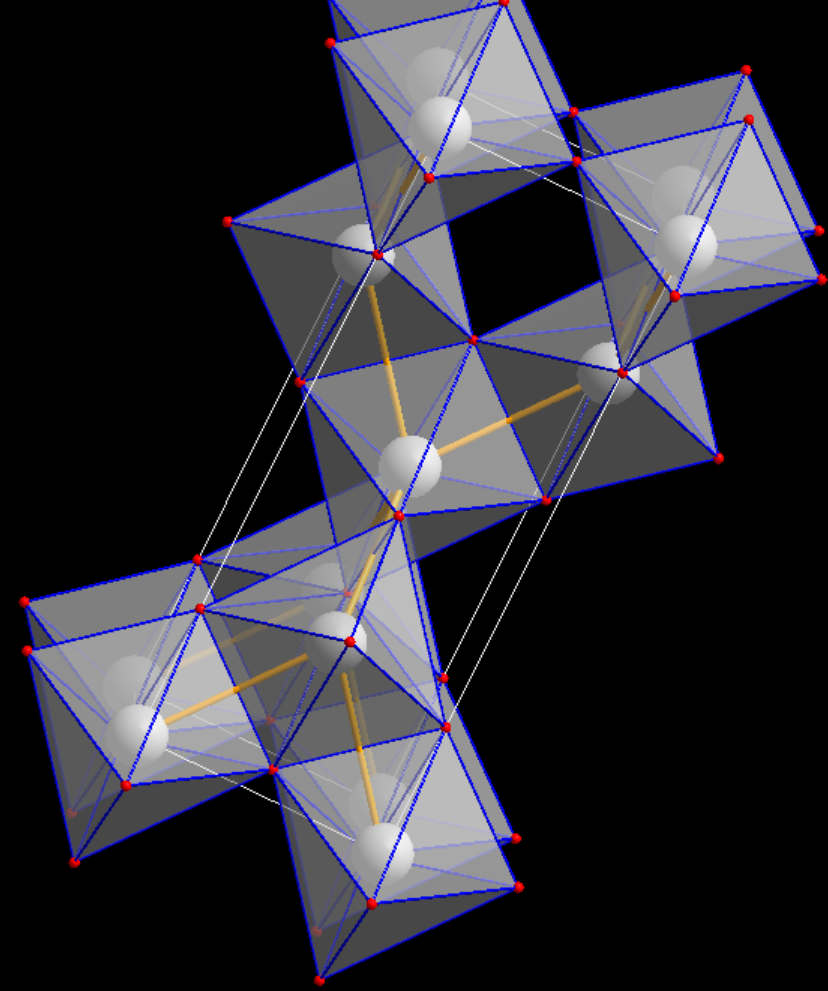
\includegraphics[width=0.28\textwidth]{assets/anatase/f.png}}
  \hfill
  \subcaptionbox{配位多面体设置}{%
    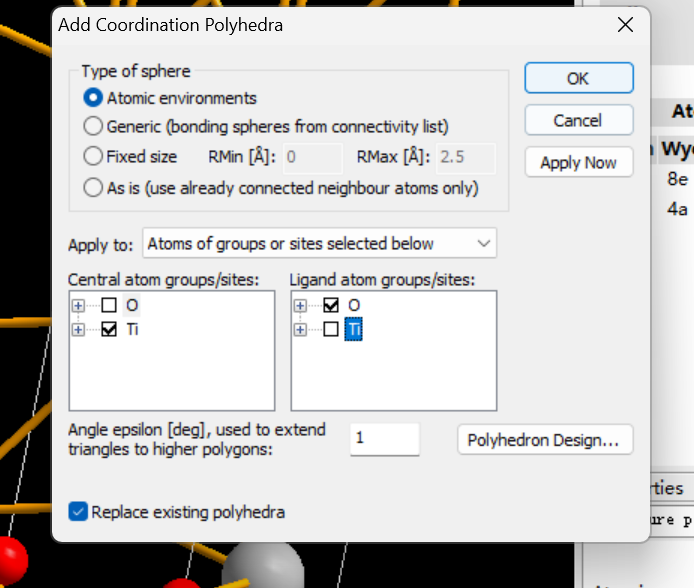
\includegraphics[width=0.24\textwidth]{assets/anatase/f1.png}}
  \caption{锐钛矿（TiO$_2$）结构的晶面与配位八面体}
  \label{fig:anatase-plane}
\end{figure}

\textbf{结构特征。}锐钛矿中 Ti$^{4+}$ 同样位于 TiO$_6$ 八面体中心，但八面体的连接
方式与金红石不同。

\begin{enumerate}[label=（\arabic*）]
  \item \textbf{TiO$_6$ 八面体}：由模型参数计算，沿 $c$ 轴方向的 2 个顶点 Ti--O 键长为
    $0.208\,c\approx1.98$\,\AA，赤道方向的 4 个 Ti--O 键长约为 $1.93$\,\AA
    （$=\sqrt{(a/2)^2+[(1/4-0.208)c]^2}$），八面体略有畸变。每个 O$^{2-}$ 与 3 个
    Ti$^{4+}$ 配位，其中 1 个键略长、2 个略短。
  \item \textbf{八面体的连接方式}：TiO$_6$ 八面体之间全部通过共边连接，形成沿
    $\langle100\rangle$、$\langle010\rangle$ 方向延伸的锯齿状链（图~\ref{fig:anatase-plane}(b)）。
    与金红石（共棱成链、链间共角）相比，锐钛矿的骨架更加开放，密度更低，晶胞中空位
    更大，这是锐钛矿 TiO$_2$ 在光催化等领域表现出特殊活性的结构原因之一。
  \item \textbf{空间群}：$I\,4_1/a\,m\,d$ 中 $I$ 为体心点阵，$4_1$ 螺旋轴沿 [001]，
    $a$ 滑移面、镜面 $m$ 与 $d$ 金刚石滑移面位于相应的特征方向。
\end{enumerate}

金红石与锐钛矿是 TiO$_2$ 最常见的两种晶型，二者的共同点是 TiO$_6$ 八面体配位，区别
在于八面体的连接方式，体现出``配位多面体—连接方式—晶体结构''的描述思路。

% ==================== 2.3.2.7 萤石 ====================
\jiegou{2.3.2.7}{萤石结构（\texorpdfstring{CaF$_2$}{CaF2}）}

以 CaF$_2$ 为例建立模型，建模参数见表~\ref{tab:fluorite}。萤石结构中 Ca$^{2+}$ 占据
面心立方位置，F$^-$ 占据晶胞内全部 8 个四面体间隙。

\begin{table}[H]
  \centering
  \caption{萤石（CaF$_2$）结构的建模参数}
  \label{tab:fluorite}
  \begin{tabular}{ll}
    \toprule
    项目 & 参数 \\
    \midrule
    空间群 & $F\,m\,\bar3\,m$（No.~225） \\
    晶格常数 & $a=b=c=5.462$\,\AA，$\alpha=\beta=\gamma=90^\circ$ \\
    原子坐标 & Ca：$(0,0,0)$（$4a$ 位）；F：$(1/4,1/4,1/4)$（$8c$ 位） \\
    化学式单元数 & $Z=4$ \\
    \bottomrule
  \end{tabular}
\end{table}

\begin{figure}[H]
  \centering
  \subcaptionbox{空间群与晶格常数设置}{%
    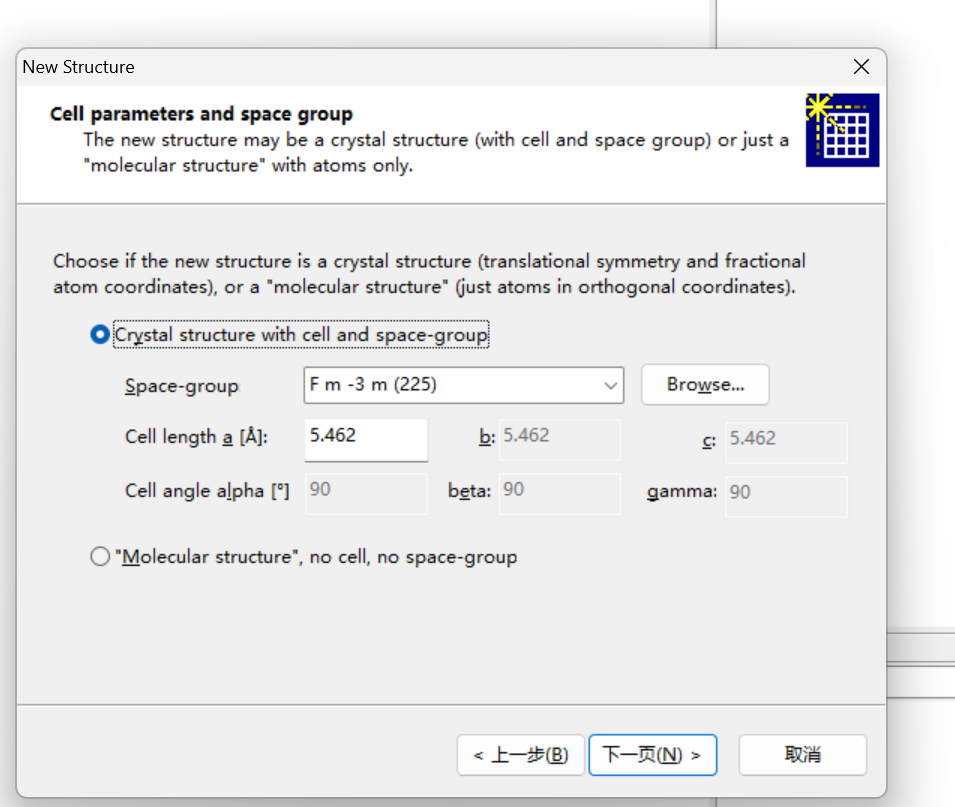
\includegraphics[width=0.44\textwidth]{assets/fluorite/a.png}}
  \hfill
  \subcaptionbox{非对称单元原子（Ca、F）添加}{%
    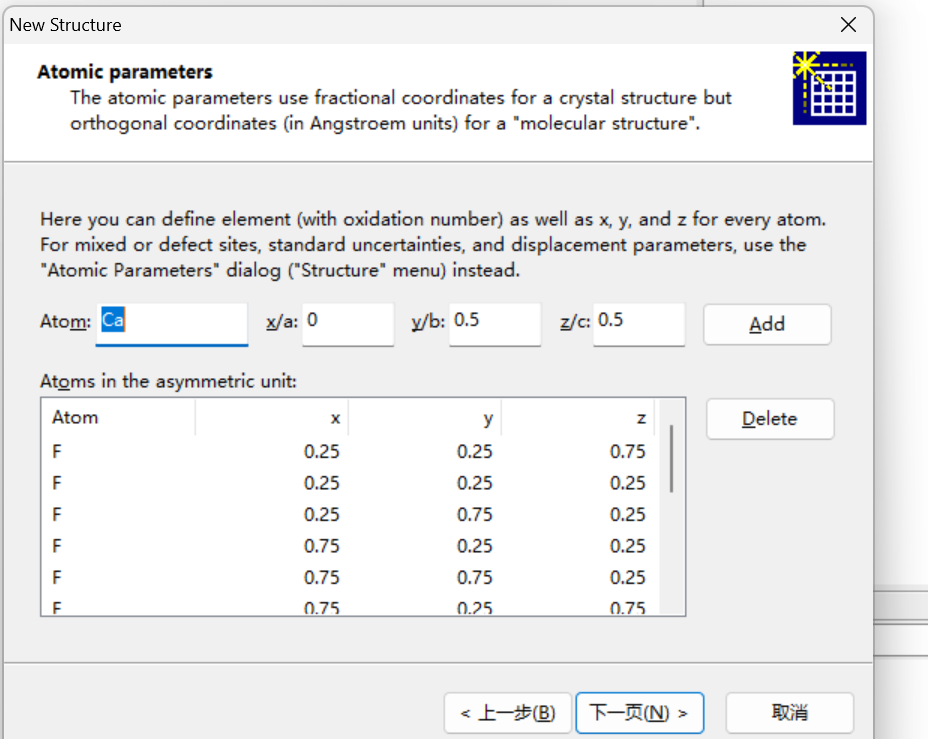
\includegraphics[width=0.44\textwidth]{assets/fluorite/b.png}}
  \caption{萤石（CaF$_2$）结构的参数设置}
  \label{fig:fluorite-param}
\end{figure}

\begin{figure}[H]
  \centering
  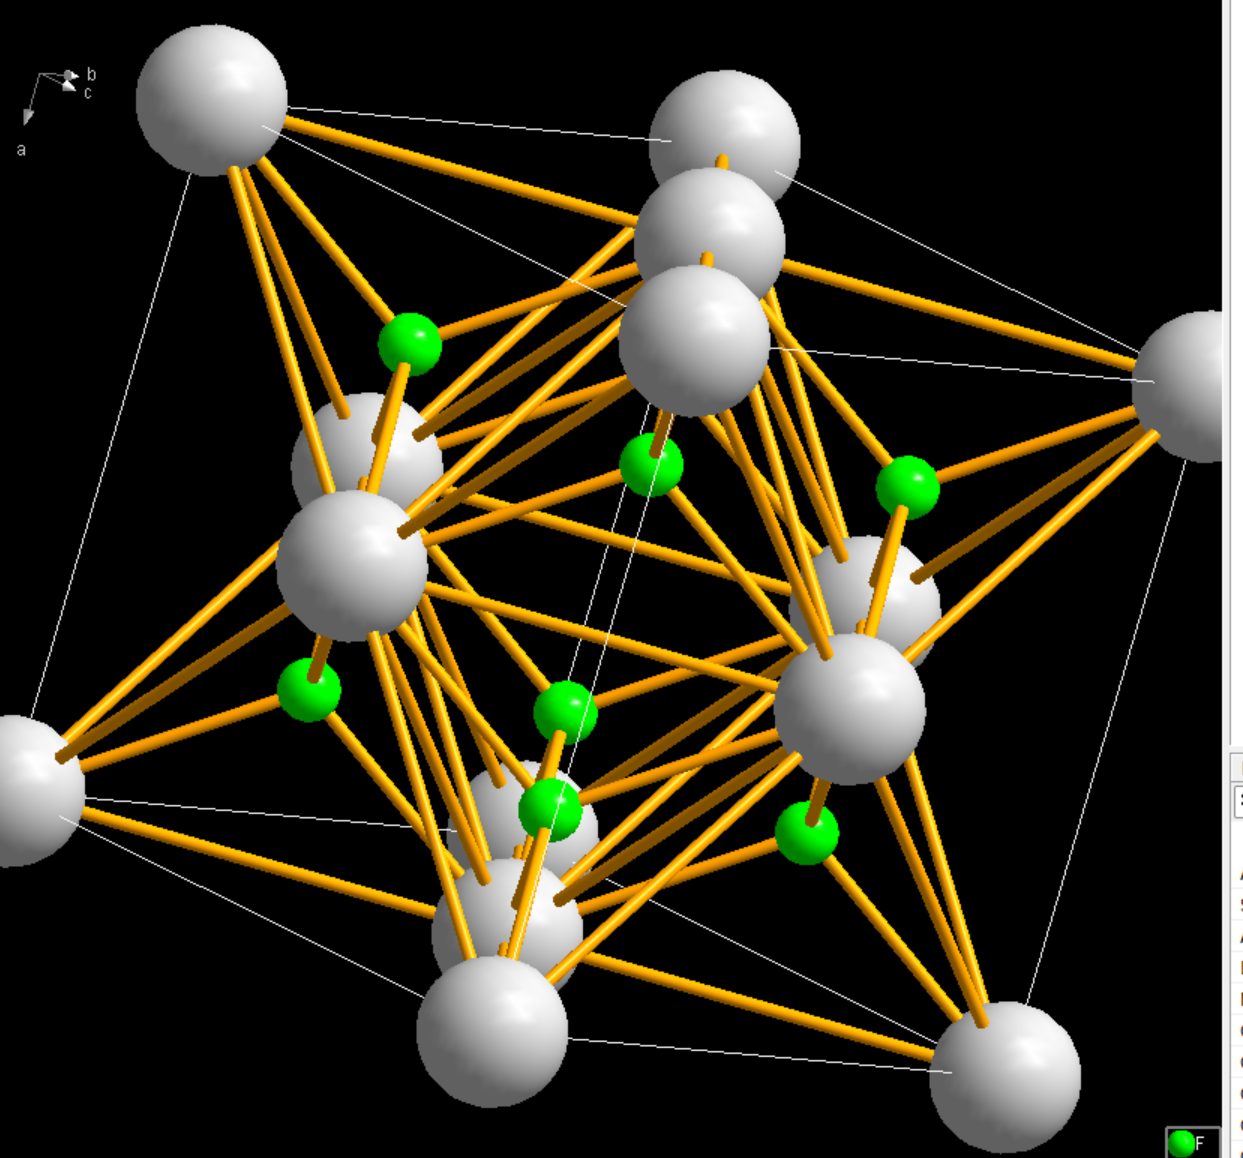
\includegraphics[width=0.5\textwidth]{assets/fluorite/c.png}
  \caption{萤石（CaF$_2$）结构的晶体结构模型}
  \label{fig:fluorite-model}
\end{figure}

\begin{figure}[H]
  \centering
  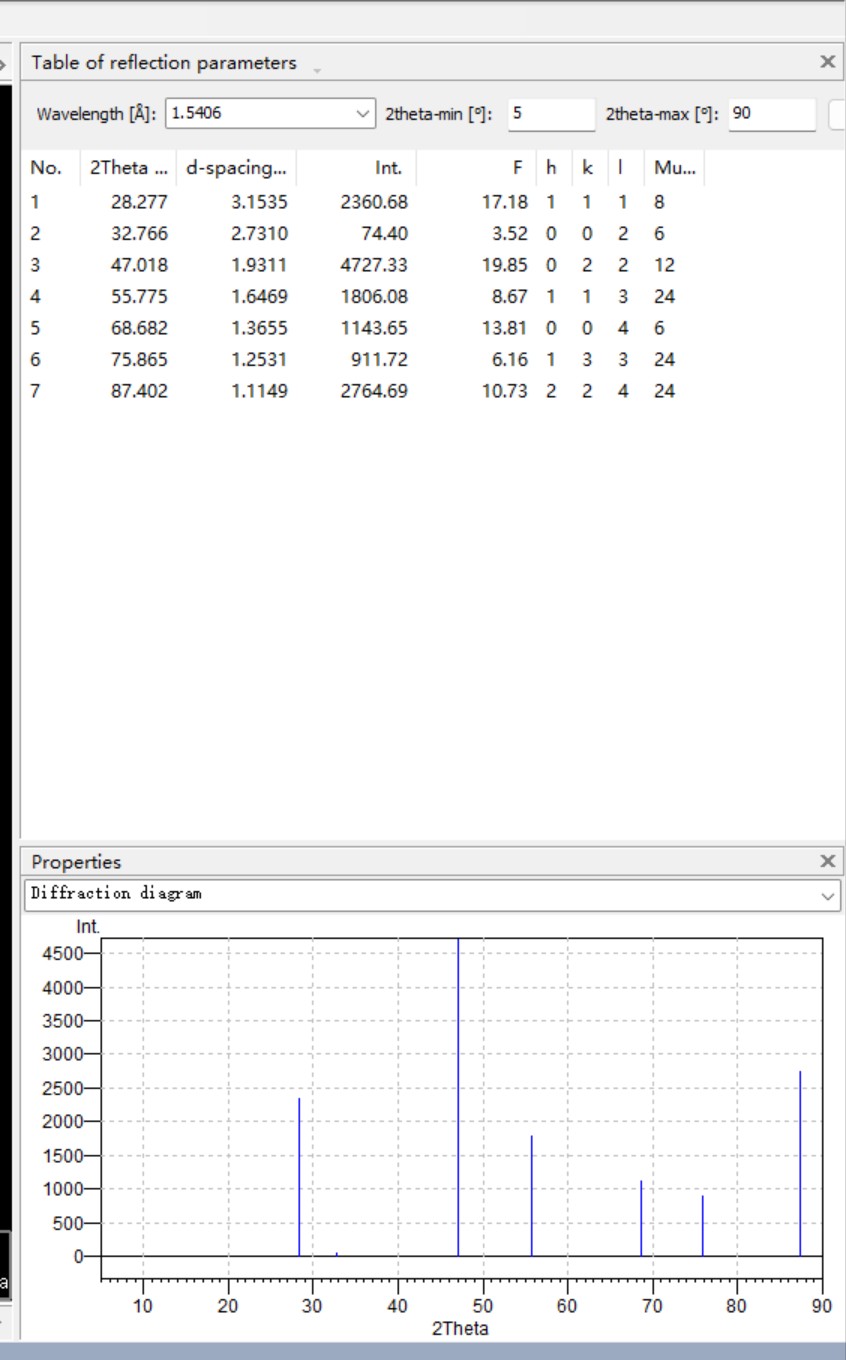
\includegraphics[width=0.4\textwidth]{assets/fluorite/d.png}
  \caption{Diamond 模拟的萤石（CaF$_2$）结构粉末衍射图}
  \label{fig:fluorite-xrd}
\end{figure}

\begin{figure}[H]
  \centering
  \subcaptionbox{晶面视图}{%
    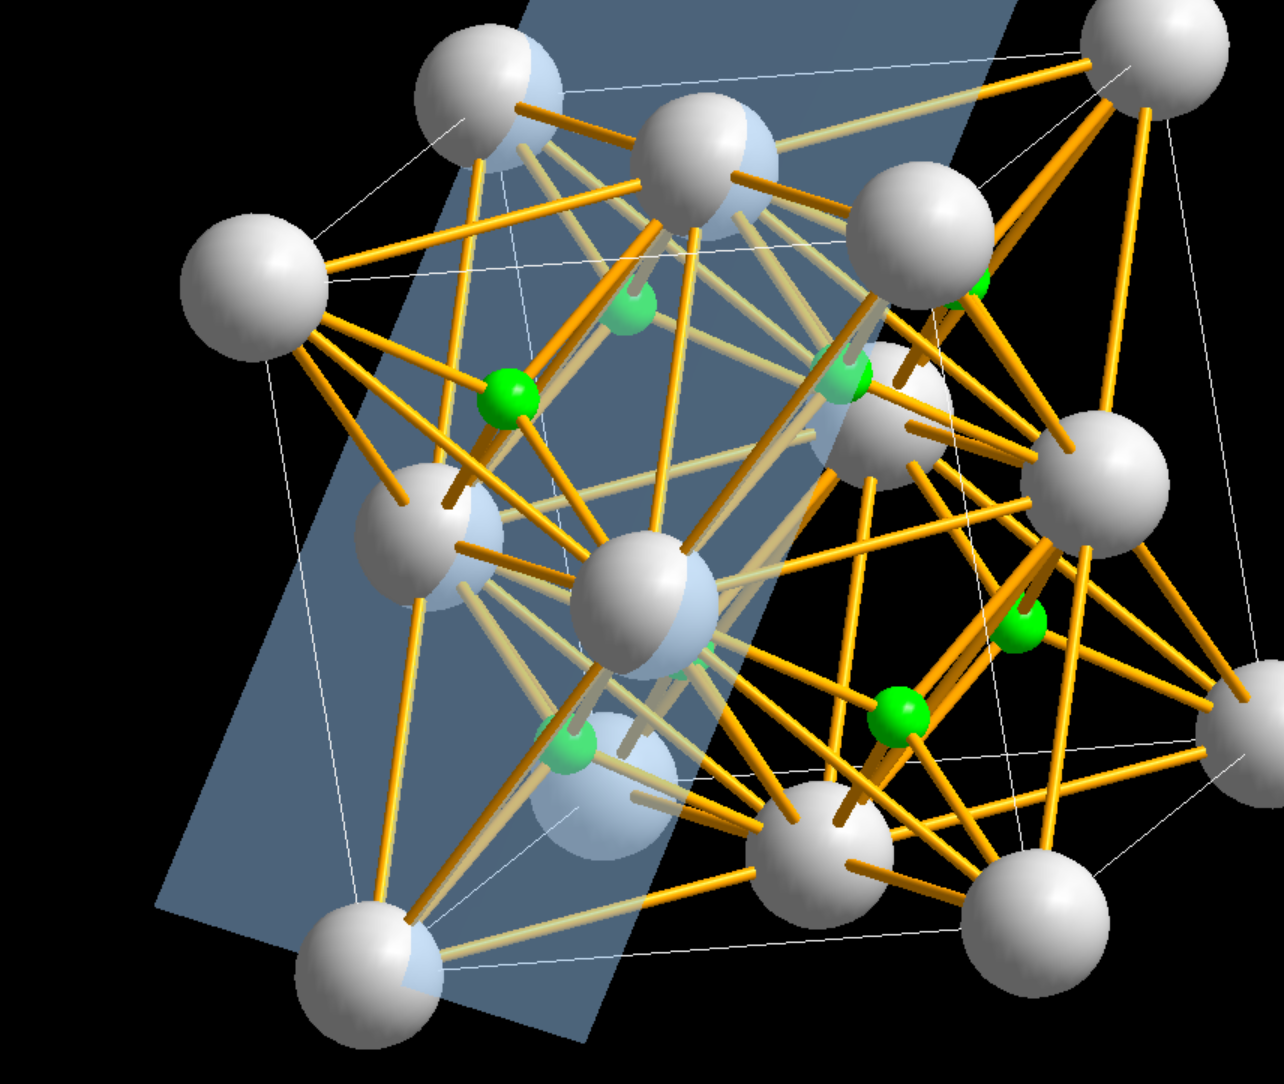
\includegraphics[width=0.44\textwidth]{assets/fluorite/e.png}}
  \hfill
  \subcaptionbox{Ca 的立方配位与 F 的四面体配位}{%
    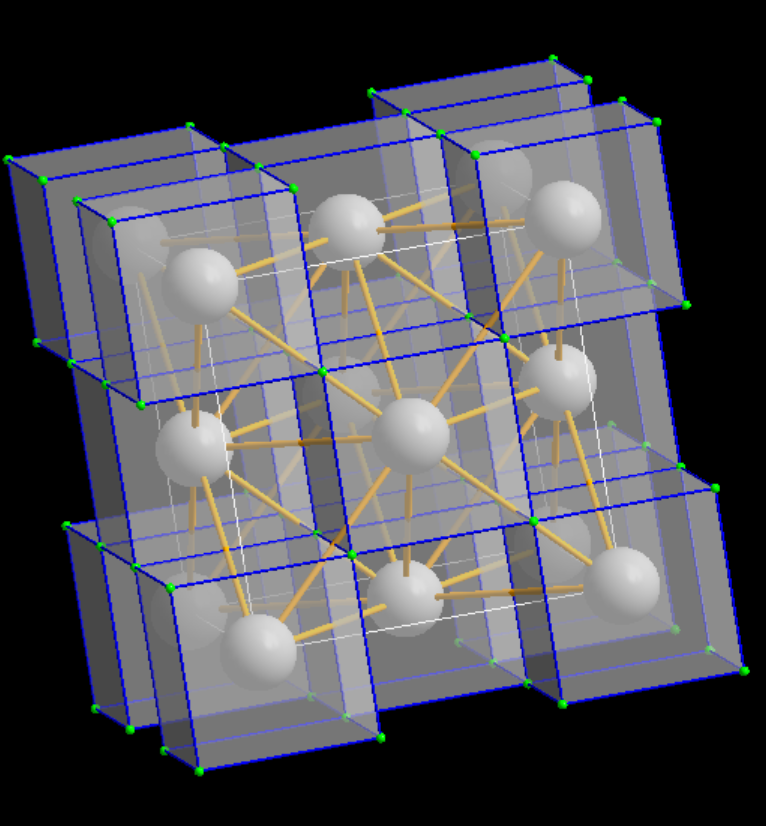
\includegraphics[width=0.28\textwidth]{assets/fluorite/f.png}}
  \hfill
  \subcaptionbox{配位多面体设置}{%
    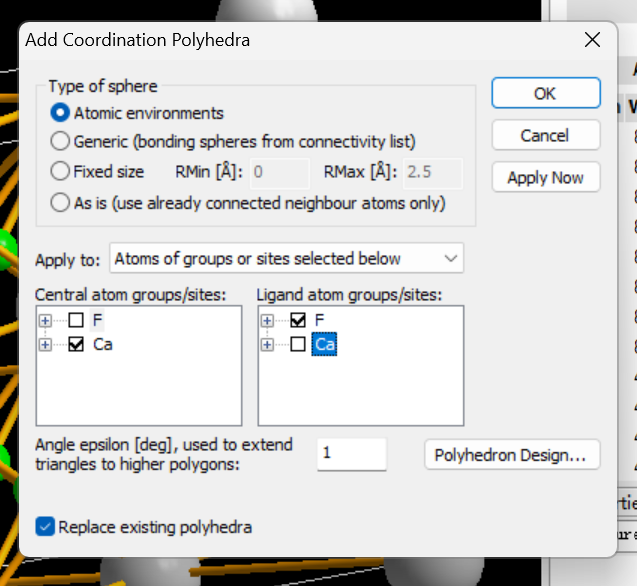
\includegraphics[width=0.24\textwidth]{assets/fluorite/f1.png}}
  \caption{萤石（CaF$_2$）结构的晶面与配位多面体}
  \label{fig:fluorite-plane}
\end{figure}

\textbf{结构特征。}萤石结构可用两种视角描述：Ca$^{2+}$ 构成面心立方骨架，F$^-$ 填充
其中全部 8 个四面体间隙；或视为 F$^-$ 构成简单立方骨架，Ca$^{2+}$ 间隔填充其中一半
立方体空隙。

\begin{enumerate}[label=（\arabic*）]
  \item \textbf{配位数}：Ca$^{2+}$ 被 8 个 F$^-$ 包围，配位多面体为立方体
    （图~\ref{fig:fluorite-plane}(b)）；F$^-$ 被 4 个 Ca$^{2+}$ 包围，配位多面体为
    四面体。键长 $d=\sqrt{3}a/4=\sqrt{3}\times5.462/4\approx2.37$\,\AA。
  \item \textbf{间隙填充}：面心立方点阵的四面体间隙（如 $(1/4,1/4,1/4)$ 及其对称
    等效位置）共有 8 个，在萤石结构中被 F$^-$ 全部占据，而八面体间隙
    $(1/2,1/2,1/2)$ 保持空缺。这种``部分填充''特点使萤石结构具有较高的离子迁移空间，
    ZrO$_2$、CeO$_2$ 等萤石型氧化物是重要的快离子导体与燃料电池电解质材料。
  \item \textbf{反萤石结构}：若阴阳离子互换（碱金属占据 F$^-$ 位、O$^{2-}$ 占据
    Ca$^{2+}$ 位），即得反萤石结构，如 Na$_2$O、Li$_2$O。
\end{enumerate}

具有萤石型结构的典型物质包括 CaF$_2$、BaF$_2$、UO$_2$、ThO$_2$ 及高温相 ZrO$_2$ 等。

% ==================== 2.3.2.8 金刚石 ====================
\jiegou{2.3.2.8}{金刚石结构}

金刚石结构可视为两套面心立方点阵沿体对角线平移 $(1/4,1/4,1/4)$ 相互穿插而成。这里
用硅演示（$a=5.42$\,\AA 为 Si 的特征值），它与金刚石碳同属金刚石型结构；参数见
表~\ref{tab:diamond}。

\begin{table}[H]
  \centering
  \caption{金刚石结构的建模参数（以 Si 为例）}
  \label{tab:diamond}
  \begin{tabular}{ll}
    \toprule
    项目 & 参数 \\
    \midrule
    空间群 & $F\,d\,\bar3\,m$（No.~227） \\
    晶格常数 & $a=b=c=5.42$\,\AA，$\alpha=\beta=\gamma=90^\circ$ \\
    原子坐标 & Si：$(0,0,0)$（$8a$ 位，另含 $(1/4,1/4,1/4)$ 平移的等效位） \\
    化学式单元数 & $Z=8$ \\
    \bottomrule
  \end{tabular}
\end{table}

\begin{figure}[H]
  \centering
  \subcaptionbox{空间群与晶格常数设置}{%
    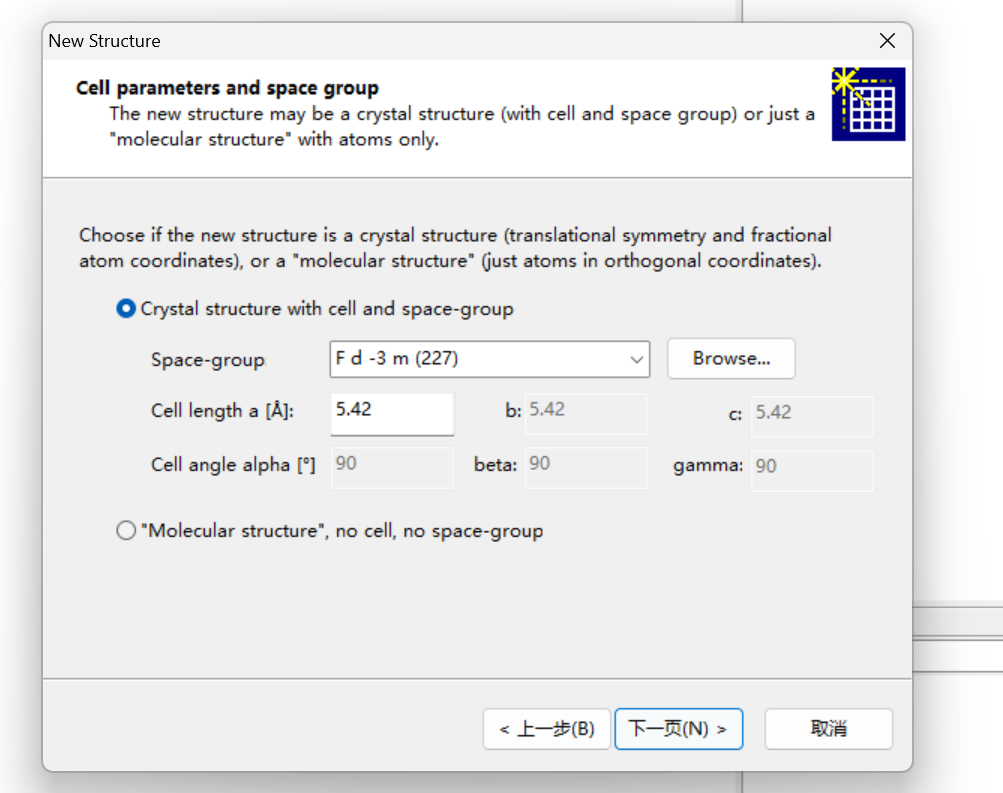
\includegraphics[width=0.44\textwidth]{assets/diamond/a.png}}
  \hfill
  \subcaptionbox{非对称单元原子（Si）添加}{%
    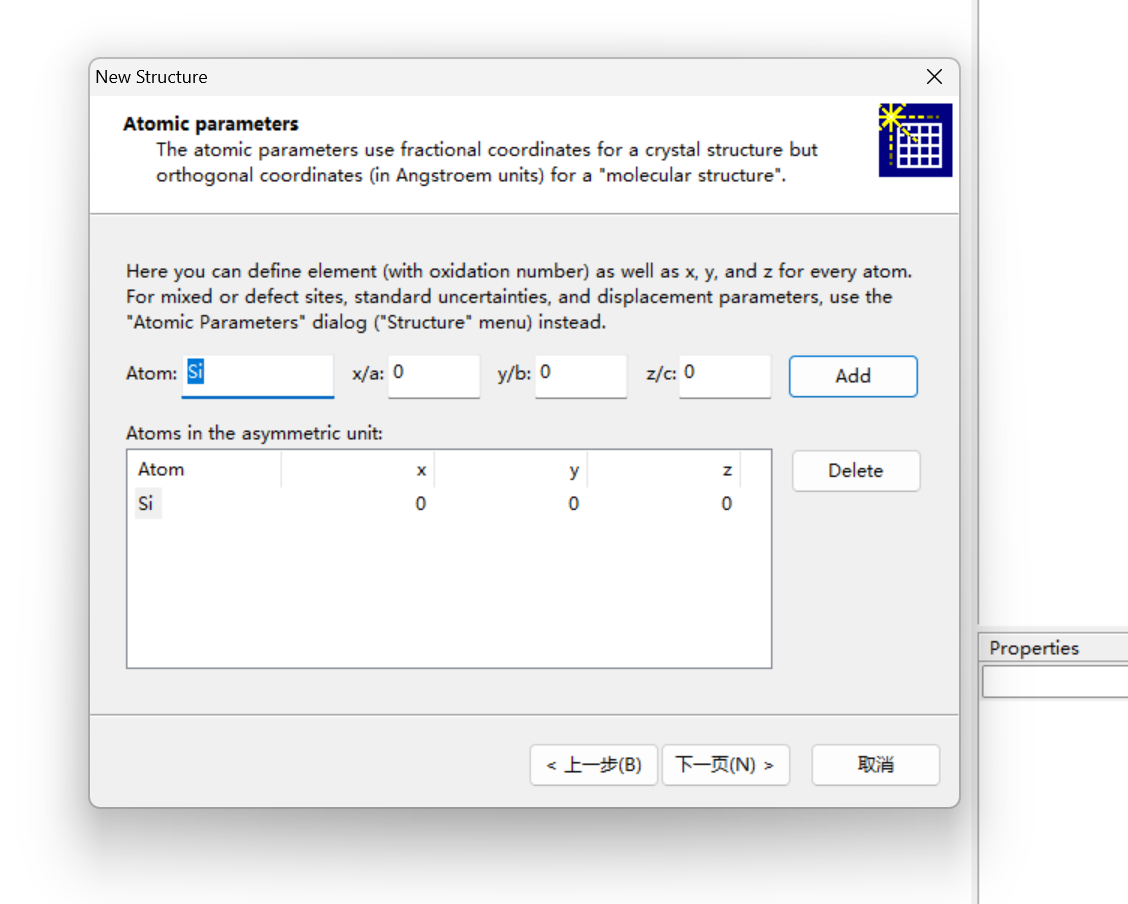
\includegraphics[width=0.44\textwidth]{assets/diamond/b.png}}
  \caption{金刚石结构的参数设置（以 Si 为例）}
  \label{fig:diamond-param}
\end{figure}

\begin{figure}[H]
  \centering
  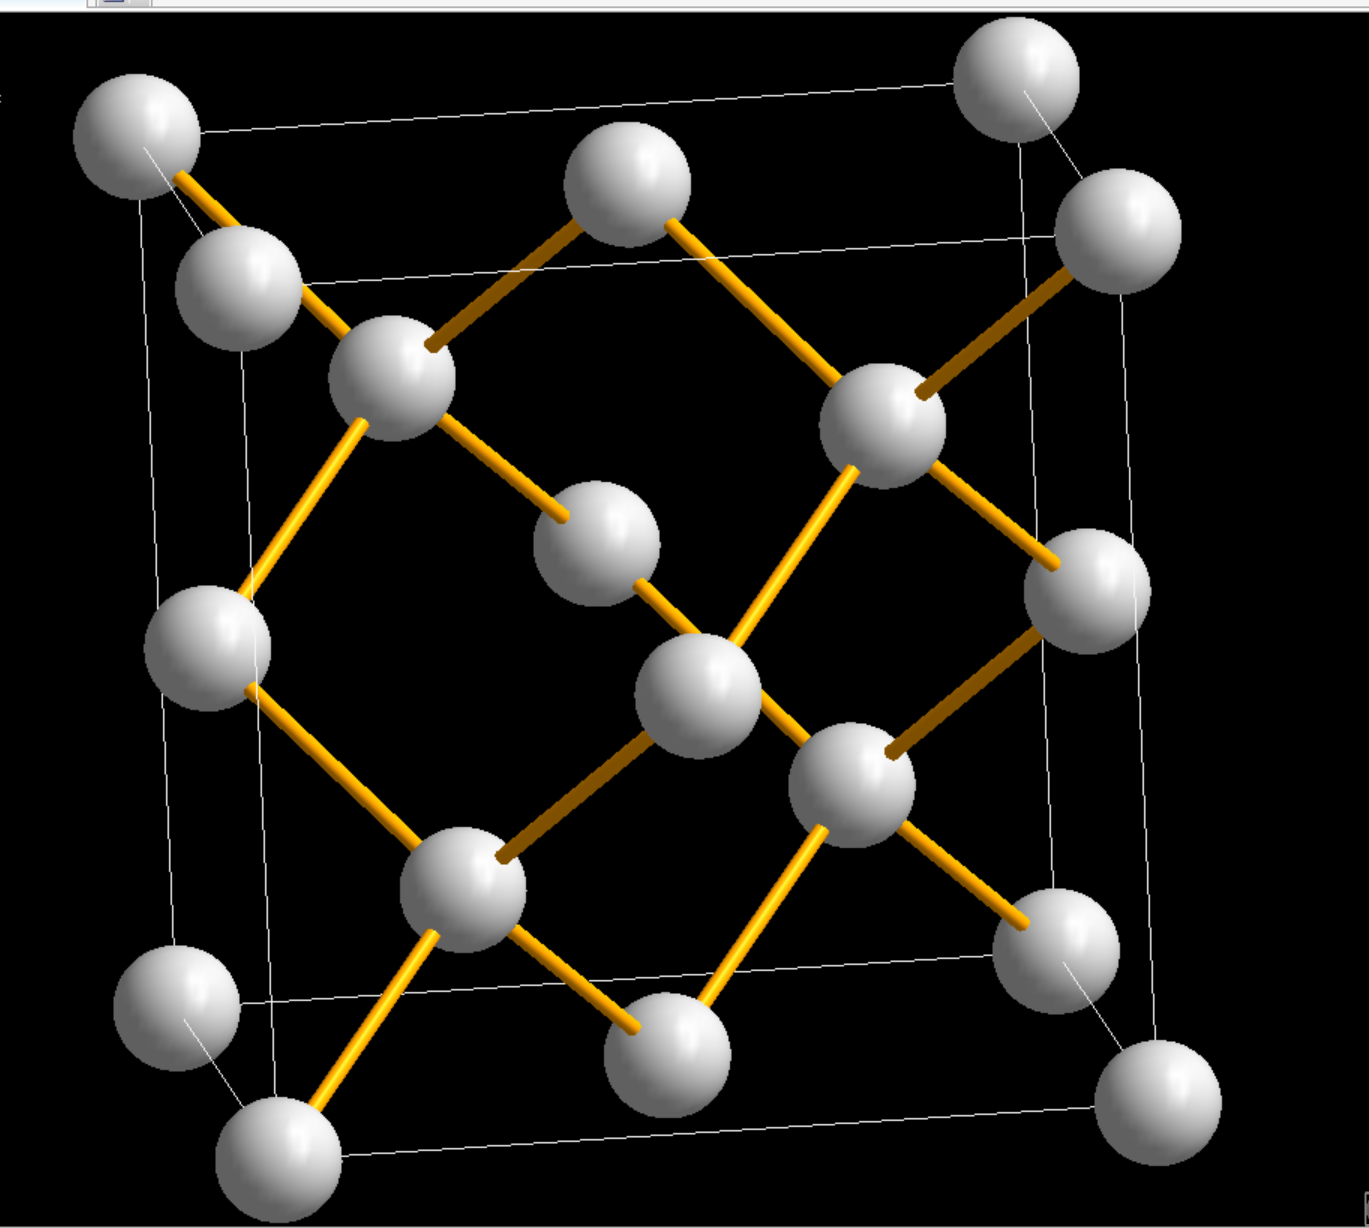
\includegraphics[width=0.5\textwidth]{assets/diamond/c.png}
  \caption{金刚石结构的晶体结构模型（以 Si 为例）}
  \label{fig:diamond-model}
\end{figure}

\begin{figure}[H]
  \centering
  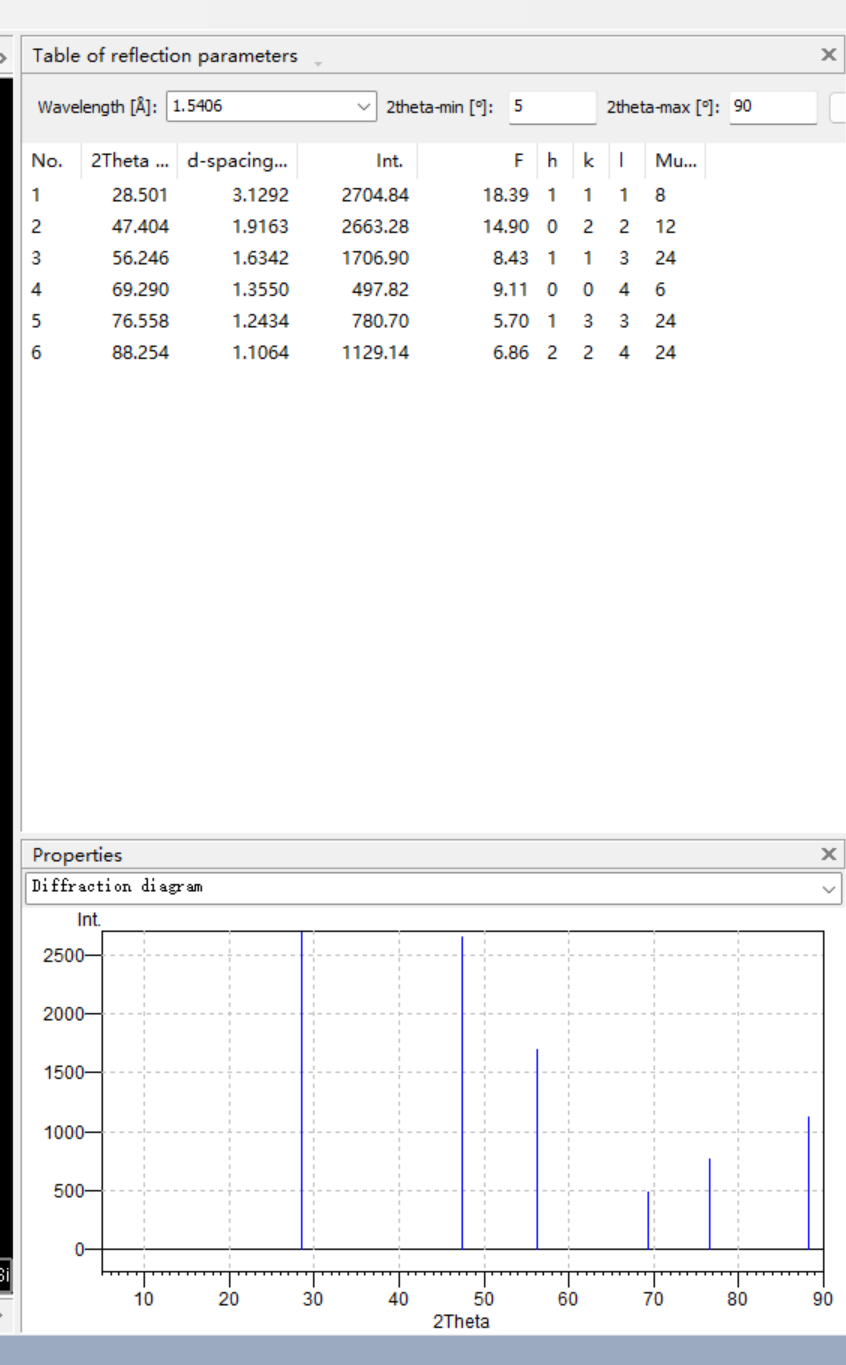
\includegraphics[width=0.4\textwidth]{assets/diamond/d.png}
  \caption{Diamond 模拟的金刚石结构粉末衍射图}
  \label{fig:diamond-xrd}
\end{figure}

\begin{figure}[H]
  \centering
  \subcaptionbox{晶面视图}{%
    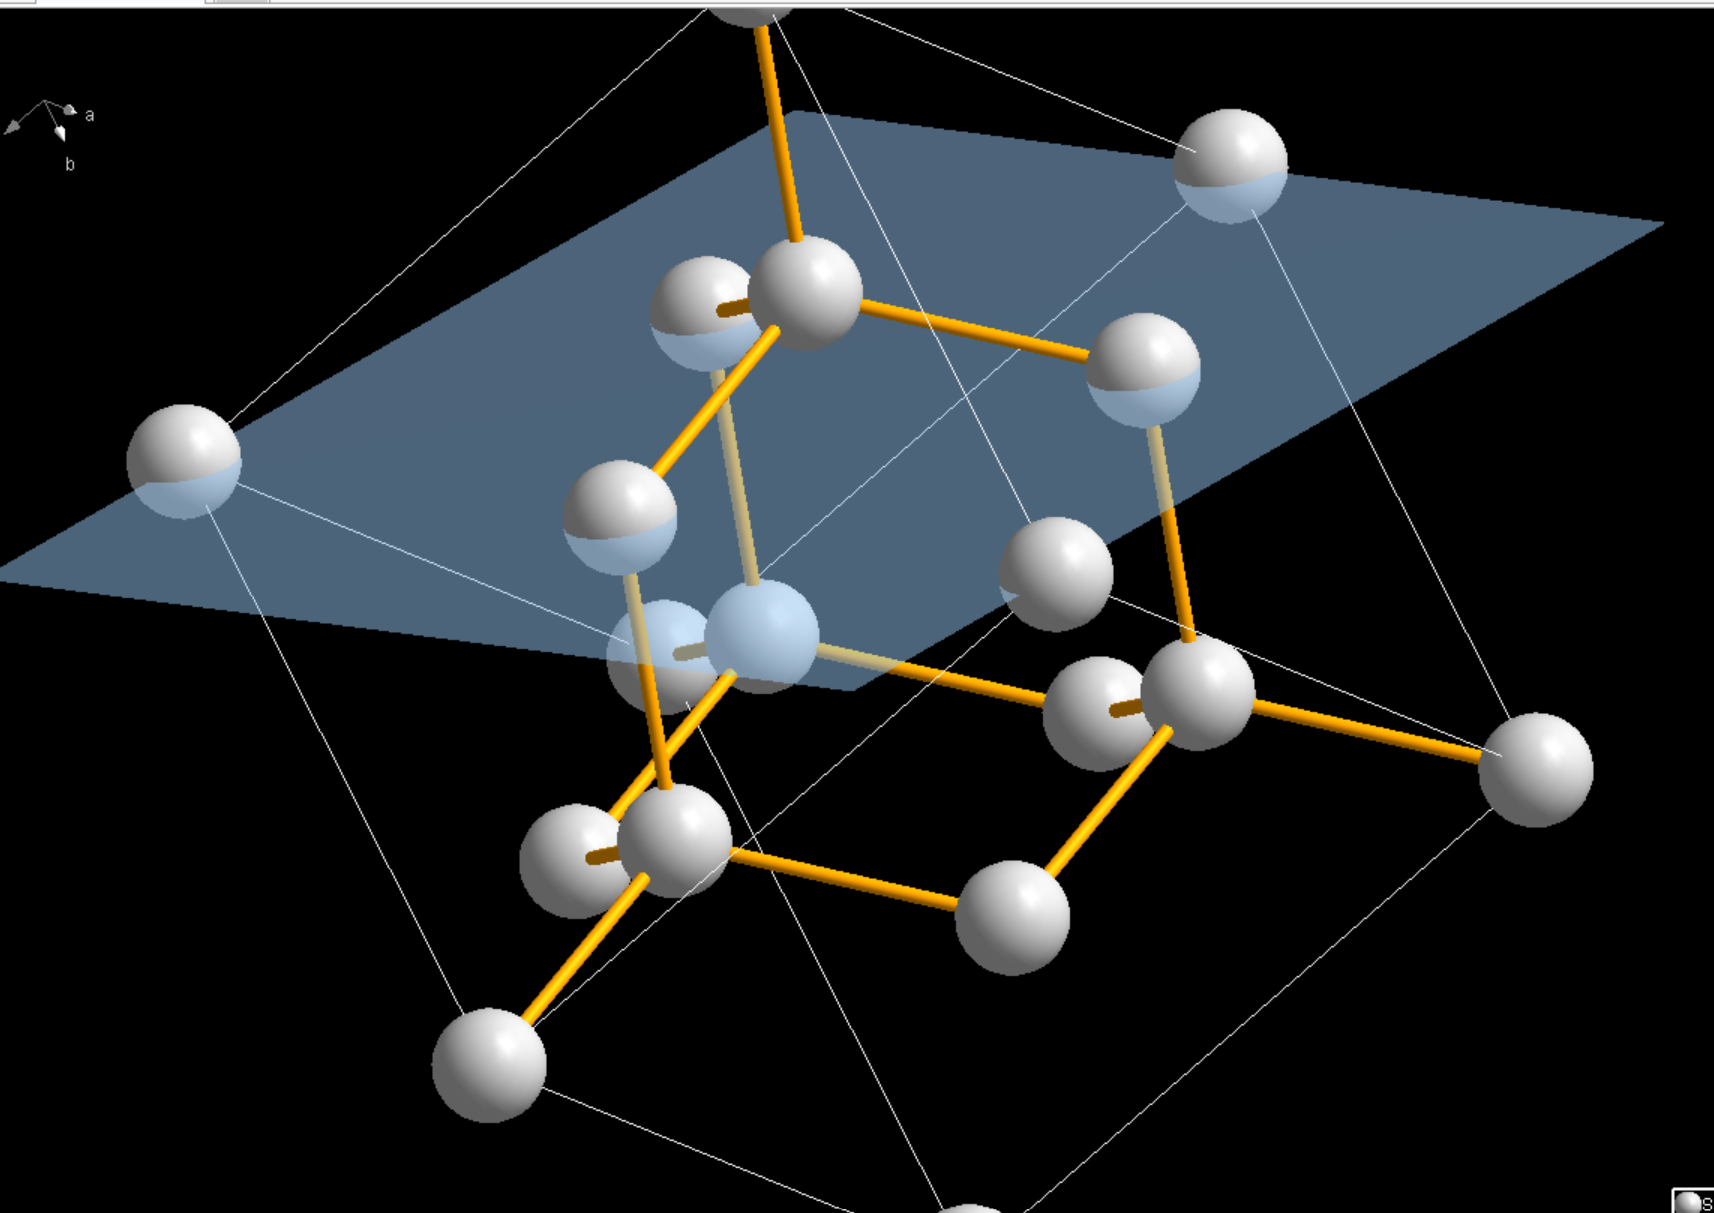
\includegraphics[width=0.44\textwidth]{assets/diamond/e.png}}
  \hfill
  \subcaptionbox{四面体配位（配位数 4）}{%
    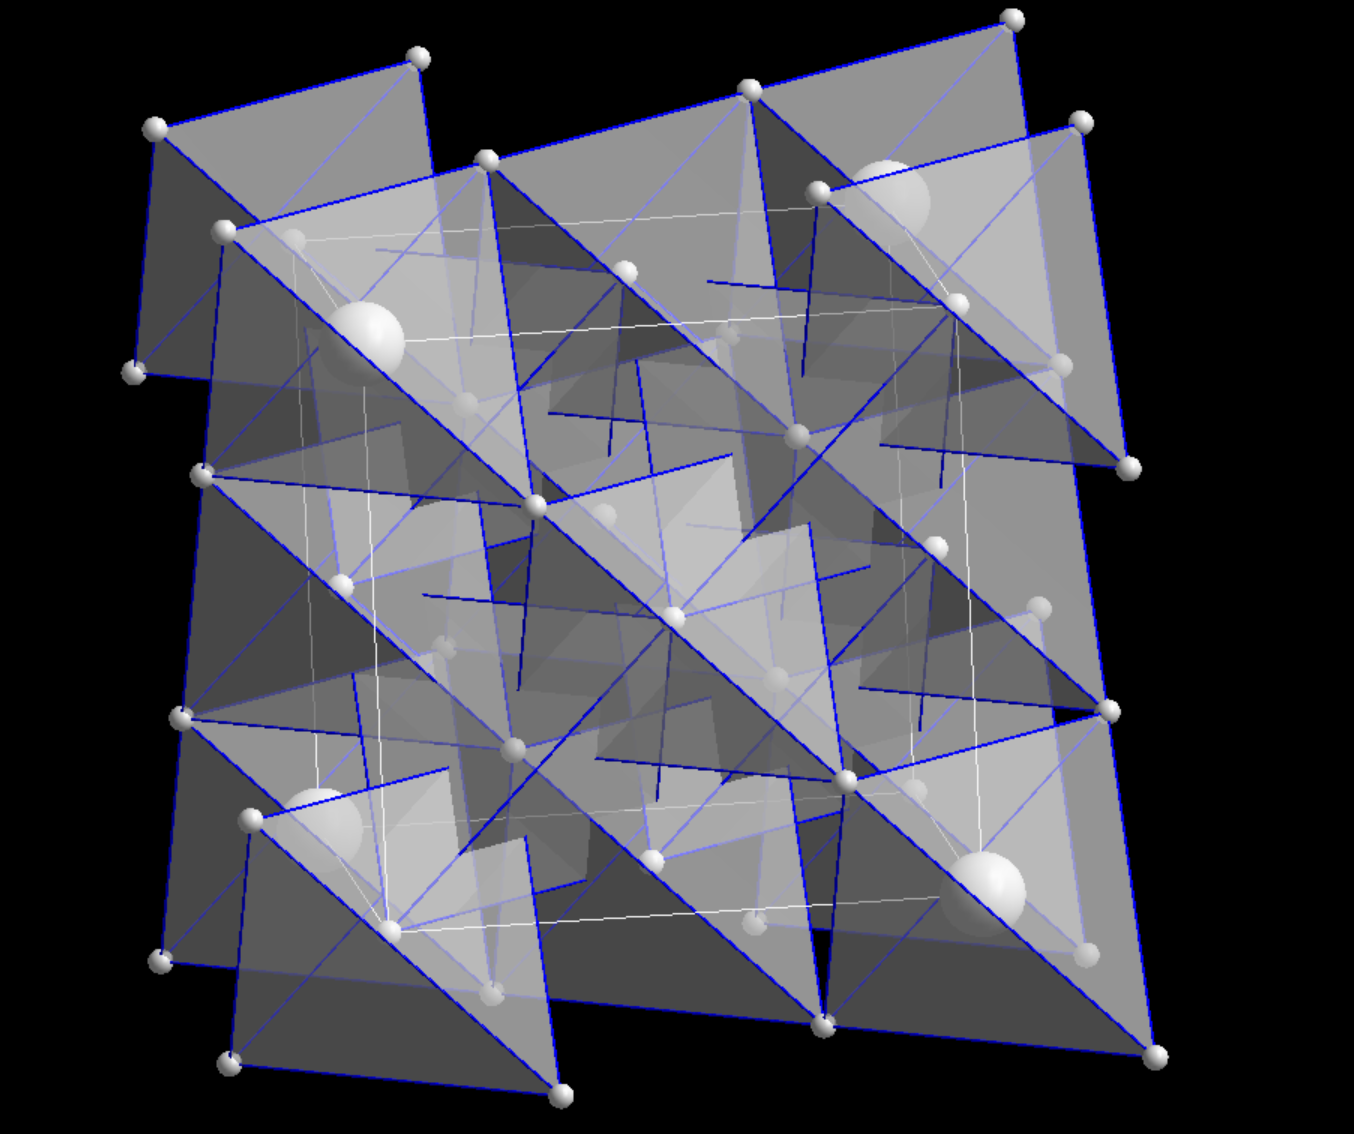
\includegraphics[width=0.44\textwidth]{assets/diamond/f.png}}
  \caption{金刚石结构的晶面与四面体配位}
  \label{fig:diamond-plane}
\end{figure}

\textbf{结构要点。}晶胞内共 8 个原子：4 个在一套 FCC 点阵（顶点与面心）上，另 4 个在
沿体对角线平移 $(1/4,1/4,1/4)$ 的第二套 FCC 点阵上。每个原子与 4 个最近邻以 $sp^3$
杂化轨道成键，构成正四面体配位（图~\ref{fig:diamond-plane}(b)），键角
$109.47^\circ$；最近邻距离（键长）为体对角线的 $1/4$：
\begin{equation}
  d=\frac{\sqrt{3}}{4}a=\frac{\sqrt{3}}{4}\times5.42\approx2.35\ \text{\AA}
\end{equation}
把原子视作沿体对角线相切的刚球（$2r=\sqrt{3}a/4$），堆积因子为
\begin{equation}
  \eta=\frac{8\times\frac{4}{3}\pi\left(\frac{\sqrt{3}}{8}a\right)^3}{a^3}
    =\frac{\pi\sqrt{3}}{16}\approx0.3401
\end{equation}
远低于 FCC 的 $0.7405$。堆积因子的偏小说明结构中存在大量未被占据的空间，这与金刚石
较低的密度（约 $3.5$ g/cm$^3$）相符；其极高的硬度则来自 C--C 共价键的键能与方向性，
两者并不矛盾。$F\,d\,\bar3\,m$ 中的 $d$ 即金刚石滑移面（镜面反映加 $1/4$ 平移），
它把两套 FCC 亚格子联系了起来。

金刚石型结构是共价晶体的典型代表：金刚石（C）是自然界最硬的物质，同型的 Si、Ge 是
最重要的半导体材料，$\alpha$-Sn（灰锡）也属此结构。

% ==================== 2.3.2 小结表 ====================
表~\ref{tab:summary} 汇总了本文建模的八种常见晶体结构的空间群、晶格常数、配位数与
原子堆积因子。

\begin{table}[H]
  \centering
  \small
  \caption{八种常见晶体结构的结构特征汇总}
  \label{tab:summary}
  \begin{tabular}{@{}llllll@{}}
    \toprule
    结构 & 空间群 & 晶格常数（\AA） & $Z$ & 配位数 & 堆积因子 \\
    \midrule
    FCC（Fe） & $F\,m\,\bar3\,m$ & $a=3.43$ & 4 & 12 & 0.7405 \\
    BCC（Fe） & $I\,m\,\bar3\,m$ & $a=2.819$ & 2 & 8（次近邻 6） & 0.6802 \\
    HCP（Mg） & $P\,6_3/m\,m\,c$ & $a=3.2085$，$c=5.2106$ & 2 & 12 & 0.7405（理想） \\
    NaCl & $F\,m\,\bar3\,m$ & $a=5.62$ & 4 & 6 & — \\
    金红石（TiO$_2$） & $P\,4_2/m\,n\,m$ & $a=4.6$，$c=2.9634$ & 2 & 6 & — \\
    锐钛矿（TiO$_2$） & $I\,4_1/a\,m\,d$ & $a=3.784$，$c=9.5146$ & 4 & 6 & — \\
    萤石（CaF$_2$） & $F\,m\,\bar3\,m$ & $a=5.462$ & 4 & Ca：8，F：4 & — \\
    金刚石（Si） & $F\,d\,\bar3\,m$ & $a=5.42$ & 8 & 4 & 0.3401 \\
    \bottomrule
  \end{tabular}
\end{table}

汇总起来看：金属单质以 FCC、BCC、HCP 三种密堆积（或近密堆积）结构为主；离子化合物中，
阴阳离子半径比决定了配位多面体类型（NaCl 六配位、萤石中 Ca 八配位）；共价晶体
（金刚石）以 $sp^3$ 四面体配位为特征，堆积因子最低。八个结构合在一起，勾勒出一条
固定的解读路径：``空间群 + 晶格常数 + 原子占位 $\Rightarrow$ 配位多面体
$\Rightarrow$ 堆积方式''。

% ==================== 2.4 利用 Diamond 软件学习对称元素 ====================
\subsection{利用 Diamond 软件学习对称元素}

2.2.2 节已从理论上介绍了晶体的对称操作与对称元素；本节按照课程要求，进一步利用
Diamond 软件对反演中心、旋转轴、旋转反演轴、镜面、螺旋轴与滑移面六类对称元素逐一
建模仿真，以弄清各对称元素的作用方式、等效位置的生成规律及其在空间群符号中的体现。
各空间群一般位置的等效坐标均参照《国际晶体学表》\cite{hahn2002itt}。

为使对称操作的效果清晰可辨，六组演示采用统一的建模策略：选取能够体现目标对称元素、
且对称操作尽可能简洁的空间群，晶胞内只输入一个位于一般位置（general position）的
Si 原子（分数坐标 $(0.2,\,0.3,\,0.4)$），由 Diamond 按照空间群的对称操作自动生成晶胞内
全部等效原子；通过单胞图与超晶胞图的对比观察原子排布规律，相应的对称操作便一目了然。
操作步骤与 2.3.1 节相同（新建文档 $\to$ 输入空间群与晶格常数 $\to$ 添加原子
$\to$ Build $\to$ Fill $\to$ Unit Cell / Range），观察时的注意事项如下：

\begin{enumerate}[label=（\arabic*）]
  \item 空间群与晶系、晶胞参数的取值必须自洽，晶胞参数按各小节参数表中的演示取值
    输入；
  \item 原子必须位于一般位置：若坐标落入特殊位置（如 $0$、$1/2$、$1/3$ 等），部分
    对称操作会将该原子映射到自身，晶胞内显示的原子数将少于一般位置的等效位置数，
    无法观察到完整的对称操作效果；
  \item 螺旋轴与滑移面含平移分量，只有在超晶胞中才能显示出``旋转（反映）$+$ 平移''
    的复合操作特征；反演中心、旋转轴与旋转反演轴的超晶胞图则用于观察对称操作在
    空间中的周期复现；
  \item 观察时可借助鼠标旋转视图、调整观察方向，并可利用 Add $\to$ Atom Labels
    （ATOM 编号）追踪对称操作前后原子的对应关系。
\end{enumerate}

% ==================== 2.4.1 反演中心 ====================
\subsubsection{反演中心（\texorpdfstring{$P\,\bar1$}{P-1}）}

反演中心（对称中心）$\bar1$ 是一个几何点，操作前后两原子位于同一直线上、关于该点
等距反向。演示反演操作，选对称性最低的中心对称空间群 $P\,\bar1$（No.~2，三斜晶系）
最合适：晶胞中只放一个 Si 原子，参数见表~\ref{tab:sym-inv}。

\begin{table}[H]
  \centering
  \caption{反演中心演示的建模参数}
  \label{tab:sym-inv}
  \begin{tabular}{ll}
    \toprule
    项目 & 参数 \\
    \midrule
    空间群 & $P\,\bar1$（No.~2，三斜晶系） \\
    晶格常数 & $a=b=c=2.0$\,\AA，$\alpha=\beta=90^\circ$，$\gamma=120^\circ$ \\
    原子坐标 & Si：$(0.2,\,0.3,\,0.4)$（一般位置） \\
    等效位置数 & 2（单胞内 2 个原子） \\
    \bottomrule
  \end{tabular}
\end{table}

\begin{figure}[H]
  \centering
  \subcaptionbox{空间群与晶胞参数设置}{%
    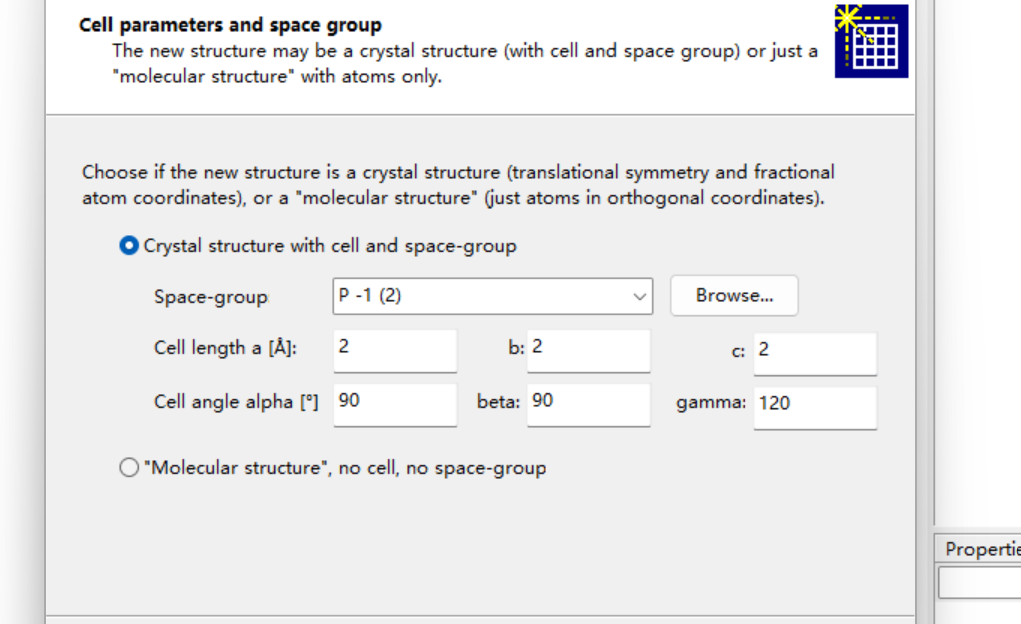
\includegraphics[width=0.44\textwidth]{assets/symmetry/inversion/a.png}}
  \hfill
  \subcaptionbox{非对称单元原子（Si）添加}{%
    \includegraphics[width=0.44\textwidth]{assets/symmetry/inversion/b.png}}
  \caption{反演中心（$P\,\bar1$）演示的参数设置}
  \label{fig:sym-inv-param}
\end{figure}

\begin{figure}[H]
  \centering
  \subcaptionbox{单胞图：2 个原子关于反演中心等距反向}{%
    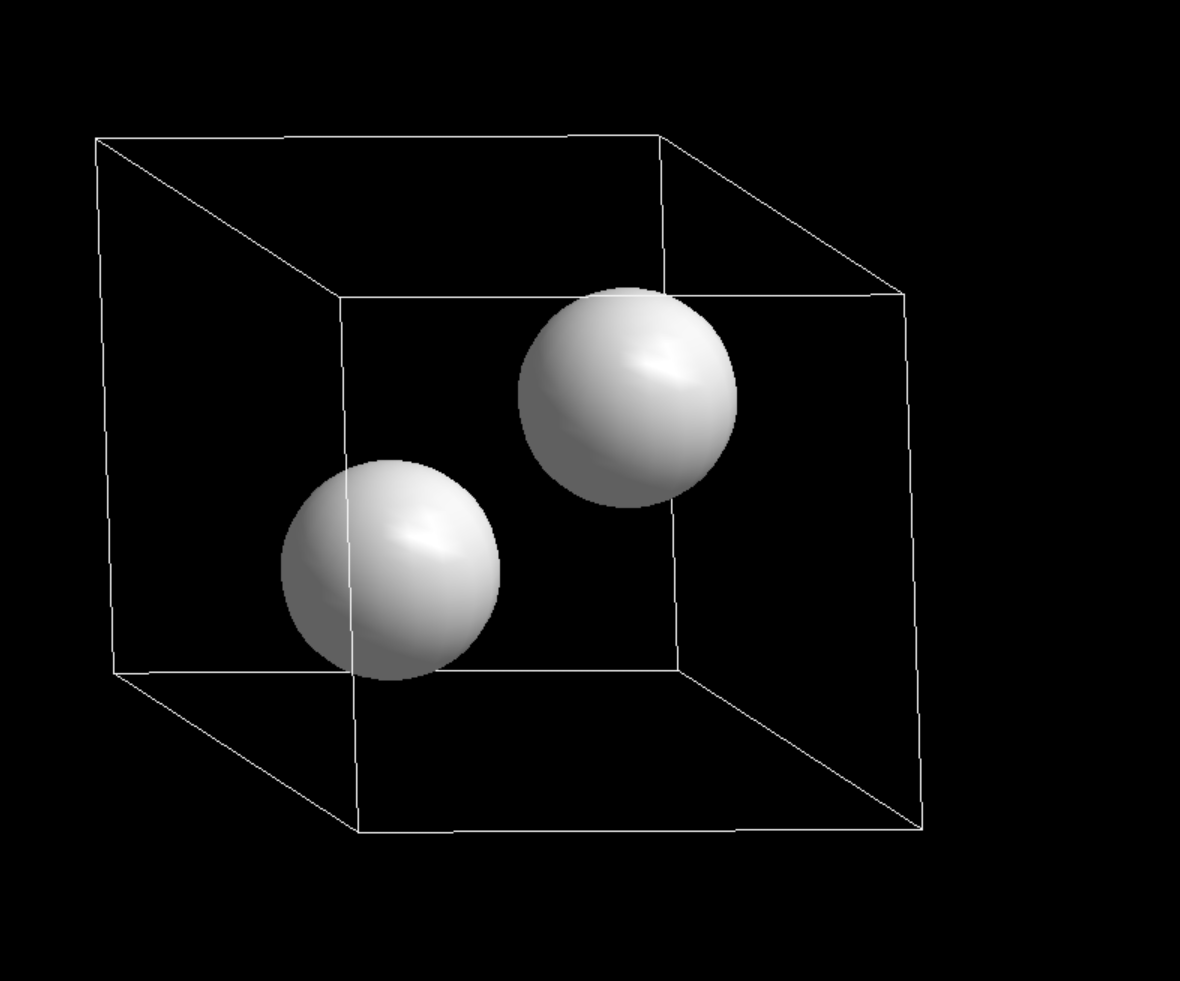
\includegraphics[width=0.44\textwidth]{assets/symmetry/inversion/c.png}}
  \hfill
  \subcaptionbox{超晶胞图：反演对在空间中的周期排列}{%
    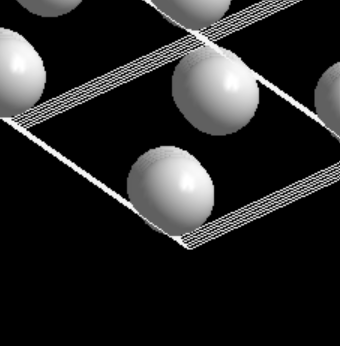
\includegraphics[width=0.44\textwidth]{assets/symmetry/inversion/d.png}}
  \caption{反演中心（$P\,\bar1$）的单胞与超晶胞模型}
  \label{fig:sym-inv-model}
\end{figure}

$P\,\bar1$ 的一般位置等效位置为 $(x,y,z)$ 与 $(\bar x,\bar y,\bar z)$，即全部原子都在
反演操作下``成对''出现：任意一个原子 $(x,y,z)$ 都存在一个与之关于原点等距反向的
配对原子。将 Si 的坐标 $(0.2,0.3,0.4)$ 代入，两个原子的分数坐标为
$(0.2,0.3,0.4)$ 与 $(0.8,0.7,0.6)$，分居晶胞体对角线的两端
（图~\ref{fig:sym-inv-model}(a)）；在超晶胞中，这些反演对沿三个方向周期重复
（图~\ref{fig:sym-inv-model}(b)）。

\textbf{辨认要点。}反演操作的特征很好辨认：原子``成对、共线、等距反向''，单胞内
原子数必为偶数（本例为 2），且每个原子都能找到关于中心等距反向的配对原子。作为
对照，若改用不含任何对称元素的 $P\,1$ 空间群输入同一坐标，晶胞内只会出现 1 个原子，
其位置不受任何对称约束；两个空间群符号 1 与 $\bar1$ 的差别就体现在这里。反演
中心在衍射实验上也有明确后果：中心对称晶体的衍射强度严格满足 Friedel 定律
$I_{hkl}=I_{\bar h\bar k\bar l}$；当晶体不含反演中心时，在发生反常散射（波长接近
元素吸收边）的条件下会出现与 Friedel 定律的偏离，可据此辅助判断反演中心是否存在。

% ==================== 2.4.2 三重旋转轴 ====================
\subsubsection{三重旋转轴（\texorpdfstring{$P\,3$}{P3}）}

旋转轴 $n$ 是一条几何直线：晶体绕它每转 $2\pi/n$ 就复原，转满 $n$ 次后原子回到原处。
要观察 3 次轴，可选用 $c$ 轴为 3 次轴的空间群 $P\,3$（No.~143，三方晶系）；晶胞参数
与原子坐标见表~\ref{tab:sym-rot3}。

\begin{table}[H]
  \centering
  \caption{三重旋转轴演示的建模参数}
  \label{tab:sym-rot3}
  \begin{tabular}{ll}
    \toprule
    项目 & 参数 \\
    \midrule
    空间群 & $P\,3$（No.~143，三方晶系） \\
    晶格常数 & $a=b=c=2.0$\,\AA，$\alpha=\beta=90^\circ$，$\gamma=120^\circ$ \\
    原子坐标 & Si：$(0.2,\,0.3,\,0.4)$（一般位置） \\
    等效位置数 & 3（单胞内 3 个原子） \\
    \bottomrule
  \end{tabular}
\end{table}

\begin{figure}[H]
  \centering
  \subcaptionbox{空间群与晶胞参数设置}{%
    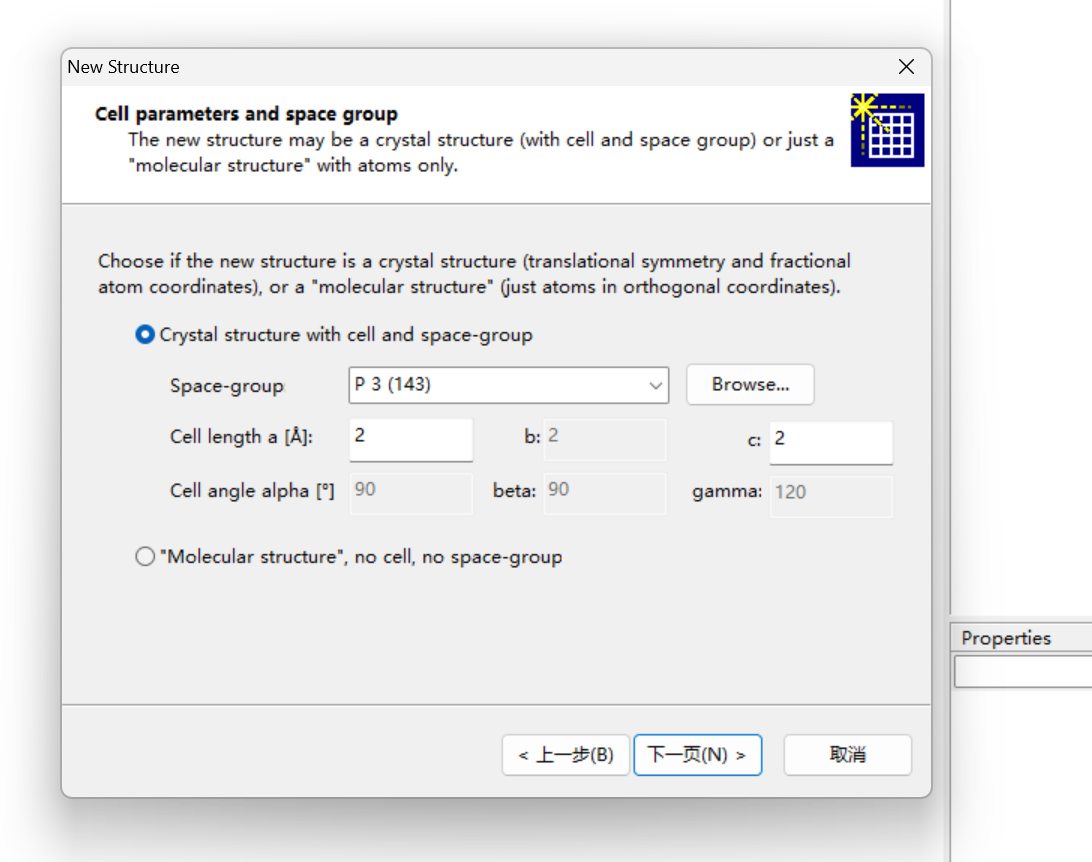
\includegraphics[width=0.44\textwidth]{assets/symmetry/rotation3/a.png}}
  \hfill
  \subcaptionbox{非对称单元原子（Si）添加}{%
    \includegraphics[width=0.44\textwidth]{assets/symmetry/rotation3/b.png}}
  \caption{三重旋转轴（$P\,3$）演示的参数设置}
  \label{fig:sym-rot3-param}
\end{figure}

\begin{figure}[H]
  \centering
  \subcaptionbox{单胞图：3 个原子绕 $c$ 轴呈 $120^\circ$ 分布、位于同一平面}{%
    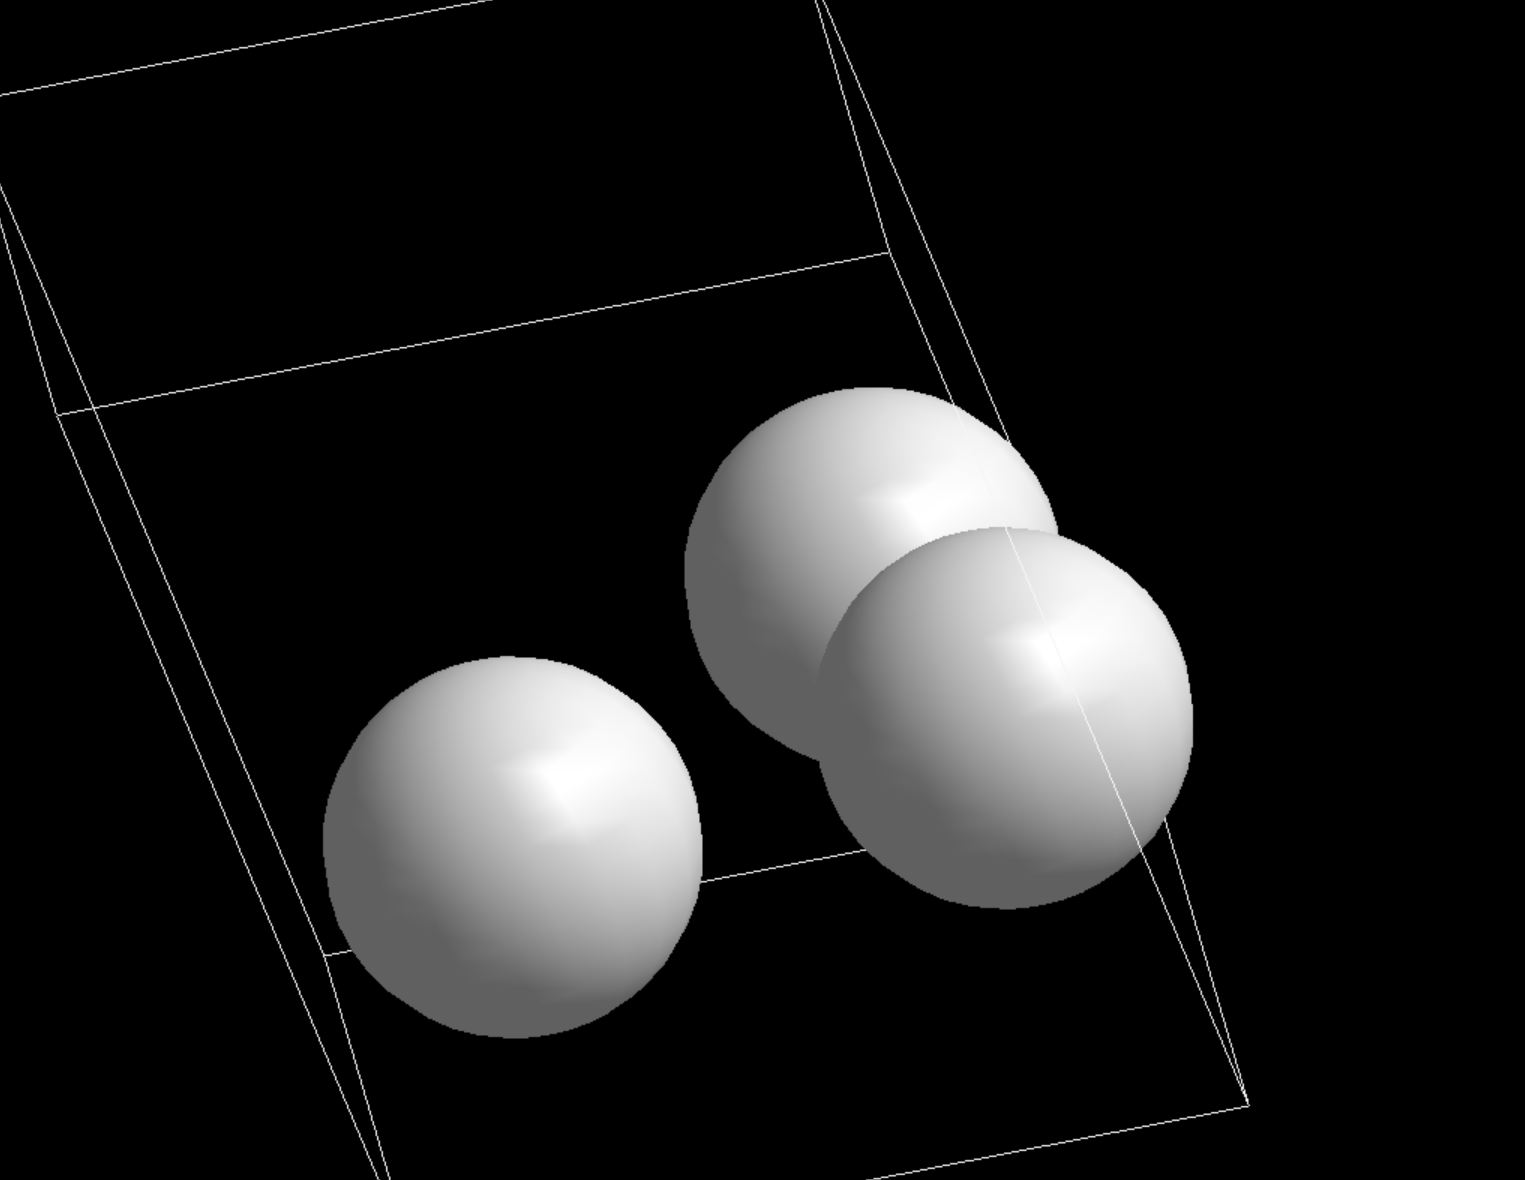
\includegraphics[width=0.44\textwidth]{assets/symmetry/rotation3/c.png}}
  \hfill
  \subcaptionbox{超晶胞图：三重对称花样的周期复现}{%
    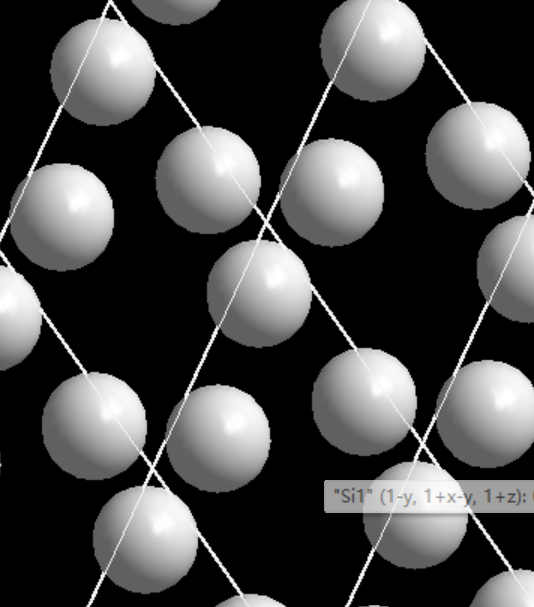
\includegraphics[width=0.44\textwidth]{assets/symmetry/rotation3/d.png}}
  \caption{三重旋转轴（$P\,3$）的单胞与超晶胞模型}
  \label{fig:sym-rot3-model}
\end{figure}

$P\,3$ 的一般位置等效位置为 $(x,y,z)$、$(\bar y,\,x-y,\,z)$ 与 $(-x+y,\,\bar x,\,z)$，
即每次绕 $c$ 轴旋转 $120^\circ$ 得到下一个原子，旋转三次后回到初始位置。将 Si 的
坐标 $(0.2,0.3,0.4)$ 代入，三个原子的分数坐标为 $(0.2,0.3,0.4)$、$(0.7,0.9,0.4)$ 与
$(0.1,0.8,0.4)$：三者 $z$ 坐标相同，位于垂直于 $c$ 轴的同一平面内，且绕 $c$ 轴依次
相距 $120^\circ$（图~\ref{fig:sym-rot3-model}(a)）；在超晶胞中，三重对称花样
沿各方向周期复现（图~\ref{fig:sym-rot3-model}(b)）。

\textbf{一个容易混淆的对照。}$n$ 重旋转轴给出 $n$ 个等效原子，且全部落在垂直于轴的
同一平面内。受晶格周期性限制，晶体中只可能存在 1、2、3、4、6 次旋转轴（见
2.2.2 节），3 次轴是三方晶系的特征对称元素。要注意的是，由旋转轴联系起来的原子只有
``绕轴旋转''的关系，不涉及沿轴方向的平移；把这层关系再加上一个平移分量，得到的就是
2.4.5 节要演示的螺旋轴。

% ==================== 2.4.3 三重旋转反演轴 ====================
\subsubsection{三重旋转反演轴（\texorpdfstring{$P\,\bar3$}{P-3}）}

旋转反演轴 $\bar n$ 是一条几何直线，其操作为旋转 $2\pi/n$ 与反演 $\bar1$ 的联合操作
（先旋转、再反演）。为观察 $\bar3$ 轴，选用空间群 $P\,\bar3$（No.~147，三方晶系，
$\bar3$ 轴沿 $c$ 方向），建模参数见表~\ref{tab:sym-rotinv3}。

\begin{table}[H]
  \centering
  \caption{三重旋转反演轴演示的建模参数}
  \label{tab:sym-rotinv3}
  \begin{tabular}{ll}
    \toprule
    项目 & 参数 \\
    \midrule
    空间群 & $P\,\bar3$（No.~147，三方晶系） \\
    晶格常数 & $a=b=c=2.0$\,\AA，$\alpha=\beta=90^\circ$，$\gamma=120^\circ$ \\
    原子坐标 & Si：$(0.2,\,0.3,\,0.4)$（一般位置） \\
    等效位置数 & 6（单胞内 6 个原子） \\
    \bottomrule
  \end{tabular}
\end{table}

\begin{figure}[H]
  \centering
  \subcaptionbox{空间群与晶胞参数设置}{%
    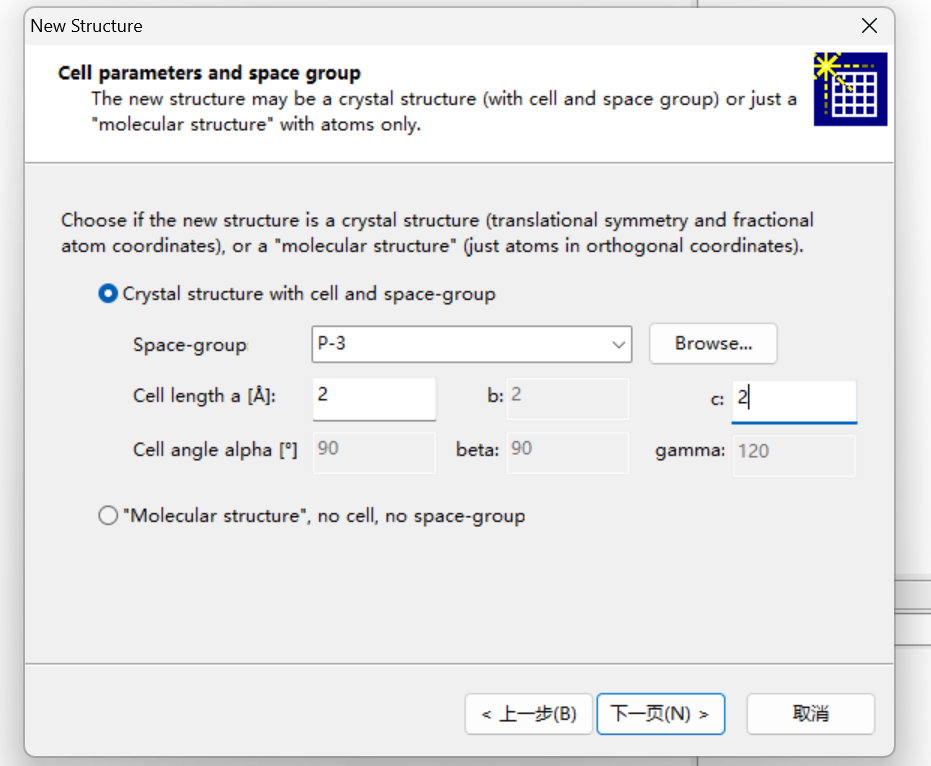
\includegraphics[width=0.44\textwidth]{assets/symmetry/rotoinversion3/a.png}}
  \hfill
  \subcaptionbox{非对称单元原子（Si）添加}{%
    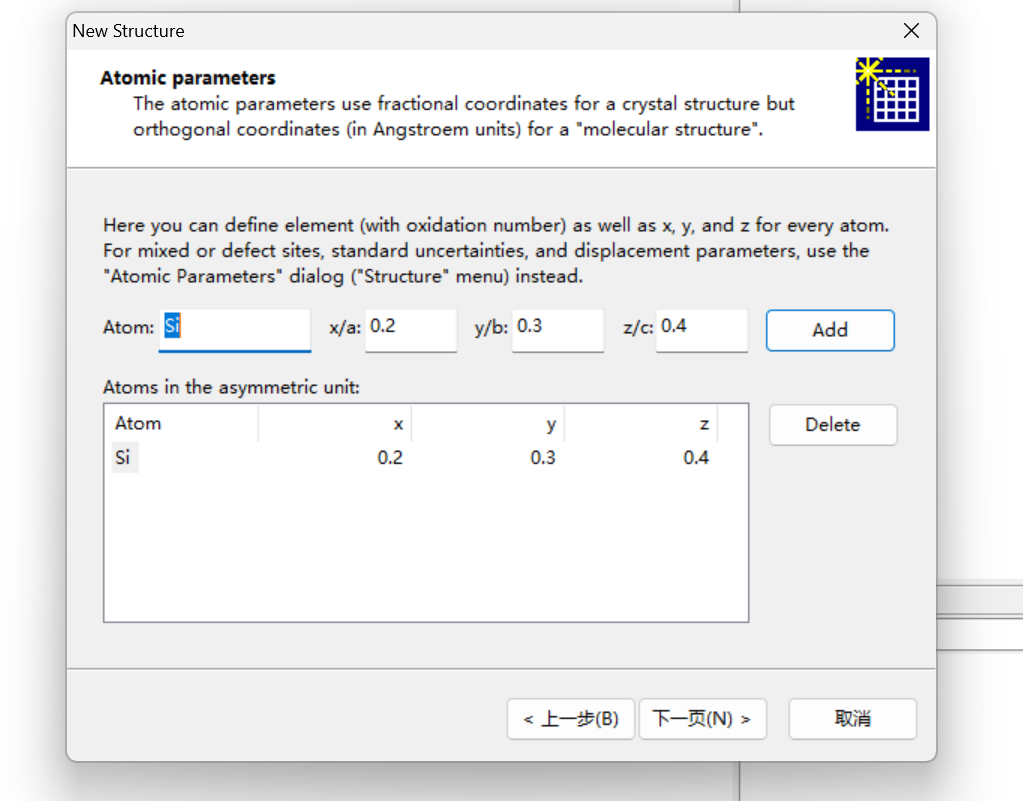
\includegraphics[width=0.44\textwidth]{assets/symmetry/rotoinversion3/b.png}}
  \caption{三重旋转反演轴（$P\,\bar3$）演示的参数设置}
  \label{fig:sym-rotinv3-param}
\end{figure}

\begin{figure}[H]
  \centering
  \subcaptionbox{单胞图：6 个原子分居上下两层（每层 3 个）}{%
    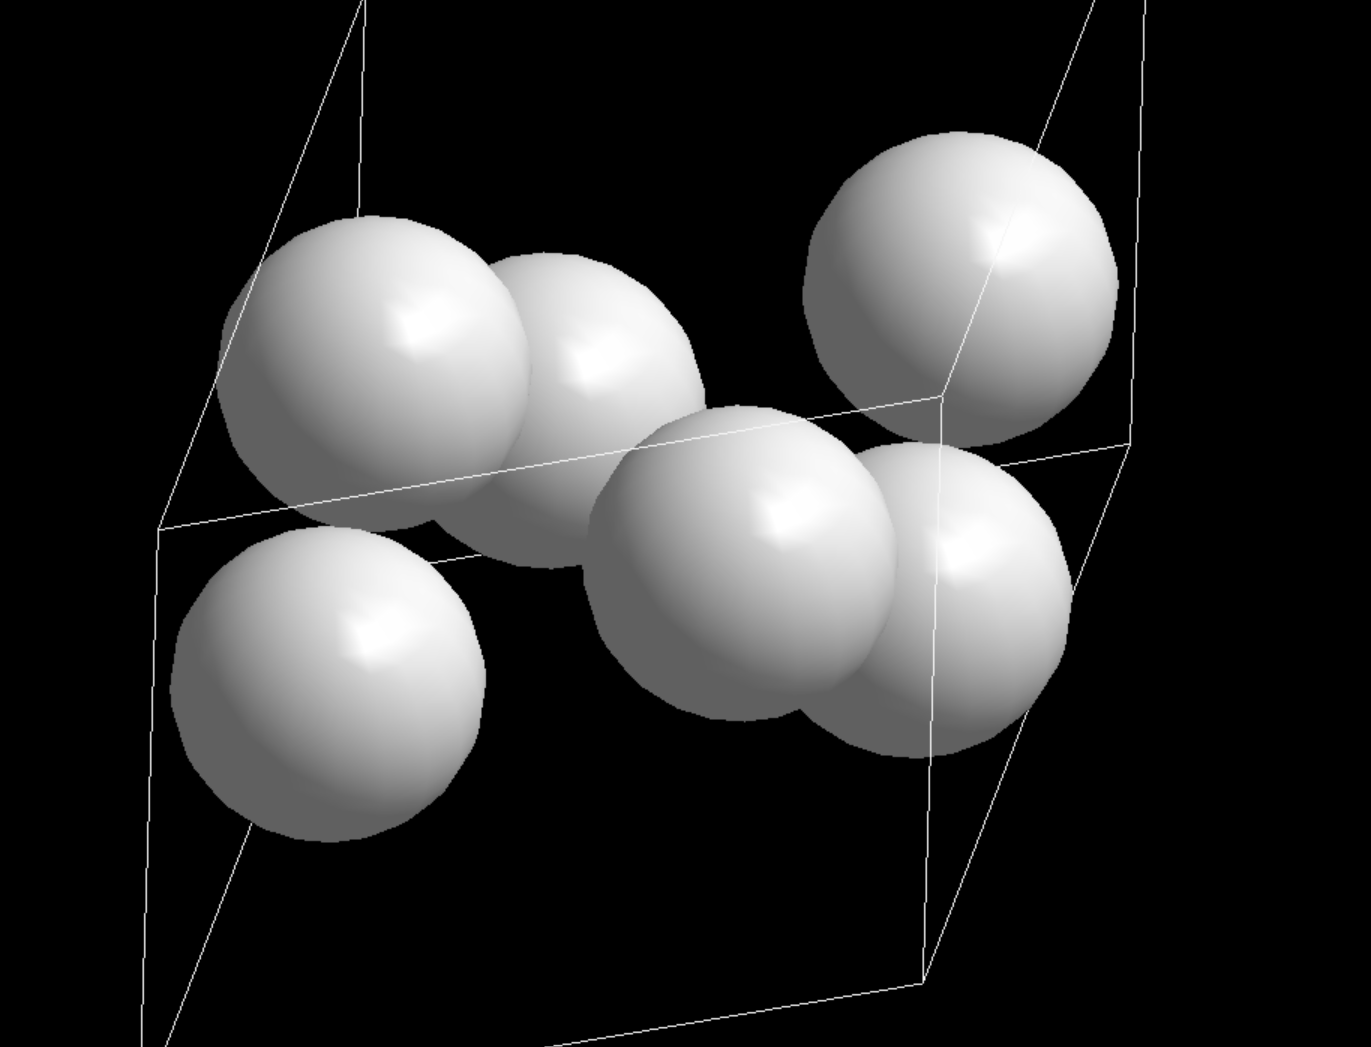
\includegraphics[width=0.44\textwidth]{assets/symmetry/rotoinversion3/c.png}}
  \hfill
  \subcaptionbox{超晶胞图：双层原子组的周期排列}{%
    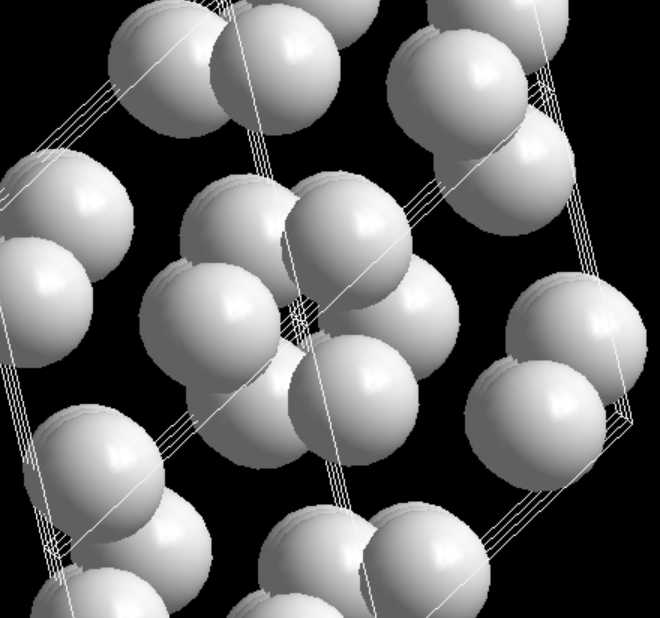
\includegraphics[width=0.44\textwidth]{assets/symmetry/rotoinversion3/d.png}}
  \caption{三重旋转反演轴（$P\,\bar3$）的单胞与超晶胞模型}
  \label{fig:sym-rotinv3-model}
\end{figure}

$P\,\bar3$ 的一般位置等效位置为
\begin{equation}
  \begin{aligned}
    \bar3:\quad &(x,y,z),\quad (\bar y,\,x-y,\,z),\quad (-x+y,\,\bar x,\,z);\\
    &(\bar x,\,\bar y,\,\bar z),\quad (y,\,-x+y,\,\bar z),\quad (x-y,\,x,\,\bar z)
  \end{aligned}
\end{equation}
上半行是绕 $c$ 轴旋转 $120^\circ$ 得到的 3 个原子（$z$ 不变），下半行是它们逐一反演
得到的 3 个原子。将 Si 的坐标 $(0.2,0.3,0.4)$ 代入，6 个原子的分数坐标为
$(0.2,0.3,0.4)$、$(0.7,0.9,0.4)$、$(0.1,0.8,0.4)$（上层，$z=0.4$）与
$(0.8,0.7,0.6)$、$(0.3,0.1,0.6)$、$(0.9,0.2,0.6)$（下层，$z=0.6$）。可见旋转反演
操作产生的原子不位于同一平面，而是分居上下两层
（图~\ref{fig:sym-rotinv3-model}(a)）；超晶胞中双层原子组沿空间周期排列
（图~\ref{fig:sym-rotinv3-model}(b)）。因此，$\bar3$ 等效于 $3+\bar1$ 的联合：先经
3 次轴旋转得到 3 个原子，再经反演得到另外 3 个原子。

\textbf{特征与辨识要点。}$\bar3$ 的完整联合操作需依次进行 6 次才能回到初始位置，
故单胞内出现 6 个（而不是 3 个）等效原子——操作次数为 6 而非 3，这是旋转反演轴的
特有性质。若从平行于 $\bar3$ 轴的方向观察，6 个原子看似呈六重对称分布，容易与
6 次旋转轴混淆；两者的区别在于：旋转反演产生的原子分居上下两层、两层之间存在
反演对应关系，而 6 次旋转轴产生的 6 个原子位于垂直轴的同一平面内。$\bar3$ 是
立方晶系沿体对角线方向的特征对称元素（如 $F\,m\,\bar3\,m$ 中的 $\bar3$）。

% ==================== 2.4.4 镜面 ====================
\subsubsection{镜面（\texorpdfstring{$P\,m\,\bar3$}{Pm-3}）}

镜面 $m$ 是一个对称平面，其操作前后两原子位于镜面同一法向的两侧、等距反向。为观察
镜面操作，选用空间群 $P\,m\,\bar3$（No.~200，立方晶系）：其点群 $m\,\bar3$ 由 3 组
互相垂直的镜面、4 个沿体对角线的 3 次轴、3 个 2 次轴及反演中心组合而成，其中镜面
垂直于三个晶轴方向，便于观察原子的镜像成对关系。建模参数见表~\ref{tab:sym-mir}。

\begin{table}[H]
  \centering
  \caption{镜面演示的建模参数}
  \label{tab:sym-mir}
  \begin{tabular}{ll}
    \toprule
    项目 & 参数 \\
    \midrule
    空间群 & $P\,m\,\bar3$（No.~200，立方晶系） \\
    晶格常数 & $a=b=c=5.0$\,\AA，$\alpha=\beta=\gamma=90^\circ$ \\
    原子坐标 & Si：$(0.2,\,0.3,\,0.4)$（一般位置） \\
    等效位置数 & 24（单胞内 24 个原子） \\
    \bottomrule
  \end{tabular}
\end{table}

\begin{figure}[H]
  \centering
  \subcaptionbox{空间群与晶胞参数设置}{%
    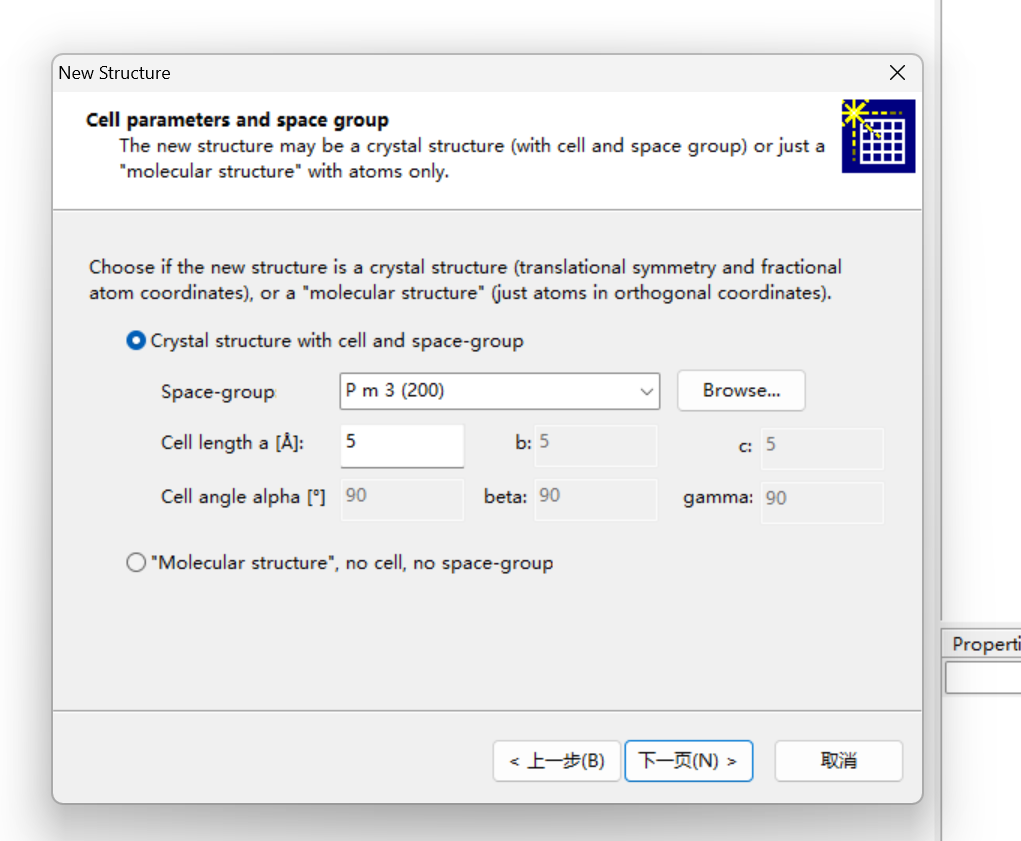
\includegraphics[width=0.44\textwidth]{assets/symmetry/mirror/a.png}}
  \hfill
  \subcaptionbox{非对称单元原子（Si）添加}{%
    \includegraphics[width=0.44\textwidth]{assets/symmetry/mirror/b.png}}
  \caption{镜面（$P\,m\,\bar3$）演示的参数设置}
  \label{fig:sym-mir-param}
\end{figure}

\begin{figure}[H]
  \centering
  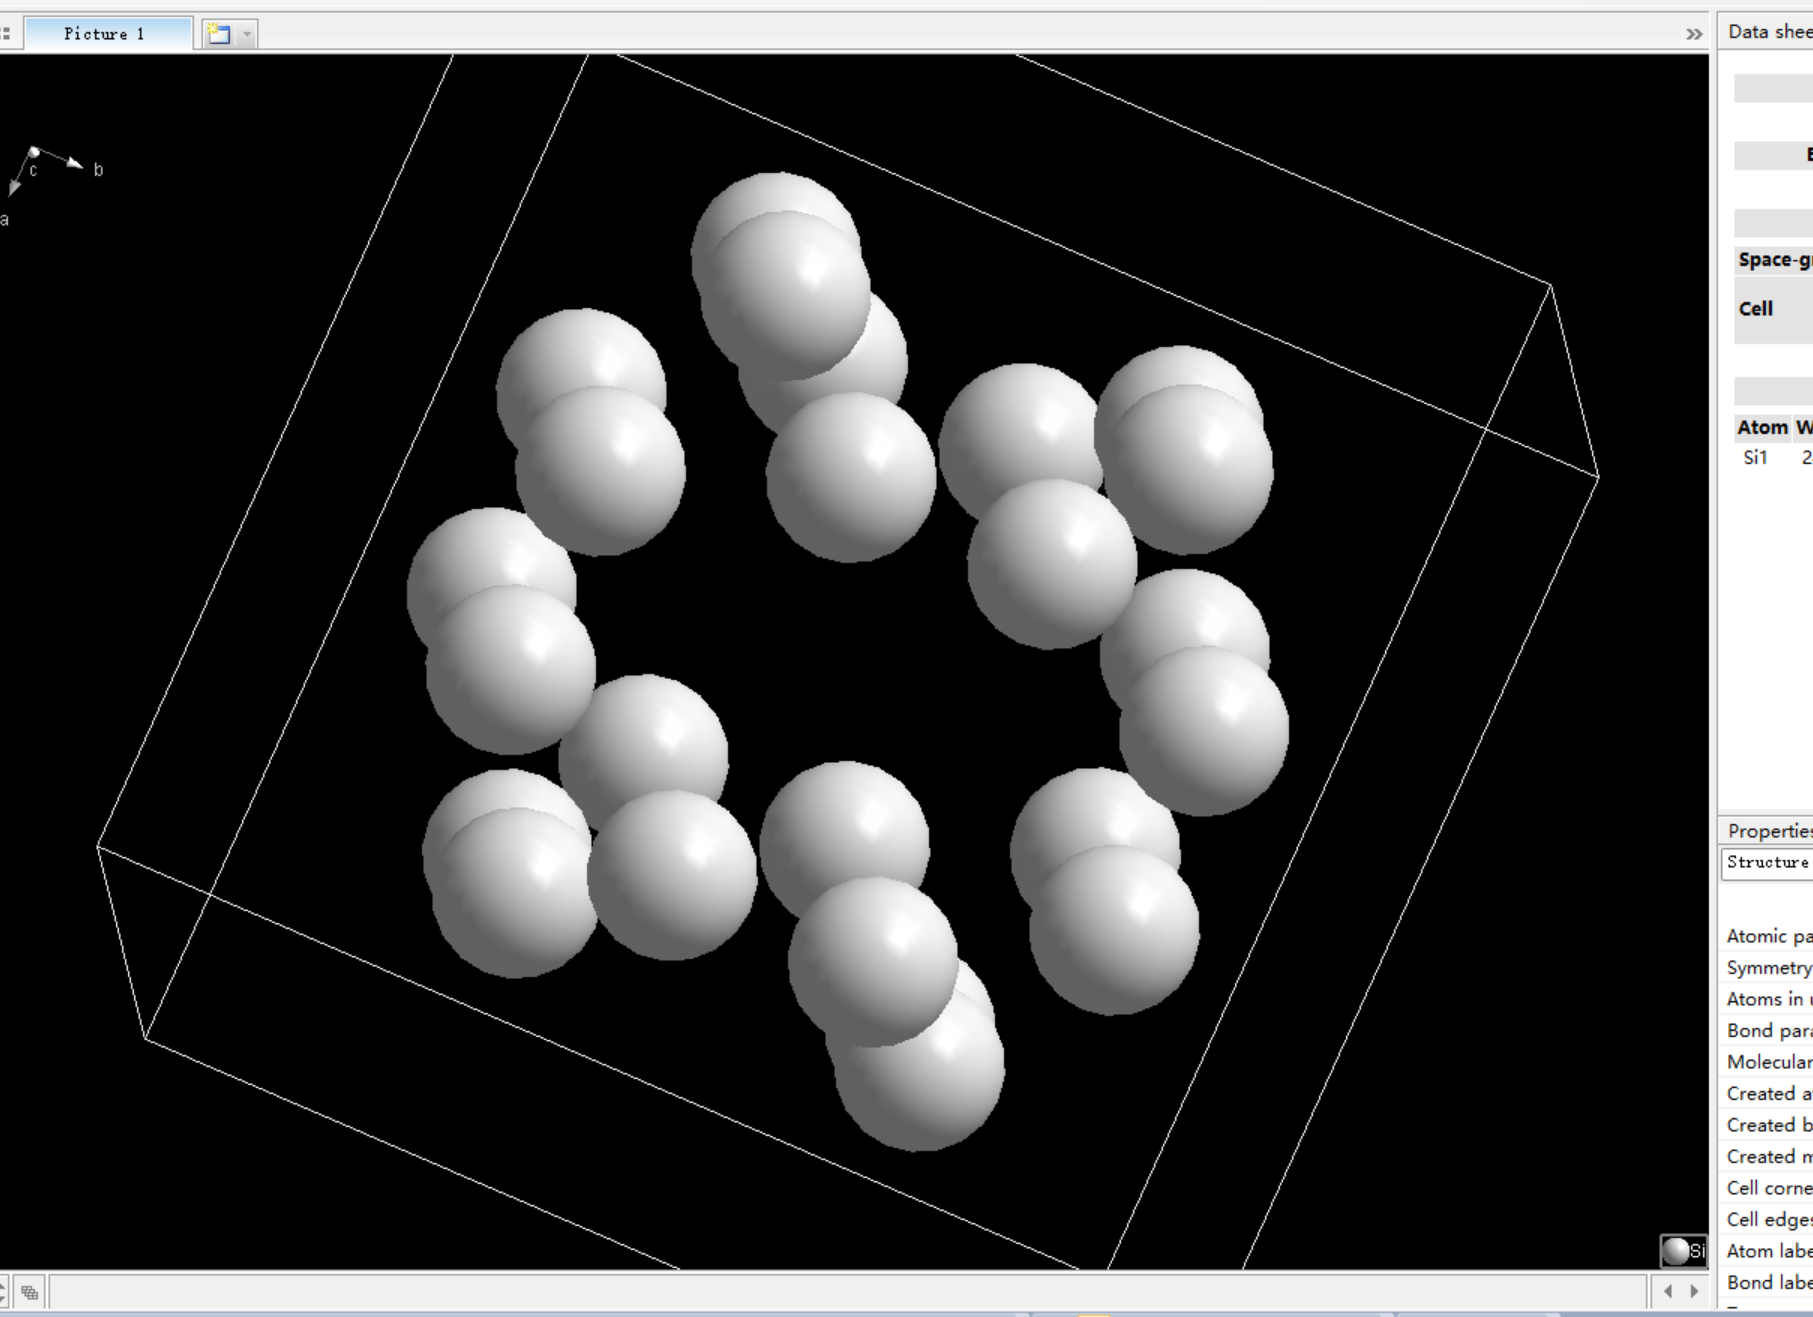
\includegraphics[width=0.5\textwidth]{assets/symmetry/mirror/c.png}
  \caption{镜面（$P\,m\,\bar3$）的单胞模型：24 个等效原子关于三组互相垂直的镜面
    镜像分布}
  \label{fig:sym-mir-model}
\end{figure}

$P\,m\,\bar3$ 中垂直于三个晶轴的镜面操作可分别写为
\begin{equation}
  \begin{aligned}
    m_{\perp a}:\ (x,y,z)\to(\bar x,\,y,\,z),&\qquad
    m_{\perp b}:\ (x,y,z)\to(x,\,\bar y,\,z),\\
    m_{\perp c}:\ (x,y,z)\to(x,\,y,\,\bar z).&
  \end{aligned}
\end{equation}
以 Si 的坐标 $(0.2,0.3,0.4)$ 为例，其关于三个镜面的像分别为 $(0.8,0.3,0.4)$、
$(0.2,0.7,0.4)$ 与 $(0.2,0.3,0.6)$。这些镜面操作与 4 个 3 次轴（体对角线方向）、
3 个 2 次轴、反演中心相互组合，在单胞内共生成 24 个等效原子
（图~\ref{fig:sym-mir-model}）。由于 24 个原子在晶胞内间距较小，图中原子显得较为
密集；实际观察时可旋转模型并利用 Atom Design 适当减小原子显示半径，即可清晰看到
原子关于镜面的成对镜像关系。

\textbf{特征与辨识要点。}镜面操作的显著特征是原子``镜像成对''：每组原子对位于镜面
两侧、与镜面等距且连线垂直于镜面。镜面不含任何平移分量，属宏观对称元素，镜面操作
还可以等效地记为 $\bar2$（二次旋转反演轴）。在 $P\,m\,\bar3$ 中，三组镜面互相垂直，
分别垂直于 $a$、$b$、$c$ 轴；镜面与 3 次轴、2 次轴及反演中心的组合使一般位置的多
重度达到 24。与镜面外形相似但含平移分量的对称元素是滑移面（见 2.4.6 节），两者的
区别只有在观察超晶胞时才能直接看出。

% ==================== 2.4.5 三重螺旋轴 ====================
\subsubsection{三重螺旋轴（\texorpdfstring{$P\,3_1$}{P3₁}）}

螺旋轴 $n_m$ 为旋转 $2\pi/n$ 与沿轴平移 $m/n$ 个晶格周期的联合操作，是典型的微观
对称元素。演示 $3_1$ 螺旋轴（旋转 $120^\circ$ 加平移 $1/3$ 周期），选用空间群
$P\,3_1$（No.~144，三方晶系）；参数见表~\ref{tab:sym-screw31}。

\begin{table}[H]
  \centering
  \caption{三重螺旋轴演示的建模参数}
  \label{tab:sym-screw31}
  \begin{tabular}{ll}
    \toprule
    项目 & 参数 \\
    \midrule
    空间群 & $P\,3_1$（No.~144，三方晶系） \\
    晶格常数 & $a=b=c=5.0$\,\AA，$\alpha=\beta=90^\circ$，$\gamma=120^\circ$ \\
    原子坐标 & Si：$(0.2,\,0.3,\,0.4)$（一般位置） \\
    等效位置数 & 3（单胞内 3 个原子，高度各不相同） \\
    \bottomrule
  \end{tabular}
\end{table}

\begin{figure}[H]
  \centering
  \subcaptionbox{空间群与晶胞参数设置}{%
    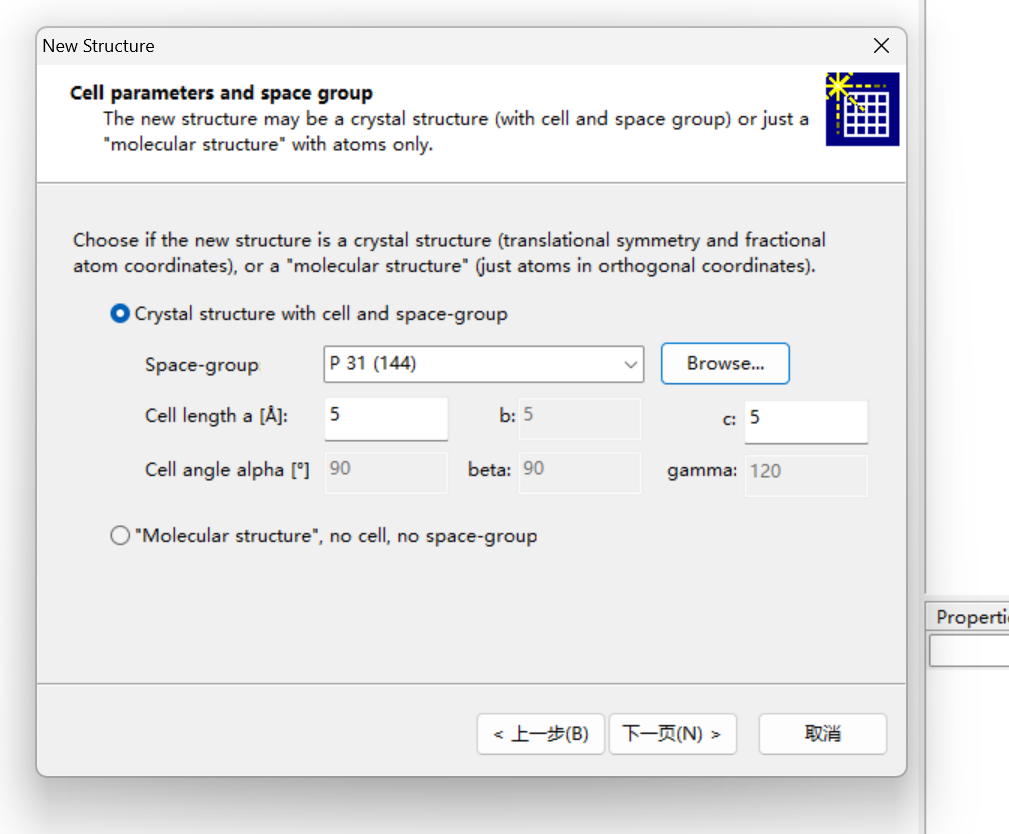
\includegraphics[width=0.44\textwidth]{assets/symmetry/screw31/a.png}}
  \hfill
  \subcaptionbox{非对称单元原子（Si）添加}{%
    \includegraphics[width=0.44\textwidth]{assets/symmetry/screw31/b.png}}
  \caption{三重螺旋轴（$P\,3_1$）演示的参数设置}
  \label{fig:sym-screw31-param}
\end{figure}

\begin{figure}[H]
  \centering
  \subcaptionbox{单胞图：3 个原子高度各不相同、呈螺旋排列}{%
    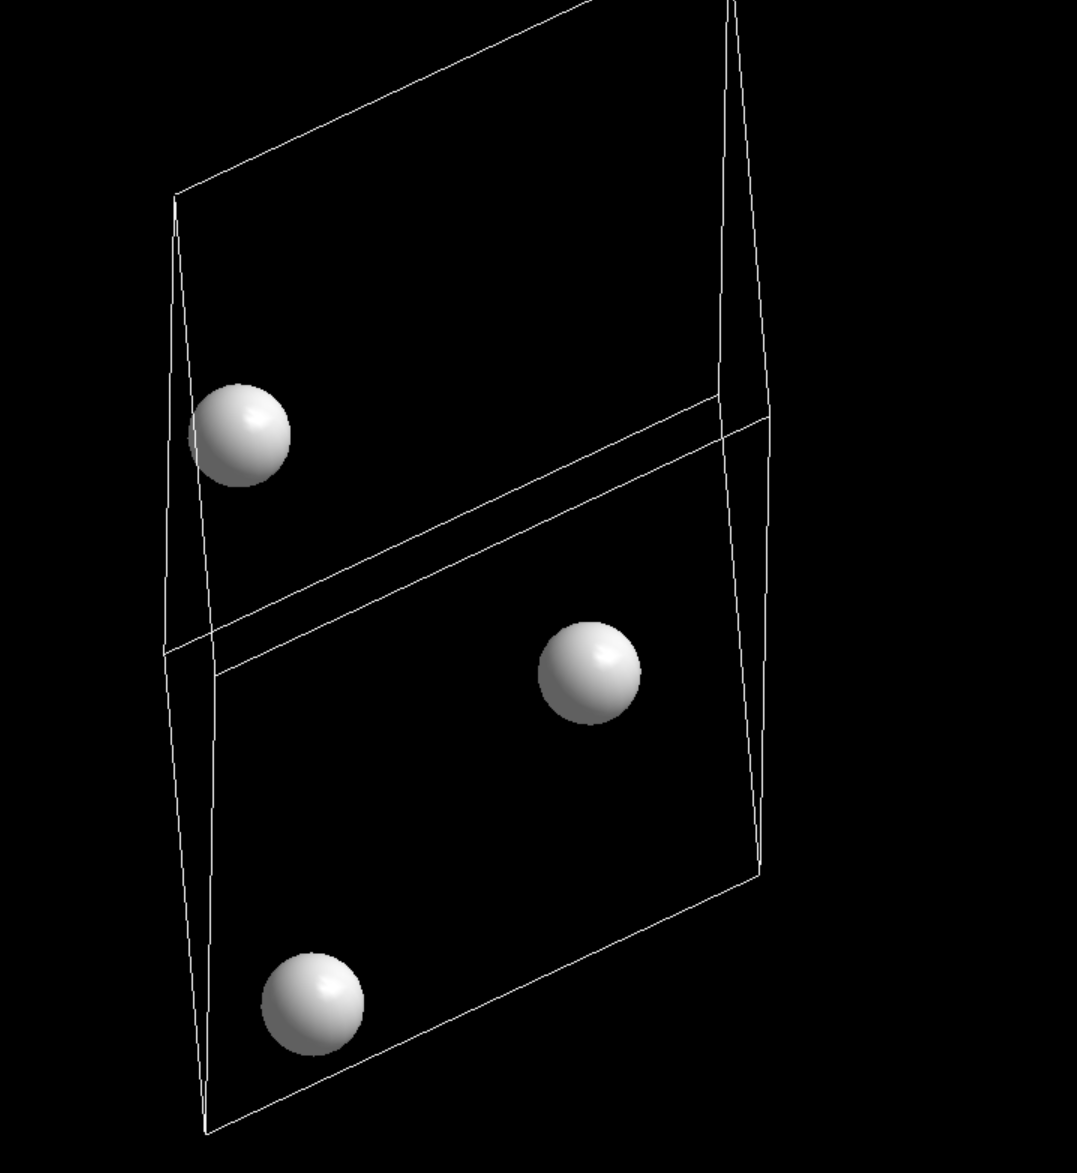
\includegraphics[width=0.44\textwidth]{assets/symmetry/screw31/c.png}}
  \hfill
  \subcaptionbox{超晶胞图：沿 $c$ 轴方向延伸的螺旋链}{%
    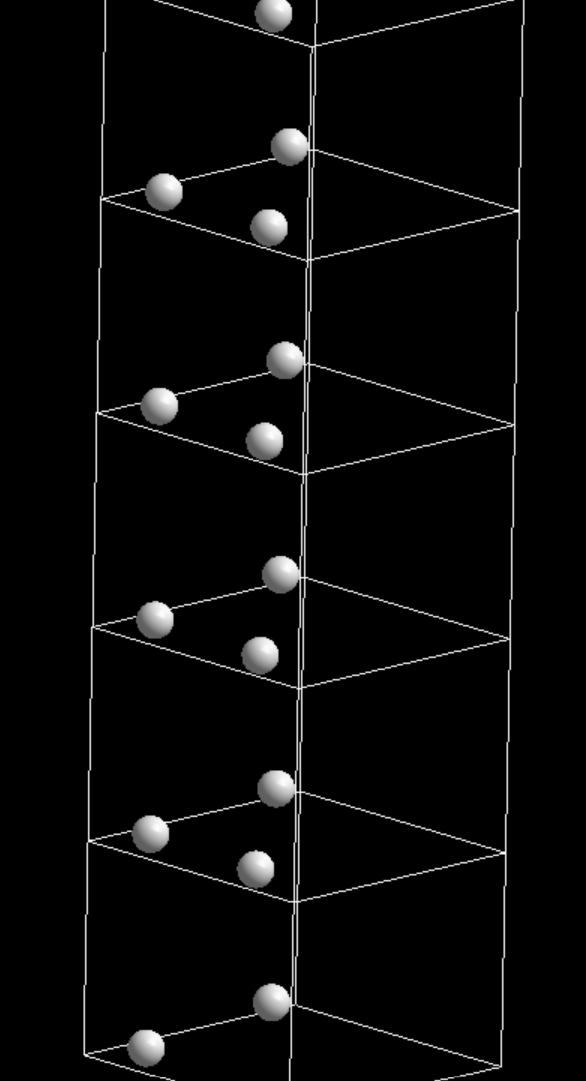
\includegraphics[width=0.44\textwidth]{assets/symmetry/screw31/d.png}}
  \caption{三重螺旋轴（$P\,3_1$）的单胞与超晶胞模型}
  \label{fig:sym-screw31-model}
\end{figure}

$P\,3_1$ 的一般位置等效位置为 $(x,y,z)$、$(\bar y,\,x-y,\,z+\tfrac13)$ 与
$(-x+y,\,\bar x,\,z+\tfrac23)$：操作一次得到 1 个原子，共操作 3 次、生成 3 个原子。
将 Si 的坐标 $(0.2,0.3,0.4)$ 代入，3 个原子的分数坐标为 $(0.2,0.3,0.4)$、
$(0.7,0.9,0.733)$ 与 $(0.1,0.8,0.067)$：三者高度（$z$ 坐标）依次相差 $1/3$，沿 $c$
轴呈螺旋上升排列，不位于同一平面（图~\ref{fig:sym-screw31-model}(a)）；执行第 3 次
操作时，原子回到与初始位置等效的位置 $(0.2,0.3,1.4)$：绕轴旋转一周的同时，沿 $c$
方向平移了 1 个晶胞周期，因此在超晶胞中沿 $c$ 轴可以看到连续的螺旋链
（图~\ref{fig:sym-screw31-model}(b)）。

\textbf{与 3 次旋转轴的对照。}两者的区别只在一条：是否含沿轴方向的平移分量。
3 次旋转轴的 3 个原子位于同一平面（2.4.2 节），而 $3_1$ 螺旋轴的 3 个原子逐个升高
$c/3$、呈螺旋排列。螺旋轴 $n_m$ 的 $m$ 不同，平移分量为 $m/n$ 个周期；$3_1$ 与
$3_2$ 的平移方向与旋转方向组合相反，互为对映关系（右旋与左旋）。螺旋轴属微观对称
元素，只能存在于无限晶体中，实际晶体中十分常见，例如 $\alpha$-石英的 $P\,3_1\,2\,1$
与 $P\,3_2\,2\,1$ 就互为含 $3_1$、$3_2$ 螺旋轴的一对对映空间群。

% ==================== 2.4.6 滑移面 ====================
\subsubsection{滑移面（\texorpdfstring{$P\,1\,c\,1$}{P1c1}）}

滑移面是镜面反映与沿面内特定方向平移的联合操作，属于微观对称元素。为观察 $c$ 滑移面
（滑移方向为 $c$、滑移量为 $1/2$ 个周期），选用空间群 $P\,1\,c\,1$（No.~7，单斜
晶系，镜面垂直于 $b$ 轴），建模参数见表~\ref{tab:sym-glide}。

\begin{table}[H]
  \centering
  \caption{滑移面演示的建模参数}
  \label{tab:sym-glide}
  \begin{tabular}{ll}
    \toprule
    项目 & 参数 \\
    \midrule
    空间群 & $P\,1\,c\,1$（No.~7，单斜晶系） \\
    晶格常数 & $a=b=c=3.0$\,\AA，$\alpha=\beta=\gamma=90^\circ$ \\
    原子坐标 & Si：$(0.2,\,0.3,\,0.4)$（一般位置） \\
    等效位置数 & 2（单胞内 2 个原子） \\
    \bottomrule
  \end{tabular}
\end{table}

\begin{figure}[H]
  \centering
  \subcaptionbox{空间群与晶胞参数设置}{%
    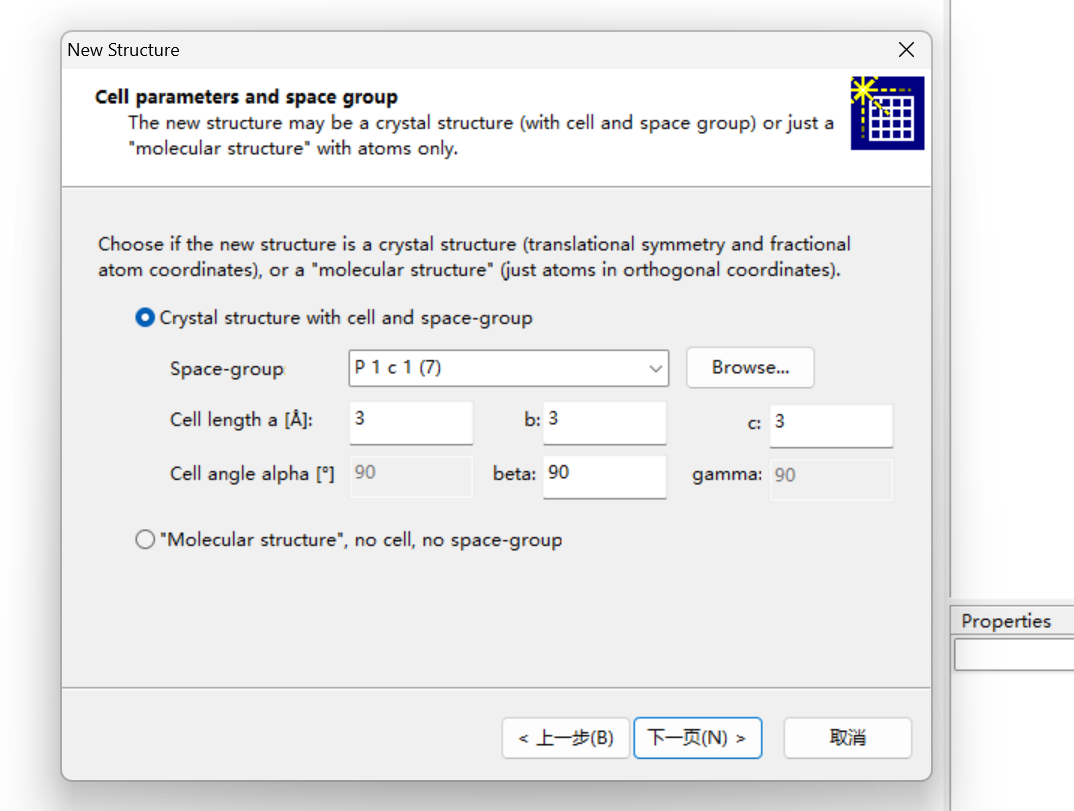
\includegraphics[width=0.44\textwidth]{assets/symmetry/glide/a.png}}
  \hfill
  \subcaptionbox{非对称单元原子（Si）添加}{%
    \includegraphics[width=0.44\textwidth]{assets/symmetry/glide/b.png}}
  \caption{滑移面（$P\,1\,c\,1$）演示的参数设置}
  \label{fig:sym-glide-param}
\end{figure}

\begin{figure}[H]
  \centering
  \subcaptionbox{单胞图：2 个原子由 $c$ 滑移面操作相联系}{%
    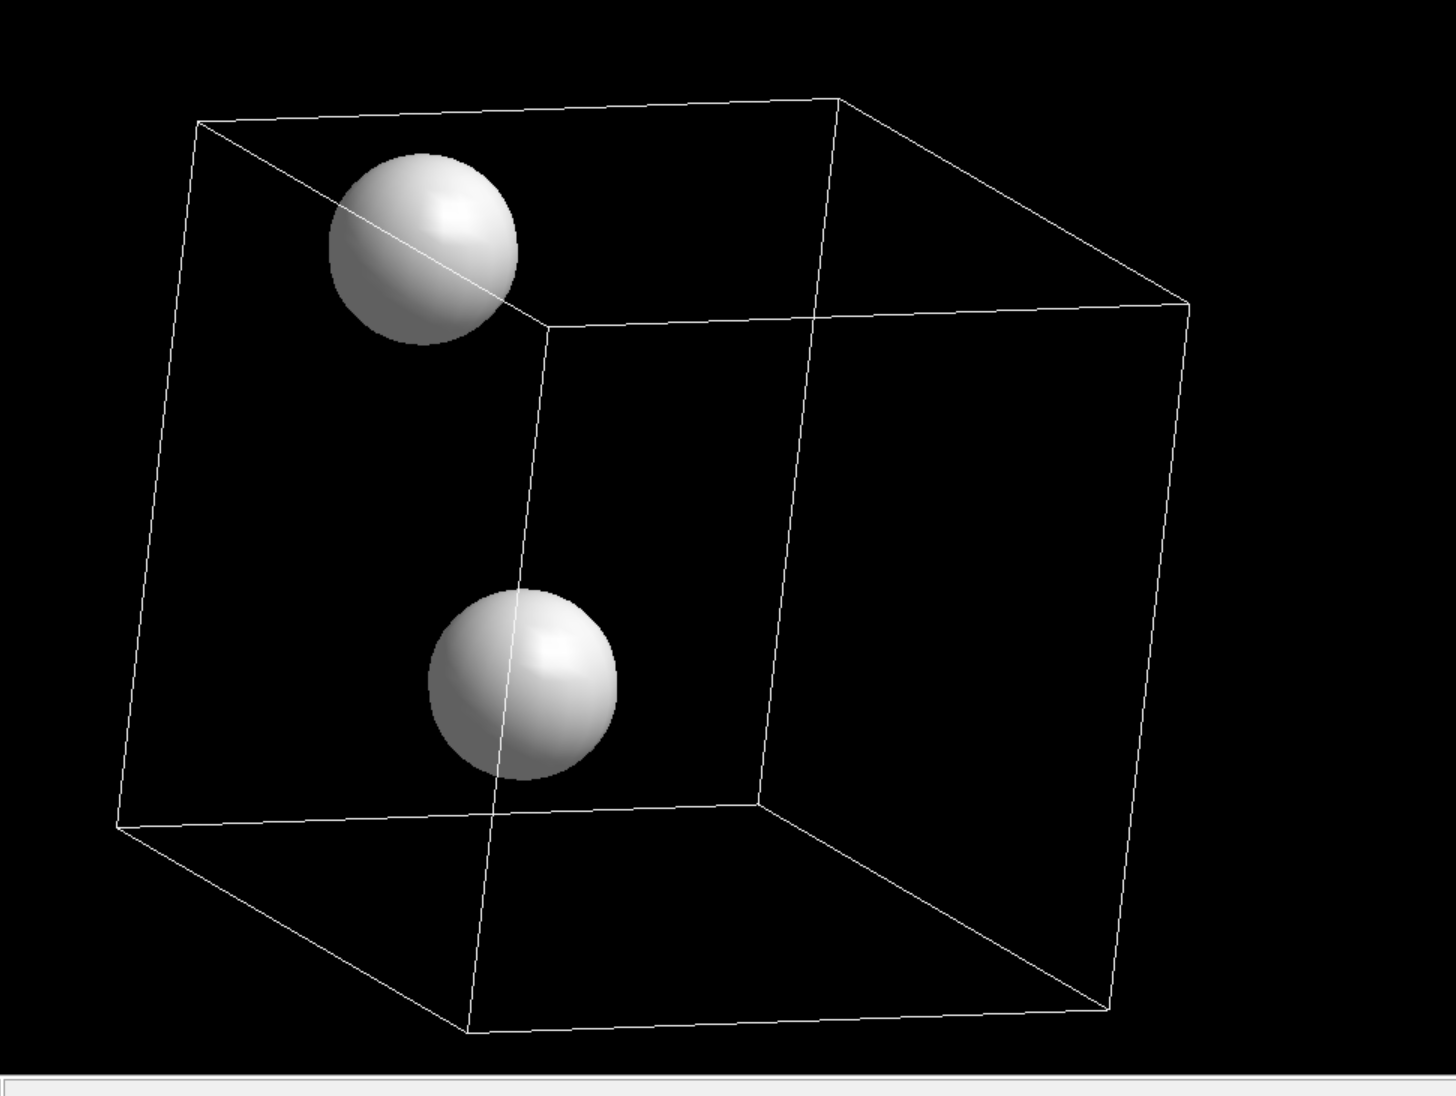
\includegraphics[width=0.44\textwidth]{assets/symmetry/glide/c.png}}
  \hfill
  \subcaptionbox{超晶胞图：相邻原子列沿 $c$ 方向错开半个周期}{%
    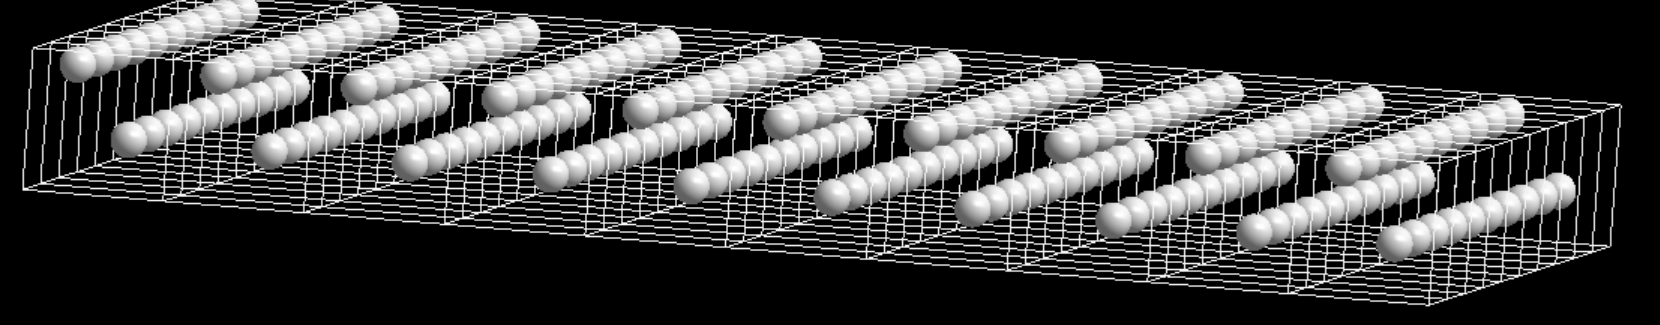
\includegraphics[width=0.44\textwidth]{assets/symmetry/glide/d.png}}
  \caption{滑移面（$P\,1\,c\,1$）的单胞与超晶胞模型}
  \label{fig:sym-glide-model}
\end{figure}

$c$ 滑移面的操作分两步：先经垂直于 $b$ 轴的镜面反映 $(x,y,z)\to(x,\bar y,z)$，再沿
$c$ 方向平移 $1/2$ 个周期，得到
\begin{equation}
  c:\quad (x,y,z)\ \longrightarrow\ (x,\,\bar y,\,z+\tfrac12)
\end{equation}
将 Si 的坐标 $(0.2,0.3,0.4)$ 代入，两个原子的分数坐标为 $(0.2,0.3,0.4)$ 与
$(0.2,0.7,0.9)$（图~\ref{fig:sym-glide-model}(a)）。在单胞中滑移操作只表现为``反映''
（两原子关于镜面等距反向），只有将模型扩展为超晶胞后，才能看到原子沿 $c$ 方向错开
半个周期的``滑移''特征：相邻原子列在 $c$ 方向上相互错位 $c/2$
（图~\ref{fig:sym-glide-model}(b)）——这正是滑移面与纯镜面的区别所在。

\textbf{特征与辨识要点。}滑移面按滑移方向分为：轴滑移面 $a$、$b$、$c$（沿相应晶轴
方向平移 $1/2$）、对角滑移面 $n$（沿面对角线方向平移 $1/2$）与金刚石滑移面 $d$
（平移 $1/4$）。滑移面含平移分量，属微观对称元素。滑移面在衍射上有确定的表现：
$c$ 滑移面垂直于 $b$ 轴时，位于 $(x,y,z)$ 与 $(x,\bar y,z+\tfrac12)$ 的两个原子对
$h0l$ 反射的散射波相位差恒为 $\pi l$，$l$ 为奇数时两者贡献恰好相互抵消——即
\textbf{$h0l$ 中 $l$ 为奇数的反射系统消光}。利用各类对称元素引起的系统消光规律判断
空间群，正是 X 射线衍射结构分析的重要内容。

% ==================== 2.4 小结表 ====================
表~\ref{tab:sym-summary} 汇总了本节六组对称元素演示的空间群、等效位置数与原子分布
特征。

\begin{table}[H]
  \centering
  \small
  \caption{六类对称元素演示的对比}
  \label{tab:sym-summary}
  \begin{tabular}{@{}lllccp{3.6cm}@{}}
    \toprule
    对称元素 & 国际符号 & 演示空间群（No.） & 一般位置数 & 平移分量 & 原子分布与辨识 \\
    \midrule
    反演中心 & $\bar1$ & $P\,\bar1$（2） & 2 & 无 & 关于反演中心等距反向的原子对 \\
    旋转轴 & $3$ & $P\,3$（143） & 3 & 无 & 绕轴 $120^\circ$ 分布，位于垂直轴的同一平面 \\
    旋转反演轴 & $\bar3$ & $P\,\bar3$（147） & 6 & 无 & 上下两层各 3 个，沿轴投影呈``似六重''分布 \\
    镜面 & $m$ & $P\,m\,\bar3$（200） & 24 & 无 & 三组互相垂直镜面，原子镜像成对 \\
    螺旋轴 & $3_1$ & $P\,3_1$（144） & 3 & $c/3$ & 沿轴螺旋上升，不位于同一平面 \\
    滑移面 & $c$ & $P\,1\,c\,1$（7） & 2 & $c/2$ & 反映后沿 $c$ 方向错开半个周期 \\
    \bottomrule
  \end{tabular}
\end{table}

把六组演示放在一起比较，可以看到一条清晰的分界：反演中心、旋转轴、旋转反演轴与
镜面属于宏观对称元素，产生的等效原子由纯旋转、反映或反演相联系，不含平移分量；
$3_1$ 螺旋轴与 $c$ 滑移面则分别带着 $c/3$ 与 $c/2$ 的平移，等效原子沿轴向逐个错开，
这种复合操作特征只有在超晶胞中才显示出来。六种演示基本覆盖了空间群国际符号中的
常见符号类型（旋转轴 $n$、旋转反演轴 $\bar n$、镜面 $m$、螺旋轴 $n_m$ 及各类滑移面
$a$、$b$、$c$、$n$、$d$），回头再看 $P\,\bar1$、$P\,3$、$P\,\bar3$、$P\,m\,\bar3$、
$P\,3_1$、$P\,1\,c\,1$ 这些符号，即可逐字读出它们的含义。对称元素是否含平移分量
（宏观还是微观），决定了单胞内等效原子的空间分布；而对称性同时决定衍射的系统消光
规律，这也是后续物相鉴定与空间群判定的实验基础。

% ==================== 7 结论 ====================
\setcounter{section}{6}
\section{结　论}

本文用 Diamond 完成了 FCC、BCC、HCP、NaCl、金红石、锐钛矿、萤石与金刚石八种结构的
建模，以及六类对称元素的仿真演示。下面按
``结构—方法—对称性''三个方面归纳所得。

八个结构覆盖了金属、离子晶体与共价晶体的主要类型。金属单质中，FCC 与 HCP 的堆积
因子同为 0.7405，区别只在密排层的堆积顺序（ABCABC 与 ABAB）；BCC 的堆积因子降到
0.6802、配位数为 8，却是许多高温相与碱金属的稳定结构。离子晶体的配位数由阴阳离子
半径比决定：NaCl 中 Na$^+$ 取八面体六配位；萤石中 Ca$^{2+}$ 为立方八配位、F$^-$ 为
四面体四配位。TiO$_2$ 的两种晶型同为 TiO$_6$ 八面体配位，差别集中在连接方式：金红石
共棱成链、链间共角，锐钛矿则全部共边。金刚石结构以 $sp^3$ 四面体配位为特征，堆积
因子仅 0.3401，与共价键的方向性密切相关。

方法上，建模的关键是让``空间群—晶格常数—非对称单元原子''三者自洽：参数设对之后，
晶胞填充、晶面显示与配位多面体都只是顺次操作；粉末衍射模拟则把结构模型和真实的
XRD 实验联系了起来。

对称性方面，六类元素的演示把抽象符号变成了可对照的图像：反演中心让原子成对、关于
中心等距反向（$P\,\bar1$ 单胞 2 个原子）；3 次旋转轴给出 3 个共面原子（$P\,3$）；
旋转反演轴 $\bar3$ 相当于 $3+\bar1$ 的联合操作，产生上下两层共 6 个原子，沿轴观察时
呈``似六重''的假象；$P\,m\,\bar3$ 中原子关于三组互相垂直的镜面镜像成对；$3_1$ 螺旋轴
与 $c$ 滑移面含平移分量，螺旋上升与错位排列只有在超晶胞中才显示出来。这些演示说明：
对称性既决定单胞内的原子分布，也决定衍射的系统消光规律。

通过本次建模与演示，笔者对``空间群—原子占位—配位多面体—堆积方式''的分析路径有了
具体体会，也熟悉了用对称符号反推结构信息的做法；这些模型与截图将直接用于后续 XRD 谱
的指标化对照。

% ==================== 致谢 ====================
\section*{致　谢}
\addcontentsline{toc}{section}{致　谢}

感谢 X 射线晶体学课程任课老师的悉心讲授与指导，使笔者掌握了晶体学基础与结构建模的
方法；感谢同学在软件操作与讨论中给予的帮助。


% ==================== 参考文献 ====================
\printbibliography[title=参考文献]

\end{document}
